\documentclass[a4paper,12pt]{book}

\pagestyle{myheadings}
\usepackage{blindtext}

\usepackage{pdfpages}
\usepackage{geometry}
\usepackage{newtxmath,newtxtext}
\usepackage{ragged2e}
\usepackage{indentfirst}
\usepackage{titlesec}
\usepackage[utf8x]{inputenc}
\usepackage[romanian]{babel}
\usepackage{combelow}
\usepackage{newunicodechar}
\usepackage{graphicx}
\usepackage{float}
\usepackage[procnames]{listings}

\usepackage{xcolor}

\definecolor{codegreen}{RGB}{166,226,46}
\definecolor{codegray}{rgb}{0.5,0.5,0.5}
\definecolor{codepurple}{rgb}{0.58,0,0.82}
\definecolor{backcolour}{rgb}{0.95,0.95,0.92}
\definecolor{darkblue}{rgb}{0.0,0.0,0.6}
\definecolor{comments}{RGB}{153,71,31}
\definecolor{returnc}{RGB}{174,129,255}

\usepackage[nottoc]{tocbibind}

\lstdefinestyle{mystyle}{ 
	frame = single,
	commentstyle=\color{comments},
	keywordstyle=\color{darkblue},
	numberstyle=\color{codegray},
	stringstyle=\color{codepurple},
	basicstyle=\ttfamily\footnotesize,
	breakatwhitespace=false,         
	breaklines=true,                 
	captionpos=b,                    
	keepspaces=true,                 
	numbers=left,                    
	numbersep=10pt,                  
	showspaces=false,                
	showstringspaces=false,
	showtabs=false,                  
	tabsize=4,
	procnamekeys={def,class},
	procnamestyle=\color{comments},
	%
	literate={pyauddio}{{\textcolor{green}{pyauddio}}}{8}%
	,
	emph={%  
		downto, for, with, self, None, lambda, True, False %
	},emphstyle={\color{darkblue}}%
}

\lstset{style=mystyle}

\graphicspath{ {../Diagrams/} }
\usepackage[font=small,labelfont=bf]{caption}
\newunicodechar{Ș}{\cb{S}}
\newunicodechar{ș}{\cb{s}}
\newunicodechar{Ț}{\cb{T}}
\newunicodechar{ț}{\cb{t}}
\newunicodechar{ă}{\u{a}}
\raggedbottom
\geometry{
	top 	= 2.5cm,
	bottom 	= 2cm,
	inner 	= 2.75cm,
	outer 	= 2cm,
	bindingoffset=0cm,
	headsep = 0.5cm,
	headheight = 0.5cm,
	footskip = 1cm,
}
\title{Lucrare Licenta}
\author{Steleac Raul-Dacian}

\titleformat{\chapter}
{\normalfont\fontsize{20}{14}\bfseries\sffamily}{\thechapter}{1em}{}
\titleformat{\section}
{\normalfont\fontsize{16}{14}\bfseries\sffamily}{\thesection}{1em}{}
\titleformat{\subsection}
{\normalfont\fontsize{14}{14}\bfseries\sffamily}{\thesubsection}{1em}{}

\titlespacing{\chapter}{0cm}{00pt}{30pt}
\titlespacing{\section}{0cm}{40pt}{20pt}
\titlespacing{\subsection}{0cm}{20pt}{10pt}

%\let\OLDthebibliography\thebibliography
%\renewcommand\thebibliography[1]{
%	\OLDthebibliography{#1}
%	\setlength{\parskip}{0pt}
%	\setlength{\itemsep}{0pt plus 0.3ex}
%}
\newcounter{Figcount}


\usepackage[maxbibnames=1,natbib=true,style=numeric,sorting=none,backend=bibtex]{biblatex}
\DeclareBibliographyCategory{cited}
\AtEveryCitekey{\addtocategory{cited}{\thefield{entrykey}}} 
\newcommand{\size}[2]{{\fontsize{#1}{0}\selectfont#2}}
\newenvironment{sizepar}[2]
{\par\fontsize{#1}{#2}\selectfont}
{\par}
\usepackage{filecontents}

\bibliography{Bibliography}
\nocite{*}

\renewcommand{\lstlistingname}{Algoritm}

\begin{document}
	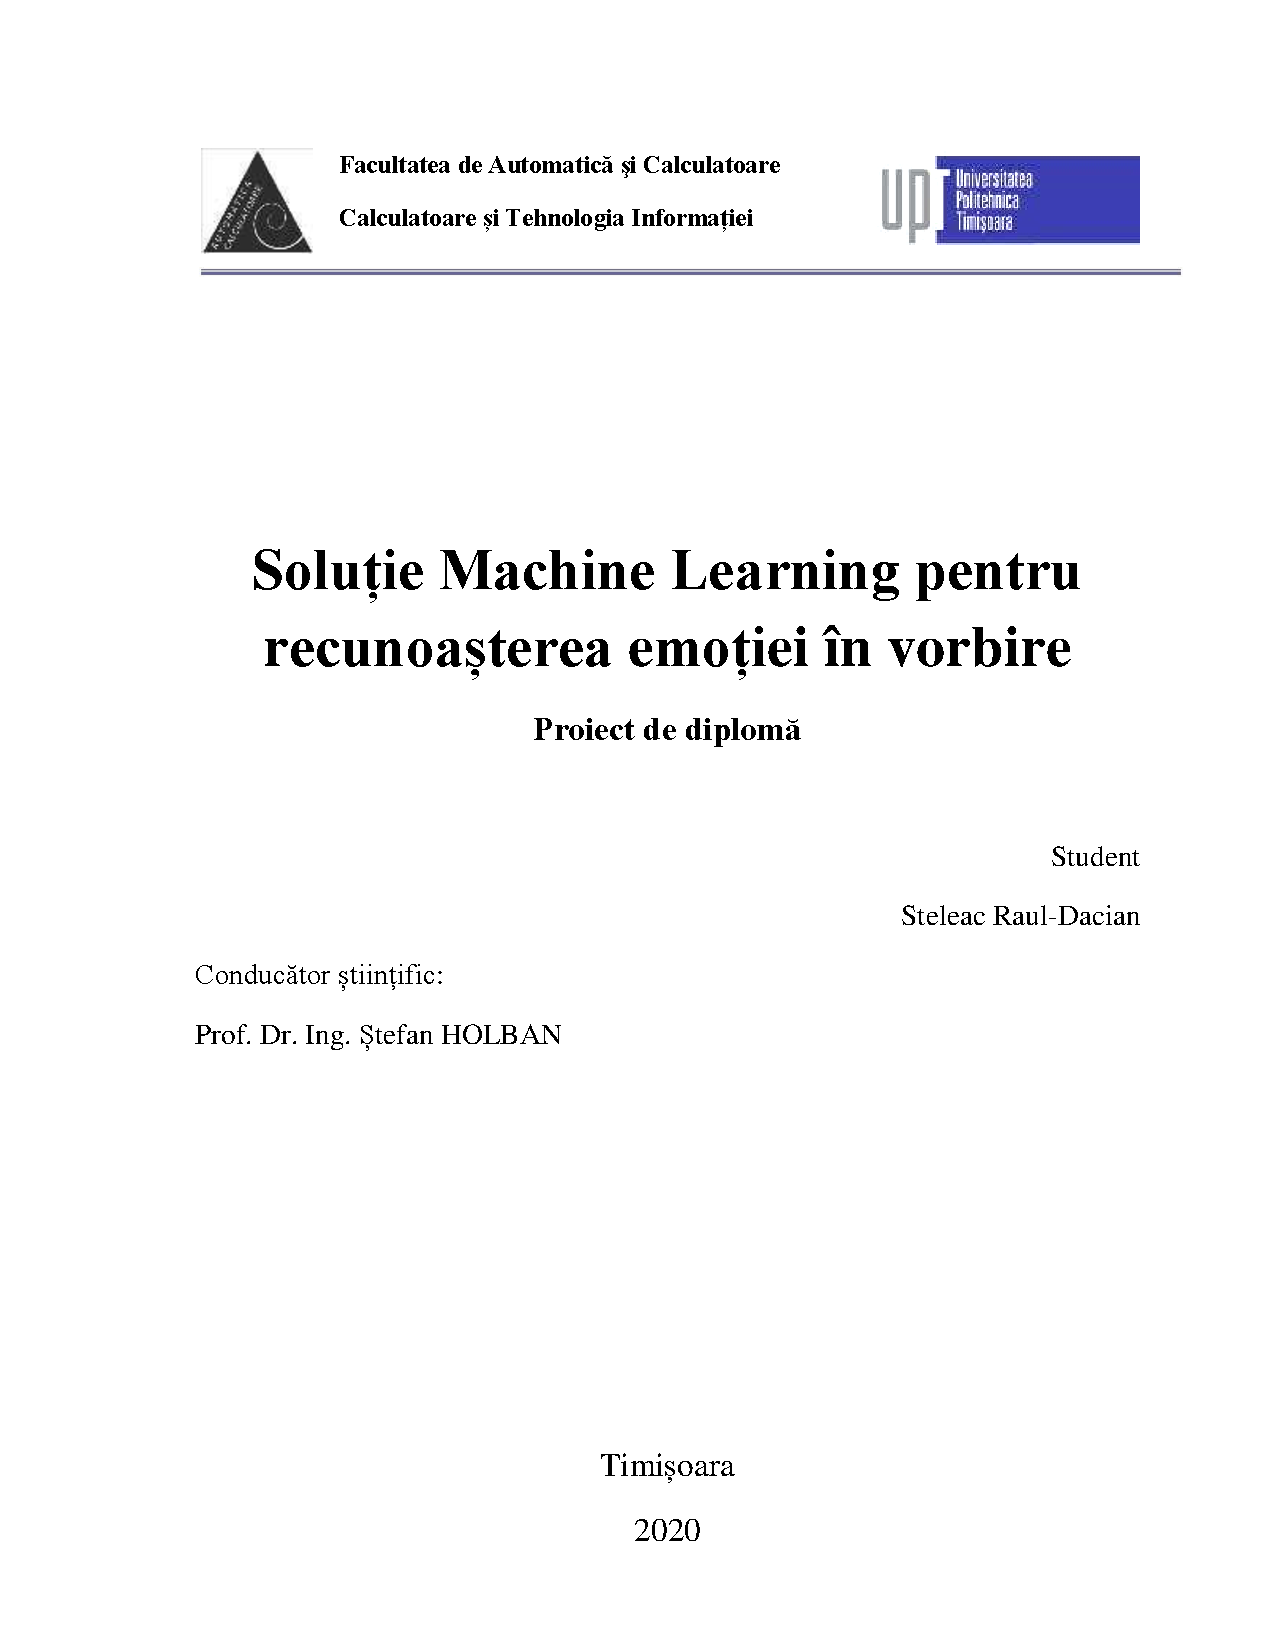
\includepdf{title_page}
	\clearpage
	\thispagestyle{empty}
	\tableofcontents
	\thispagestyle{empty}
	\clearpage
	\newpage 
	\thispagestyle{empty}
	
	\chapter{Introducere}
	
		\section{Prezentarea Problemei}
						
			\setlength{\parindent}{0.8cm}
			
			Comunicarea este o capacitate esențială pentru specia umană, fiind cea mai naturala si principala modalitate de transmitere a informației într-un mod direct. Totuși pe lângă informația lingvistică o mare parte din informațiile prezente în conversațiile pe care le avem zilnic sunt ascunse în emoțiile cu care rostim și articulăm diferite cuvinte, silabe și chiar litere. Urechea umană este capabilă să determine și cele mai mici inflexiuni din vocile participanțiilor la conversație pentru a reuși să capteze cât mai bine sensul acesteia. Astfel, este de așteptat că mașinile care urmează să facă parte de acum din aceste conversații să fie la fel de competente din aceasta privința. Domeniul stintific care se ocupă cu crearea unor modele de tip "Machine Learning" pentru determinarea emoțiilor dintr-un discurs se numește "Speech Emotion Recognition", sau SER. \par
			
			Proiectul de diploma propus de mine incearca sa creeze o solutie pentru recunoasterea emotiei in vorbire si sa ofere un mediu de utilizare propice printr-o interfata grafica care contine diferite functionalitati de configurare a modelului, extragere de statistici si inregistrare. Utilizatorul are astfel optiunea de a antrena solutia SER propusa de mine cu diferite configuratii de parametrii cat si de a testa modelul obtinut pe semnale audio pre-inregistrate sau inregistrate pe loc.\par
			
			\subsection{Importanta Informatiei Emotionale}
				Informatia emotionala este prezenta in orice conversatie si reprezinta un punct de reper catre sensul din spatele cuvintelor vorbitorilor. Emotiile pot pe de o parte sa adanceasca sensul unor anumite cuvinte sau chiar sa il intoarca pe dos daca sunt folosite in ipostaze contradictorii. De exmeplu, propozitiile sumbre ar putea fi considerate glume daca sunt rostite intr-un mod umoristic la un moment potrivit sau propozitiile pozitive pot sa devina sarcastice pe un ton trist. Un participant la conversatie care nu poate sa inteleaga aceste concepte va fi astfel puternic dezavantajat. Deoarece oamenii sunt mai mult sau mai putin experti in determinarea acestor informatii emotionale, dorim ca si viitoarea generatie de vorbitori, agentii AI, sa poata sa realizeze aceasta performanta.\par
				In trecut, majoritatea studiilor legate de rolul emotiei umane in acustica 	unui discurs au fost facute in psihologie. Blanton, 1915 \cite{blanton}, de exemplu, a scris ca "efectul emotiei asupra intonatiilor vocii sunt recunsocute de orice persoana. Chiar si cele mai primitive specii pot recunoaste tonuri care reprezinta dragoste, frica sau enervare. Cainii, caii, si multe alte animale pot intelege si chiar parti din limbajul uman. Iar limbajul tonurilor este cel mai vechi si universal dintre toate modurile de comunicare".\par 
				Plecand de la motivatia ca informatia emotinala este folosita in mecanismul de comunicare chiar si a celor mai primitive specii, putem sa ne intrebam care era modalitatea de comunicare a stramosilor nostrii inainte de aparitia cuvintelor. Capacitatea obtinerii unei forme de limbaj nu era posibila pentru specia \textit{Homo erectus}, stramosii speciei \textit{Homo sapiens}, deoarece dezvoltarea vorbirii a necesitat o conexiune directa a cortexului motor central cu muschii intercostali , conexiune care lipseste din constructia coloanei vertebrale ale acestora. Prima specie din familia \textit{Hominidae} care s-au bucurat de acest beneficiu a fost \textit{Homo sapiens}.  Levinson \& Holler, 2014 \cite{leviholler} sustin conventia ca limbajul a aparut cu aproximativ o suta de mii de ani dupa aparitia speciei umane, \textit{Homo sapiens}, care se estimeaza a fi acum circa trei sute de mii de ani. Astfel printr-un calcul rapid puitem sa determinam ca a existat o perioada de circa o suta de mii de ani in care stramosii nostri, \textit{Homo sapiens}, desi capabili sa folosesaca un limbaj pentru comunicare, nu au facut-o. Christiansen \& Kirby, 2003 \cite{chriskirbi} mentioneaza un consens intre cercetatorii acestui domeniu in legatura cu pasii necesari prin care o specie poate sa dezvolte un limbaj. Mai exact, consensul este ca inainte de aparitia limbajului cateva "pre-adaptari" au trebuit sa apara in descendentii familiei \textit{Hominidae}. Desi cercetatorii nu sunt complet de acord in legatura cu lista acestor "pre-adaptari", un candidat propus de majoritate a fost abilitatea de folosi asa numite "simboluri". In acest context, simbolurile reprezinta capacitatea de a crea legaturi intre sunete si gesturi arbitrare cu anumite emotii, concepte sau perceptii specifice. Aceste gesutri si suntete au alcatuit astfel primele forme de dialog al speciei umane. Putem sa obesrvam astfel cum desi informatia lingvistica nu exista inca in comunicarea speciei umane, informatia emotionala a fost inclusa inca de la primele forme de interactiuni sociale.\par 
				
				
				Cantitatea de informatie din spatele emotiilor pe care le folosim astazi in limbajul modern ramane la fel de importanta ca pe vremea stramosilor nostri. De aceea, in prezent, studiul importantei emotiei dintr-o conversatie este extins si in domeniul calculatoarelor prin inteligenta artificiala. \par	
			\subsection{Prezentare SER}
				Domeniul "Speech Emotion Recognition", sau SER, are ca scop final construirea unui model de tip "Machine Learning" care sa primeasca de la intrare o inregistrare audio, o parte dintr-o conversatie, si sa genereze la iesire o emotie, care sa fie reprezentativa pentru acea inregistrare. \par
				Recunoasterea emotiilor in vorbire este o problema care a starnit curiozitatea adeptilor domeniului inteligentei artificiale de cateva decenii. Daellert et al., 1996 \cite{dellaert} au deschis granitele acestui domeniu in 1996 cu primul articol stintific care incearca sa combata acest subiect. Acestia au incercat sa clasifice patru tipuri de emotii prin folosirea unor date de intrare asa numite "prosodice" ca tonalitatea, intensitatea, frecventa sau amplitudinea folosind trei tipuri de modele de clasificare diferite "Maximum Likelihood Bayes classifier" (MLB), "Kernel Regression"  (KR) si "K-nearest neighbors" (KNN). Aceasta implementare este una reprezentativa pentru combaterea recunoasterii de emotii in vorbire, realizand o separare clara intre cele doua module arhitecturale principale: extragerea datelor si clasifiactorul care urmeaza sa fie antrenat. Discrepanta dintre arhitecturile folosite in prezent si cea prezentata mai sus ramane insa observabila. Chiar daca datele de intrare prosodice sunt inca folosite astazi, cresterea drastica a puterii de procesare a dus la folosirea unor arhitecturi cu retele neuronale adanci care adopta ori mai multe tipuri de date de intrare ori direct semnalul audio neprocesat, daca modelul realizeaza extragerea datelor printr-o maniera automata, "end-to-end models". \par		
				
				Diferentele arhitecturale sunt totusi un semn benefic, fiind reprezentative pentru evolutia domeniului de cercetare. SER si-a pastrat popularitatea in ultimele doua decenii detinand un numar bogat de articole stintifice pe aceasta tema. Aceste articole aduc noi interpretari atat din punctul de vedere al extragerilor caracteristicilor semnalului audio folosite ca date de intrare cat si a modelului folosit pentru antrenare. Totusi, desi noi idei si arhitecturi contiuna sa apara anual, aceasta tehnologie nu a reusit sa atinga inca o acuratete destul de satisfacatoare pentru a fi lansata pe piata. \par
					
				O tehnologie indrudita a recunoasterii emotiei in vorbire, "Speech Recognition" care incearca sa determine informatia lingvistica dintr-o conversatie, a reusit sa revolutioneze interfetele de comunicare dintre om si masina. Aceasta tehnologie isi gaseste locul in majoritatea telefoanelor, calculatoarelor, masinilor si chiar a unor echipamente din jurul casei. Alexa, Cortana si Siri sunt cateva nume pe care majoritatea persoanelor le cunosc fara sa le asocieze cu o fata sau o persoana. Acesti agenti inteligenti obtin rezultate exceptionale in capacitatea lor de a mentine o conversatie cu clientii si de a raspunde la anumite cerinte ale acestora. Cu toate acestea, algoritmii de "Speech Recognition" nu resuesc mereu sa raspunda corect la afirmatiile utilizatorilor deoarece nu iau in considerare si partea emotiva a dialogului. Pentru a obtine o inerfata de comunicare om-masina completa, informatia emotionala este esentiala. Prin diferite intonatii sensul cuvintelor poate fi schimbat complet iar un algoritm care se focuseaza doar pe informatia lingvistica va ramane inflexibil la aceste intonatii generand astfel rezultate eronate. \par
					

		\section{Motivatia Problemei}
			Recunoasterea emotiei in vorbire reprezinta un subiect extrem de interesant atat din punct de vedere aplicativ cat si personal. Potentialul acestui domeniu este ridicat din cauza numarului ridicat de aplicatii care pot beneficia prin incorporarea unui astfel de sistem. Modurile in care un sistem SER poate fi utilizat sunt limitate doar de nivelul tehnologic curent si imaginatia programatorilor.
			\subsection{Motivatie aplicativa}				
					Aplicatiile in care aceasta tehnologie poate fi folosita in viitor sunt greu de estimat, deoarece orice interfata om-masina care foloseste dialogul ca modalitate de transmitere de informatii poate beneficia prin includerea unui astfel de algoritm. Cu toate acestea, o gama larga de aplicatii din prezent sunt deja succeptibile la a fi imbunatatite prin intermediuli introducerii unui model SER. \par
					
					Un bun exemplu este incorporarea unui algoritm SER in mecanismul de \textit{"feed-back"} al unei companii. Principala modalitate prin care firmele din zilele noastre incearca sa capteze parerea publicului asupra unui produs este prin folosirea unor chestionare. Chiar daca aceste chestionare iau loc in scris sau telefonic aduc anumite limitari. In prima situatie apare incertitudinea asupra onestitatii raspunsurilor oamenilor iar in cea de a doua situatie apare limitarea personalului disponibil care sa asculte raspunsurile intervievatiilor in decursul chestionarului. Un sistem alcatuit dintr-un algoritm de "speech emotion recognition" impreuna cu unul generic de "speech recognition" poate capta atat informatia lingvistica cat si cea emotionala din raspunsurile la intrebarile chestionarelor, notand atat cuvintele in sine cat si gradul de credibilitate bazat pe implicarea emotionala a participantului. \par
		
					Un alt exemplu ar fi implicarea modelelor SER in tehnologiile care ne usureaza deja viata de zi cu zi. Agentii inteligenti si diferitele tipuri de roboti,ca de exemplu Huahu et al., 2010 \cite{huahu}, care apar tot mai des in prezent in apropierea oamenilor pot gasi un mare avantaj in determinarea emotiilor clientilor cand incearca sa raspunda cat mai exact la nevoile acestora. De exemplu un astfel de agent inteligent incorporat intr-o masina poate detecta daca in timpul mersului soferul este implicat intr-o cearta sau o discutie cu un puternic impact emotional. Daca acest lucru este adevarat sistemul SER poate sa il indrume pe sofer sa opreasa masina pana cand discutia s-a terminat pentru evitarea unui accident din cauza lipsei de atentie. Alexa sau Siri, care sunt folosite la nivel  global de mii de oameni in jurul casei, pot sa incerce sa ofere raspunsuri care sa linisteasca un client nervos sau sa introduca mici glume pentu a incerca sa inveseleasca un client trist.\par 
						
					Acesti alogritmi ar putea fi folositi si pentru a eficientiza educatia. Prin introducerea unor receptoare de emotii profesorii pot determina starea emotionala a studentiilor si pot extrage informatii pentru imbunatatirea calitatii orelor de curs. De exemplu profesorul poate folosi modelul de recunoastere a emotiilor pentru determinarea continua a interesului studentiilor sau pentru a crea strategii prin care sa ridice moralul clasei cand vine vorba de anumide subiecte predate care ii pot descuraja sau plictisi pe acestia. \par
					
					Alte exemple care merita mentionate sunt folosirea acestor tipuri de algoritmi in: statii de call center (Gupta \& Rajput, 2007 \cite{gupta}), jocuri video ( Szwoch \& Szwoch, 2015 \cite{szwoch}) sau evaluare pshiologica ( Lancker et al., 1989 \cite{lancker} ). \par 								
			\subsection{Motivatie Personala}				
					Tema recunoasterii de emotii a inceput sa ma intrige cand mi-am pus problema construirii unui psiholog artificial. Desi crearea unui astfel de terapist artificail este putin probabila, recunoasterea de emotii ramane o problema cu potentialul de a fi rezolvata. In subiecte ca recunoasterea obiectelor, fetelor, si chiar a cuvintelor rostite s-a obtinut o acuratete destul de satisfacatoare pentru a fi introduse pe piata. Pentru domeniul recunoasterii de emotii in vorbire insa, acest lucru nu este valabil inca. \par
					
					Diferite carti, filme sau seriale din zilele noastre prezinta o multitudine de posibile utopii tehnologice care ar putea sa devina realitate in urmatoarele decenii sau secole. Desi acestea sunt doar scenarii Sci-Fi, una din ideile comune este existenta unei interfete de comunicare verbala de la om la masina aproape perfect identica, din punct de vedere calitativ, cu cea de la om la om. Sistemele de "Speech Recognition" deja existente ofera un bun exemplu prin succesul lor care sustine importanta unei astfel de tehnologii, dar si a popularitatea ei in randul publicului. SER incearca sa imbunatateasca aceste conversatii oferind capacitatea masinilor de a intelege si emotiile din spatele cuvintelor. Acest trasnfer de informatie emotionala mi se pare extrem de interesant deoarece poate sa ne ofere pe viitor capacitatea de a ne intelege mai bine propriile emotii dar si de a crea agenti inteligenti care sa se aproprie cat mai puternic de o inteligenta de o generalitate asemanatoare cu a noastra. \par
					
					Lipsa acestui domeniu de pe piata cat si potentialul pe care il detine m-a motivat sa aleg acest subiect pentru proiectul de diploma. Desi implementarea pe care o propun obine rezultatea asemanatoare cu unele din cele mai de success soluti gasite in diferite articole stintifice, nu reuseste sa obinta inca o acuratete si o  generalitate destul de ridicata pentru a permite comercializarea acestor alogritmi. Solutia propusa de mine reprezinta o alta incercare de a aduce acest domeniu mai aproape de acel nivel necesar care il va face valabil publicului. \par 
										
			\section{Obstacole in studiul SER}	\label{obstacole}	
				Cu toate ca potentialul sistemelor de recunoastere de emotii in vorbire este ridicat, aceasta tehnologie nu a reusit sa obtina acuratetea necesara pentru a face parte din sistemele artificale de comunicare verbala din prezent. Principalele piedici care despart domeniul SER de majoritatea aplicatiilor de "Machine Learning" si ii incetinesc acestuia progesul sunt legate de dificultatea obtinerii unui set de date de intrare satisfacator comparativ cu complexitatea problemei si lipsa unor caracteristici de intrare care sa fie reprezentative pentru detectarea emotiei. Aceste doua considerente au alcatuit in decusul ulitmelor doua deceni obstacole serioase in studiul si dezvoltarea modelelor de recunoastere de emotii deoarece implica necesitatea folosirii unor resurse costisitoare din punct de vedere financiar, temporal si uman.\par
				
				\subsection{Impactul bazelor de date}
					Bazele de date aferente recunoasterii de emotii in vorbire sufera atat din punct de vedere cantitativ cat si calitativ. Bjorn, 2018 \cite{bjorn1} sustine ca o particularitate a acestui domeniu de cercetare este subiectivitatea si incertitudinea ridicata in construirea bazelor de date. \par 
					Exista doua tipuri principale de baze de date in domeniul SER in functie de modul in care acestea sunt obtinute: jucate (de actori) sau spontane, iar ambele modalitati sufera de diferite dezavantaje. \par
					Pe de o parte, majoritatea bazelor de date care exista sunt alcatuite prin inregistrarea unor actori profesionisti, studenti la actorie sau chiar persoane care primiesc o anumita propozitie si incearca sa o rosteasca in cadrul unei anumite emotii. Din punct de vedere calitativ, devine destul de aparent cum aceste emotii pot fi exagerate, lucru care face ca clasificatorul obtinut sa fie superficial in cazul detectarii emotiiolor reale. Pe langa aceasta problema, obtinerea bazelor de date implica si o perioada de verificare si filtrare. Inregistrarile obtinute sunt cedate unor persoane, care nu au participat in partea de inregistrare, pentru a le clasifica. Daca in urma acestui proces rezultatul este emotia intentionata initial atunci inregistrarea este declarata valida si va fi folosita pentru antrenare. Totusi, problema principala este ca nici oamenii nu reusesc sa determine perfect emotia predominanta dintr-un discurs. Acest lucru afecteaza direct corectitudinea bazei de date si acuratetea modelului. Din punct de vedere cantitativ, in procesul de antrenare sunt astfel implicate destul de multe persoane. Acest lucru ingreuneaza obtinerea unor seturi de date numeros deoarece acest proces devine dificil din punct de vedere financiar cat si temporal.\par
					Pe de alta parte, exista seturi de date in care emotiile nu sunt jucate de actori profesionisti , ci sunt extrase din inregistrari in care acestea apar in mod spontan. In alcatuirea acestora, se aleg parti din diferite talk show-uri, inregistrarii din call center-e, discutii la radio, si alte surse similare, iar apoi se depisteaza si se extrag fragmentele bogate in emotie. Un exemplu de acest tip de baza de date este "Multimodal EmotionLines Dataset" (MELD) \cite{meld}, in care s-au preluat parti din episoadele celebrului serial "Friends". Pe langa ca obtinerea datelor devine mai dificila atat din punct de vedere legal cat si etic, apare aceasi problema ca in varianta precedenta in care emotia depistata depinde doar de perceptia persoanei care clasifica inregistrarea, astfel posibilitatea aparitiei de erori nu este evitata. \par
					Concluzia pe care o putem trage este ca indiferent de varianta aleasa nu putem scapa de incertitudinea adusa de discernamantul uman in clasificarea datelor de intrare. Multe modele propuse sustin ideea folosiri inregistrarilor atat din prima ca si din a doua categoria pentru a echilibra dezavantajele impuse de ambele. \par
					Un alt obstacol intampinat de mine a fost ca deoarece realizarea acestor date este asa de dificila, multe baze de date sunt private si necesita sume mari de bani pentru obtinerea lor. Din acest motiv am fost limitat din privinta datelor de intrare pe care le-am putut folosi.
				
				\subsection{Dificultatea extragerii informatiei emotionale} \label{dif_fex}
					O alta mare dilema cu care s-au confruntat multe articole stintifice a fost determinarea unui set de caracteristici ale semnalului audio care sa eficientizeze clasificarea emotiei. Din punctul de vedere al extragerii informatiei emotionale momentan exista doua modalitati principale: folosirea unor caracteristici obtinute matematic prin formule predefinite (hand-crafted feaures) sau prin folosirea unor retele neuronale care prin antrenare sa gaseasca automat cele mai eficente informatii din datele de intrare (end-to-end features). \par
					In cazul in care se folosesc coeficienti obtinuti prin formule matematice generice ca "Mel-frequency cepstrum coefficiants", "Roll-off coeficiants", "detas and delta deltas" etc., nu s-a gasit un set de caracteristici de acest tip care sa fie considerate ideale pentru obtinerea informatiei emotionale. Coeficientii insirati mai sus sunt preluati din "Speech Recognition" pentru ca reprezinta caracteristicile necesare identificarii informatiei lingvistice. Totusi, nu s-a demonstrat care dintre acestia pot fi la fel de benefici si in cazul determinarii emotiilor, lucru care face ca majoritatea studiilor in SER sa foloseasca seturi caracteristici de intrare diferite. \par
					In cazul in care se folosesc coeficienti obitinuiti prin retele neuronale, desi se crede ca acestia sunt mai subiectivi sarcinii de detectare a emotiei, deoarece fac parte din procesul de antrenare al clasificatorului, nu putem sa facem o inferenta directa pe ei. Deoarece nu putem intelege sau replica calculele realizate in diferitele retele neuronale folosite nu putem determina ce semnifica rezultatul fiecarui nivel din retea, cu atat mai putin a fiecarui nod. \par
					Ambele variante au reusit sa produca rezultate performante, iar multe studii s-au realizat in gasire solutiei celei mai eficiente in ambele situatii. Cu toate a acestea cele doua nu reusesc sa rezolve problema initiala, adica gasirea unui set de caracteristici reprezentative pentru emotia din inregistrarile audio. \par
					\hfill \par
					Studiul recunoasterii emotiei umane este un domeniu de cercetare in continua crestere si are ca scop final obtinerea unui model capabil sa determine, inteleaga si raspunda la diferitele emotii prezentate de utilizatorul uman. Desi natura problemei implica diferite dificultati cand vine vorba de gestionarea bazelor de date si extragerea informatiilor relevante din semnalul audio, aceste probleme pot fi rezolvate prin aplicarea diferitelor tehnici prezente in lumea inteligentei artificiale de astazi. In acest mod, detectarea emotiilor din vorbire ramene un domeniu de studiu viabil care are potentialul sa aduca imbunatatiri puternice in interfetele de comunicare om-masina din viitorul apropiat. \par
					Structura capitolelor care urmeaza sa detalieze solutia propusa in aceasta lucrare de diploma atat pentru sitemul de recunoastere a emotiilor in vorbire cat si pentru interfata grafica este urmatoarea:
					\begin{itemize}
						\item Capitolul 2 - Analiza stadiului actual in domeniul problemei, descrie componentele necesare pentru alcatuirea unui sistem SER, trei exemple de arhitecturi de succes din domeniu si o scurta prezentare a solutiei propuse.
						\item Capitolul 3 - Bazele teoretice, prezinta conceptele teoretice care stau la baza arhitecturii sistemului SER, incluzand metodele folosite pentru extragerea caracteristicilor de intrare si componentele modelului clasificator. 
						\item Capitolul 4 - Descrierea implementarii, detaliaza tehnologiile folosite, descrierea secventelor de cod care constituie componentele principale ale lucrarii si utilizarea interfetei grafice.
						\item Capitolul 5 - Rezultate si experimente, enumerarea si descrierea diferitelor configuratii experimentale incercate si a rezultatelor obtinute comparativ cu alte solutii din domeniu.
						\item Capitolul 6 - Concluzii, prezinta un sumar al lucrarii de diploma impreuna cu o lista de posibile ibunatatiri viitoare ale solutiei de recunoastere a emotiilor in vorbire propuse.
					\end{itemize} 
					
	\chapter{Analiza stadiului actual în domeniul problemei} \label{introdP}
				Definim un sitem SER ca o colectie de metodologii care proceseaza semnalele audio aferente unui discurs pentru a detecta emotia incorporata in ele. Ca orice alta problema de clasificare, un sistem SER trebuie sa indeplineasca un anumit set de pasi, care odata organizati cronologic constituie modelul "Machine Learning" propus. \par
				
				Orice sistem SER necesita un clasificator, o entitate care constituie medota de invatare supervizata. Un astfel de sistem supervizat implica folosirea unor date catalogate. In cadrul recunoaterii de emotii in vorbire datele de intrare sunt semnalele audio cu emotiile incorporate. Aceasta forma nu este una eficienta insa pentru detectia acelor emotii, astfel, prin aplicarea diferitelor tehnici, informatia emotinala este extrasa si oferita in noua forma clasificatorului. Inainte ca aceste caracteristici emotinale sa poata sa fi extrase, semnalele trebuie sa treaca si printr-un stagiu de preprocesare.\par
				
				In continuare voi prezenta pasi necesari in ordinea lor cronologica si voi mentiona cateva din configuratiile alese de dezvoltatori pentru rezolvarea recunoasterii de emotii in vorbire.
				\section{Tipologii arhitecturale in SER} 
					\subsection{Preprocesarea datelor de intrare}
						Preprocesarea datelor este primul pas in construirea majoritatii modelelor "Mahine Learning". In "Speech Emotion Recognition", preprocesarea datelor este vitala deoarece poate elimina multe din dezavantajele existente in bazele de date din aceasta ramura a inteligentei artificiale.\par
						Semnalul brut trece in prima faza printr-un proces de partitionare in segmente de lungime fixa. Acesta partitionare este avantajosa pentru algoritmii SER deoarece permite determinarea relatiilor temporale din interiorul inregistrarii (fiecare segment, "frame", fiind considerat un punct pe axa temporala). Urmatorul pas in procesul de preprocesare este aplicarea unor functii fereastra pe fiecare segment. Utilizarea functiilor fereastra are ca scop reducerea pierderii de informatii dupa aplicarea transformarilor Fourier care apare din cauza discontinuitatii de la marginea segmentelor. \par
						Cei doi pasi prezentati anteriori sunt necesari pentru a aduce semnalul audio intro forma care face antrenarea posibila. Din acest motiv, acestia sunt prezenti in orice model care foloseste semnalul sonor ca date de intrare. \par
						In continuarea fazei de preprocsare diferite implementari a modelelor SER opteaza sa folsoeasca diferite tehnici care aduc avantaje serioase in faza de antrenare. Cateva din principalele tehnici folosite sunt:
						\begin{itemize}
							\setlength\itemsep{0pt}
							\setlength{\itemindent}{1.5cm}
							\item Normalizare per vorbitor
							\item Normalizare in functie de sex
							\item Normalizare per baze de date
							\item Algoritmi de reducere a zgomotelor
							\item Algoritmi pentru identificarea segmentelor ce contin o voce umana
							\item Reducerea dimensionalitatii
						\end{itemize}
						Alegerea acestor tehnici este complet subiectiva fiecarei implementari, iar avantajele aduse sunt cantarite in comformitate cu tipul de clasificator folosit. De exemplu, normalizarea per vorbitor reduce impactul diferentelor legate de tonalitatea vocii sau a microfonolui folosit de fiecare vorbitor. Acest tip de normalizare a inregisrat deja un succes intr-un sistem SER detaliat in Bjorn et al., 2010 \cite{spnorm}.
					\subsection{Extragerea Datelor}
						Extragerea caracteristicolor semnalului audio reprezinta un aspect de mare importanta in domeniul recunoasterii emotiilor in vorbire. Obtinerea unui set de caracteristici care sa curpinda informata emotionala cat mai precis are un impact consioderabil asupra acuratetii modelului clasificator. Diferite configuratii de aceste seturi de date au fost propuse pentru sistemele SER, dar, cum am mentionat si in sub-capitolul \ref{dif_fex}, nu s-a ajuns la un consens care sa faciliteze recunoasterea emotiilor. \par
						In total exista patru tipuri de caracteristici care pot fi extrase din semnalul audio, dar majoritatea articolelor stintifice din SER se concentreaza pe cele prosodice si spectrale.\par
						Oamenii se folosesc de durata, intonatie si intensitate pentru a crea diferitele secvente sonore atunci cand rostesc un discurs. Incorporarea acestor prosodii induce caracterul natural in convorbirile noastre. Koolagudi et al., 2012 \cite{koolagudi} sustin ca in literatura stintifica, caracteristicile prosodice ca energia, duratia, amplitudinea si derivatele acestora sunt considerate a fi puternic corelate cu emotiile \cite{dellaert,hcf2,hcf3}. Caracteristici ca minimul, maximul, media, variatia, lunigimea si deviata standard a energiei semnalului audio, si functii similare ale amplitudinii sunt folosite astfel ca surse de informatii prosodice in majoritatea sistemelor SER. \par
						Cand un sunet este produs de un om, acesta trece prin tractul vocal si este puternic influentat de forma acestuia. Caracteristicile acestui tract vocal sunt foarte bine ilustrate in domeniul frecventa. Pentru a profita de aceste informatii se folosesc caracteristicile specializate pe extragerea informatiei din domeniul frecventa, denumite spectrale. Acest tip de caracteristici sunt obtinute prin folosirea celebrelor transformate Fourier. Exemple ale unoara din aceste tipuri de caracteristici folosite in recunoasterea emotiei in vorbire sunt: Mel Frequency Cepstral Coefficients (MFCC), Linear Prediction Cepstrum Coefficients (LPCC), Gammatone Frequency Cepstral Coefficients (GFCC) etc. \par 
						Tehnica care de extragere de informatii care foloseste formule matematice pentru determinarea caracteristicilor prezentate mai sus se numeste in domeniul stintific "hand-crafting". Desi aceasta tehinca a obtinut rezultate destul de satisfacatoare in ultiemele decenii din cazua dezavantajelor prezentate in sub-caiptolul \ref{dif_fex} multe implementari mai noi ale sistemelor SER incearca sa realizeze extragerea caracteristicilor de intrare intr-o maniera automata. \par
						"End-to-end modeles" se refera la o tehnica de automatizare completa a modelelor "Machine Learning" prin care inclusiv extragerea datelor este obtinuta prin antrenare. In SER acest lucru se realizeaza de obicei prin extragerea spectogramei Mel din sunetul brut si aplicarea unei retele neuronale convolutionale cu un numar arbitrar de nivele \cite{graves,tzir}. Aceste nivele interpreteaza spectograma ca o imagine generica si isi adapteaza filtrele pentru a extrage caracteristicile considerate importante din aceasta. Prin folosirea acestui tip de extragere de caracteristici, modelul SER poate identifica singur in timpul antrenari ce informatii din semnalul audio sunt cu adevarat importante in cazul recunoasterii emotiilor. Adoptarea acestei tehnici a fost benefica inca cazul multor solutii din SER \cite{graves, tzir, zhang, yuan, adieu, e2e}, si este folosita si in implementarea propusa de mine.
					\subsection{Clasificatorul}
						Un alogritm de clasificare necesita un set date de intrare X, un set de clase de iesire Y, si o functie care realizeaza maparea lui X la Y in forma urmatoare \(f(X)=Y\). Scopul clasificatorului este de a crea o aproximare a functiei \(f\) bazata perechile de antrenare $(x_i,y_i)$ care sa faciliteze predictia corectab in cazul unor noi date de intrare. \par
						
						Procesul de alegerae a unui model de clasificare in domeniul recunoasterii de emotii in vorbire, la fel ca in cazul majoritatii problemelor "Machine Learning" complexe, nu prezinta o solutie general valabila. Studiile pe aceasta tema aleg un astfel de alogritm printr-o maniera empirica. Cu toate acestea, natura problemei face ca un anumit set de algoritmi de clasificare sa fie mai avantajosi.\par 
						Cele mai folositi algoritmi de clasificare in domeniu SER sunt: Hidden Marko Model (HMM), Gaussian Mixture Model (GMM), Support Vector Machines (SVM) si diferite tipuri de retelele neuronale artificiale ca retele convolutionale si recurente. Pe langa acestea au mai fost folosite si alte tehnici ca: Arbori decizionali (DT), k-Nearest Neighbor (k-NN). k-means si Naive Bayes. Pentru a obtine o acuratete cat mai ridicat s-a optat si spre utilizarea unor modele alcatuite prin combinarea mai multor algoritmi de clasificare, Mehmet et al., 2020 \cite{mehmet}.
						
					\subsection{Tehnici de imbunatatire a clasficarii} \label{tehnici}
						Desi multe rezultate bune au fost obtinute in SER prin folosirea doar a pasilor enumerati mai sus, in multe studii s-au demonstrat o imbunatatire a acestor rezultate prin folosirea anumitor tehnici specifice din domeniul "Machine Learning". \par
						Una din aceste tehnici este folosirea unui \textit{mecanism de atentie}. Mecanismul de atenti are ca scop sa focalizeze atentia modelului pe segmentele bogate in informatii. In cazul SER, mecanismul de atentie este folosit pentru a determina segmentele din semnalul sonor care contin un grad de informatie emotionala ridicata si a mari influenta acestora in decizia clasificatorului. Acest mecanism este alcatuit dintr-un numar de ponderi antrenate in procesul de invatare, care se aplica direct pe iesirile retelelor neuronale avand efectul prezentat anterior.  Rezultatele benefice obtinute in urma aplicarii au fost observate in studiile: Misramadi et al., 2017 \cite{misramadi}, Zhang et al., 2019 \cite{zhang} . \par
						
						\begin{figure}[h]
							\centering
							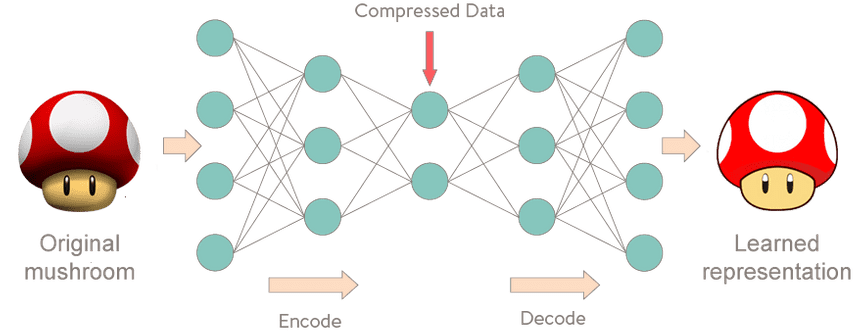
\includegraphics[scale=0.4]{mushroom_encoder}
							\caption{Exemplu de arhitectura auto-encoder. In partea stanga se poate observa imaginea initiala iar in partea dreapta varianta compresata a acesteia obtinuta prin aplicarea auto-encoder-ului.}
							\label{fig:ae}							
						\end{figure}
						O alta tehnica este folosirea unor tipuri de retele neuronale specifice, folosite pentru procesarea datelor de intrare sau chiar crearea unora noi. Aceste retele neuronale sunt numite \textit{autoencoders}. Autoenecoder-ele sunt alcatuite din minim trei nivele. Diferenta fata de retele neuronale apare in faptul ca dimensiunea intrarilor si iesirilor este egala, in timp ce nivelele "ascunse", din interiorul retelei, au dimensiuni mai mici. Astfel autoencoder-ele sunt altacuite din doua parti: "encoder" si "decoder". Encoder-ul compreseaza datele cu scopul de a obtine o varianta cat mai eficienta in care informatiile principale sunt inca pastrate. In schimb, decoder-ul are ca scop aducerea acestei forme compresate la o forma cat mai apropriata de cea initiala. Datele care trec prin aceasta retea sunt filtrate pentru a pastra doar informatia complet necesara, Fig.\ref{fig:ae}. Prin modificari usoare in arthitectura se pot obtine functionalitati complet noi, ca de exemplu "Denoising Autoencoders" (DAE), care dupa aplicarea unui zgomot la datele de intrare au ca scop sa determine ponderile necesare pentru extragerea acelui zgomot si readucerea intrarilor la o forma cat mai apropiata de cea "curata". In SER mai multe tipuri de autoencoder-e au fost folosite in incercarea de a mari acuratetea sistemului: Denoising Autoencoders (DAE) Chao et al., 2014 \cite{dae}, Adaptive Denoising Autoencoders (ADAE) Deng et al., 2014 \cite{adae}, sparse autoencoder (SAE) Deng et al., 2013 \cite{sdae}, adversarial autoencoder (AAE).
						Alte tehnici folosite sunt: 
						\begin{itemize}
							\setlength\topsep{0pt}
							\setlength\itemsep{0pt}
							\setlength{\itemindent}{1cm}
							\item  "Multitask Learning", unde din cauza similitudinii dintre anumie sarcini parti dintr-un clasificator poat fi antrenate pe mai multe probleme marind astfel generalitatea modelului.
							\item "Transfer Learning", Prin aceasta tehnica s-a incercat depasirea dezavantajului legat de lipsa bazelor de date suficiente. Astel diferite implementari se folsoesc de parti din alte modele care au fost pre-antrenate pe probleme similare ca "Speech Recognition" inainte de a incepe antrenarea modelului pe cele specifice SER.
							\item "Voice Detection", Acest algoritm este folsoit pentru exluderea segmentelor care nu contin vocea umana, pentru a reduce posibilele erori aduse de zonele lipsite de informatie emotionala. 						
					\end{itemize}
				
				
				\section{Prezentarea unor implementari din SER} \label{papers}
					Cum am mentionat si in capitolul precedent, "Speech Emotion Recognition" nu a ajuns in punctul in care poate fi pus pe piata. Astfel am decis sa fac o comparatie teoritica incercad sa prezint alte moduri de implementare prezente in cateva articole de cercetare. In continuare voi prezenta trei arhitecturi de sisteme din recunoasterea emotiei in vorbire, care sustin cateva din principalele idei pe care si eu mi-am bazat modelul. Desi prezinta unele similaritati, acestea nu pot fi comparate in mod perfect deoarece folosesc atat baze de date diferite cat si caracteristici de intrare diferite. Deoarece nu exista un mod consacrat de a construi un model SER, avantajele si dezavantajele dintre diferitele implementari devin dificil de identificat. \par		
					
					\subsection{A Cross-corpus Study on Speech Emotion Recognition} \label{prez_multi_domain}
					
					
					Milner et al.(2019) in articolul de cercetare "A Cross-corpus Study on Speech Emotion Recognition" \cite{multi-domain} folosesc un model antrenat pe mai multe baze de date constituite din inregistrari in aceiasi limba, Engleza, cu voci de aceeasi varsta, adulti. Acest articol incearca sa determine beneficiile folosirii  unor emotii jucate de actori profesionisti in combinatie cu unele naturale. Cu atat mai mult, studiul is propune sa prezinte si avantajele folosirii conceptului de "multi-task learning" unde parti din acelasi model sunt antrenate pe diferite sarcini asemanatoare pentru a marii eficienta antrenarii pe acelasi set de date de intrare. \par
					
					Arhitectura implementarii propuse in Milner et al., 2019 \cite{multi-domain} implica folosirea unui set de caracteristici de intrare "hand-crafted" generate prin extragerea coeficientilor MFCC, PLP ("perceptual linear prediction") si COVAREP \cite{covarep} din inregistrarile audio. Modulul clasificator al arhitecturii este extrem de asemanator cu cel folosit de mine in acest proiect fiind constituit din doua nivele de celule recurente LSTM bidirectionale  urmate de un mecanism de atentie, detaliate in \ref{RNN} respectiv \ref{attention}. Setul de emotii clasificate este alcatuit din: fericire, tristete, enervare, surprindere, dezgust, frica si neutru. \par
					
					"Cross-corpus" se refera la antrenarea modelului folosind pe rand cate una din bazele de date dintr-un set si apoi testarea pe fiecare din cele ramase. "Multi-domain" inseamna antrenare pe toate bazele de date si apoi testare pe anumie parti din fiecare. Motivele principale pentru care aceaste tehnici sunt folosite in practica sunt marirea generalitatii modelului si combatrea numarului scazut de inregistrari per baza de date. \par
					
					In acest articol s-au obtinut rezultate foarte bune pentru ambele metode de utilizarea a bazelor de date, acuratete ne-ponderata de  81.94\% in cazul "cross-corpus" si 82\% in cazul multi-domain. \par					
					
					Antrenarea "Multi-domain" nu a fost totusi cea mai de succes metoda folosita in acest articol de cercetarea. Milner et al., 2019 \cite{multi-domain} propun si folisrea tehnicii numite "domain adversarial training", unde pe langa sarcina clasificarii emotiei, o parte din model a fost antrenata sa recunoasca si baza de date din care o inregistrarea face parte. Acest mecanism functioneaza ca un regularizator in procesul de calcularea a erorii, fiind adunat la eroarea rezultata din sarcina principala, SER. Prin introducerea acestei imbunatatiri acuratetea modelului creste atingand, 82.26\%. \par
						
					\subsection{Improved End-to-End Speech Emotion Recognition Using Self Attention	Mechanism and Multitask Learning} \label{end-to-end2}
					
					Li, Yuanchao et al., 2019 \cite{yuan} au reusit sa obtina o acuratetea neponderata cu 14.3\% mai mare fata de solutiile tradionale prin metoda propusa. Aceata metoda se bazeaza pe conceptul de modele "end-to-end". Totusi arhitectura propusa se foloseste si de alte tehnici ca mecanismul de atentie si antrenare "multi-task" pentru a depasi unele obstacole in recunoasterea emotiilor in vorbire. \par
					
					Tehnica de extragere a caracteristicilor de intrare printr-un algoritm "machine learning" face ca toate modulele de procesare din interiorul modelului sa fie antrenabile. De aici apare si numele tehnicii, "end-to-end". Aceste modele sunt extrem de avantajoase in SER, obtinand rezultate incurajatoare \cite{adieu,e2e}. Folosirea unei astfel de extragere "automata" a caracteristicilor semnalelor reduce influenta umana implicata in crearea modelului, deoarece nu mai necesita parearea unor specialisti in domeniul audio pentru a determina cele mai eficente caracteristici de intrare. Avantajele folosirii tehnicii "end-to-end" find descrise mai in detaliu atat in \ref{dif_fex} cat si in \ref{end-to-end}. \par
					
					Asemanator cu solutia propusa in Milner et al., 2019 \cite{multi-domain}, arhitectura foloseste doua nivele recurente bidirectionale la care s-a atasat un nivel de atentie si tehnica de  invatare "multi-task". Cu toate astea, cea de a doua sarcina pe care o executa clasificatorul nu mai este recunoasterea bazei de date ci a sexului persoanei care vorbeste in inregistrare. Prin folosirea acestui timp de antrenare clasificatorul are posibiltatea sa invete diferentele intre caracteristicile vocii unui vorbitor masculin si feminin. \par
					
					Modelul prezentat in acest articol stintific foloseste o singura baza de date de intrare. Astfel modelul devine specializat in a recunoaste emotii pe acel set de date, dar va da un randament mai slab in inferenta pe inregistrari din afara acestui set. Multimea de emotii clasificate este mai redus decat in cazul precedent, fiind constituit din emotiile fericire, tristete, enervare, si neutru , obtinand o acuratete de 82.8\%, care depasete precizia de 68.5\% inregistrata folosind metodele precedente pe aceasi baza de date.
					\subsection{Automatic speech emotion recognition using recurrent neural networks with local attention}
					 \label{prez_misramadi}
					 Misramadi et al. (2017) se focuseaza in articolul \cite{misramadi} pe evidentierea avantajului folosirii unei retele neruonale recurente urmata de un nivel de atentie pentru studiul recunoasterii de emotii in vorbire. Succesul folosirii retelelor recurente in domeniul SER a fost inregistrat in diferite solutii de alunglul anilor \cite{yuan,multi-domain,rnn1,rnn2}. Aceste rezultate prezinta cum prin folosirea unor retele recurente profunde, modelul poate sa invete atat sa recunoasca informatiile emotionale de scurta durata, per segment, cat si sa extraga relatile temporale dintre acestea pe perioada mai lunga de timp. \par
					 
					  \par 
					 Pe langa folosirea acestor retele neuronale ca modul principal de clasificare, Misramadi et al. (2017) propun folosirea unui mecanism de atentie bazat pe o suma ponderata (prezentat in \ref{attention}). Ponderile acestui mecanism sunt la randul lor antrenate in procesul de invatare. In acest articol, tehnica de atentie este propusa ca o imbunatatire la arhiecturile traditionale ale sitemelor SER bazate pe retele recurente. Beneficile aduse de acest mecanism sunt comparate cu alte modalitati, mai putin de succes, de combinare a emotiilor din segmentele semnalului audio pentru a obtine informatia emotionale totala pe intreaga inregistrare. \par
					 
					 Celelalte modalitati care realizeaza aceasta sarcina sunt, simpla recunoasterea emotiei in fiecare segment, folosirea inforatiei emotionale doar din ultimul segment si realizarea mediei informatiilor emotionale din toate segmentele. Aceste tehnici prezinta un numar de dezavantaje care sublineaza imporanta folosirii unui mecanism de atentie ponderat. In primul rand, nu este rezonabil sa asumam ca fiecare segment din inregistrarea audio contine informatie emotionala. Deoarece pauzele in vorbire si zgomotul de fundal au o frecventa mare in majoritatea inregistrarilor, modelul ar trebui sa fie cababil sa filtreze aceste segmente care pot sa ii dauneze acuratetii acestuia. Pe langa asta, asumarea ca ultimul segment continte informataia emotionala totala a semnalului audio este falsa deoarece daca informatia emotionala principala se afla la inceputul propozitiei (de exemplu un raset in prima secunda si apoi linisite pana la finalul inregistrarii) modelul va devia de la emotia recunoascuta atunci din cauza influentelor celorlalte segmente care se suprapun peste informatia emotionala initiala. Utilizarea operatiei de medie asupra intregului set de segmente nu este nici ea eficienta, deoarece segmentele lipsite in emotii vor continua sa aibe un efect asupra clasificarii. \par
					 
					 Din aceste motive, Misramadi et al., 2017 \cite{misramadi} propun folosirea unei sume ponderate, ponderile fiind invatae la antrenare, care va reusi sa determine segmentele bogate in emotii si sa isi indrepte atentia doar asupra acestora. 					 
					 Solutia prezentata in acest articol foloseste o singura baza de date, extragerea datelor caracteristicilor este "hand-crafted", clasificatorul este alcatuit din doua nivele recurente BLSTM (\ref{RNN}),iar setul de emotii clasificate este acelasi cu cel folosit si in sectiune precedenta: fericire, tristete, enervare si neutru. Rezultatele obtinute in acest studiu depasesc cu 3.1\% acuratetea neponderata obtinuta in solutiile SER traditionale bazate pe alt tip de clasificator, SVM ("Support Vector Machine").
					 
				\section{Prezentarea solutiei propuse} \label{solutie}
					Considerand diferitele obstacole ale domeniului recunoasterii emotiei in vorbire enumerate in sub-capitolul \ref{obstacole} si arhitecturile descrise in sectiunea anteriora, solutia pe care o propun in aceasta lucrare de diploma pentru recunoasterea emotiei in vorbire este ilustrata in Fig \ref{fig:model}. \par
					Solutia SER propusa contine doua module arhitecturale principale aferente extragerii caracteristicilor de intrare si construirii modelului clasificator. In continuare vor fi descrise pe scurt componentele care alcatuiesc aceste module, urmand sa fie detaliate teoretic si practic in capitolele urmatoare. \par
						
					
					\begin{figure}[h]
						\noindent
						\hspace*{-1cm}
						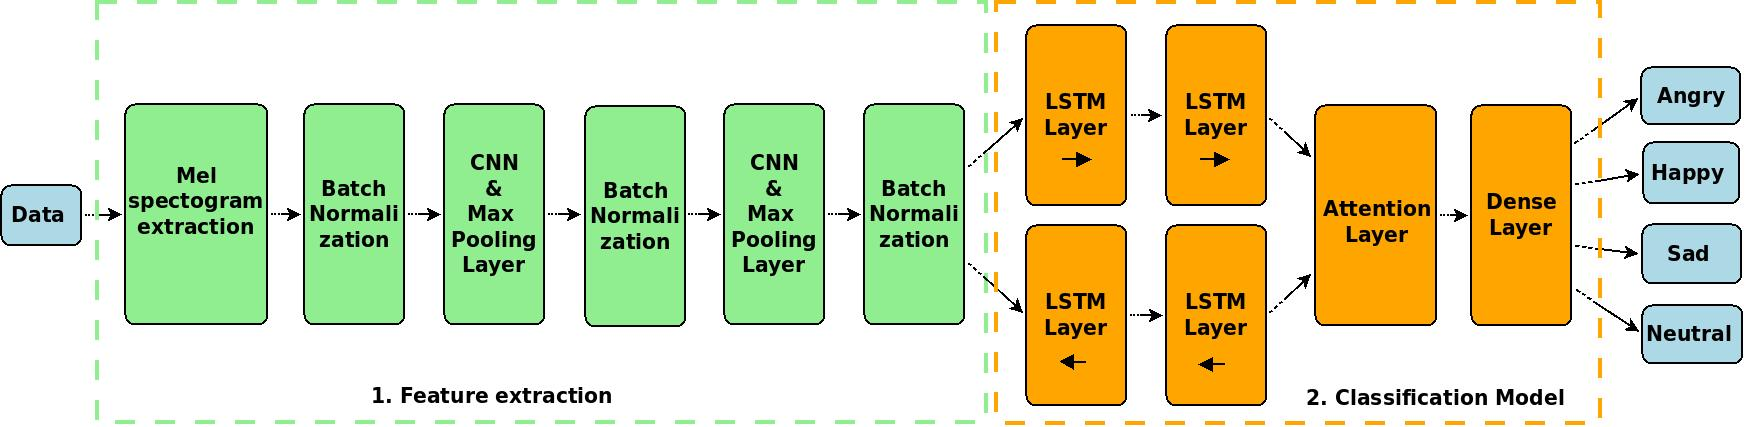
\includegraphics[scale=0.290]{Sistem_Diagram}
						\caption{Arhitectura propusa pentru sistemul de recunoastere a emotiilor, alcatuita din cele doua etape principale: extragerea caracteristicilor de intrare din semnalul audio (verde) si modelul clasificator. (portocaliu).}\stepcounter{Figcount}
						\label{fig:model}
						
					\end{figure}
				
					Datele de intrare folosite in aceasta lucrare provin dintr-un set de mai multe baze de date alcatuit din: 'EMO-DB', 'RAVDESS', 'EMOVO', 'MAV', 'ENTERFACE' si 'JL'. Similar cu motivatia prezentata la \ref{prez_multi_domain}, decizia folosirii unui numar ridicat de baze de date este bazata pe depasirea dezavantajului numarului scazut de exemple pentru antrenare specific domeniului SER, detaliata in 1.3.1. In acelasi timp deoarece semnalele autio sunt inregistrate in medii si limbi diferite, generalitatea modelului creste considerabil si face posibila inferenta pe inregistrari din afara acestor seturi de date. \par
					
					Extragerea caracteristicilor de intrare din semnalul audio este realizata atat in maniera "end-to-end" folosind o retea neuronala convolutionala, \ref{cnns} cat si in maniera "hand-crafted" folosind operatii matematice predefinite, \ref{hand-crafted}. Arhitectura propusa, Fig. \ref{fig:model}, foloseste extragerea "end-to-end" iar metoda "hand-crafted" este folosita doar ca un termen de comparatie si este prezenta doar in modul de utilizare pentru antrenare. Aceasta decize este bazata pe rezultatele promitatoare obtinute prin folosirea arhitecturilor "end-to-end"  in mai multe sisteme SER si pentru ca, dupa cum am mentionat anterior, nu s-a descoperit inca un set de caracteristici "hand-crafted" care sa cuprinda perfect informatia emotionala. Intre fiecare nivel ale retelei convolutionale am introdus tehnica numita "batch-normalization", \ref{batch-norn}, pentru a reduce fenomenul de expolize al gradientilor si a grabi procesul de antrenare. \par
					Structura interna a modulului clasificator ales a fost bazata pe rationamentul detaliat in Misramadi et al., 2017 \cite{misramadi}. Astfel, modelul clasificator este unul complex altcatuit din 3 componente: reteaua recurenta, mecanismul de atentie si reteaua neuronala densa, dupa cum se poate observa si in Fig. \ref{fig:model}.  
					Reteaua neuronala recurenta este consituita din doua celule recurente BLSTM ("Bidirectional Long Short-Term Memory") pe doua nivele. Aceasta tipologie de retea neuronala a fost aleasa pentru a profita de relatiile temporale ale informatiile emotionale dintre segmente audio aflate la diferite momente. Reteua recurenta este urmata de un mecanism de atentie care permite modelului sa se focuseze doar pe segmentele semnalului audio bogate in emotie. Reteaua neuronala generica densa este concatenata la modulul clasificator pentru a realiza translatarea rezultatelor retelei recurente si a mecanismului de atentie in distributia de probabilitate a emotiilor clasificate.\par
					
					Numarul de emotii clasificate este patru, la fel ca in arhitecturile din Misramadi et al., 2017 \cite{misramadi} si	Li, Yuanchao et al.2019 \cite{yuan}: fericire, tristete, enervare si neutru. \par
					
					Lucrarea contine si o interfata grafica care permite utilizatorului sa utilizeze sistemul de recunoasterea a emotiilor in vorbire descris mai sus printr-o gama larga de functionalitati. Interfata grafica permite doua moduri de utilizare: antrenare si inferenta. In partea de antrenare, utilizatorul poate sa modifice configuratia parametrilor modelului si sa observe diferite statistici legate de starea acestuia in timpul procesului de invatare. In modul de utilizare inferential, utilizatorul poate sa clasifice emotiile din fisiere audio pre-inregistrate sau din semnale inregistrate pe loc prin intermediul interfetei grafice.\par				
			\chapter{Bazele teoretice}
				 Domeniul inteligentei artificiale difera de oricare alta ramura a stiintei calculatoarelor deoarece isi propune sa rezolve problemele printr-o maniera stohastica. Avantajul privirii problemelor intr-un mod probabilistic este ca ne permite sa aplicam alogritmii obtinuiti direct pe lumea reala. Algoritmii clasici pot fi extrem de performanti cand vine vorba de a gasii solutii in timp polinomial, dar neputinciosi daca problema necesita solutii de un grad mai inalt de complexitate, timp exponential. Lumea in care traim este plina de astfel de probleme, iar abordarile clasice functioneaza doar pe difeirte abstractizari in care aspectele stohastice sunt eliminate aproape complet. \par				 
				 Metoda propusa de domeniul inteligentei artificiale este de a inlocui abordarea traditionala in care programatorul dicteaza pasii care duc la rezolvarea problemei cu un proces de antrenare prin care algorimtului ii sunt oferite doar un set de unelte pe care trebuie sa invete sa le foloseasca singur din greseli. \par			 
				 Recunoasterea emotiilor in vorbire face parte din multimea acestor probleme denumite "grele", putand deveni o sarcina dificila chiar si pentru oameni. Rezolvarea unei astfel de probleme poate fi realizata doar prin folosirea unei arhitecturi bazata pe inteligenta artificiala. Din acest motiv in urma studierii mai multor implementari prezentate in diferite articole stintifice din acest domeniu am decis sa construiesc un model de clasificare cu arhitectura din Fig. \ref{fig:model}. \par
				Dupa cum se poate observa in figura de mai sus, sistemul SER propus este alcatuit din doua parti principale: extragerea caracteristicilor de intrare si modelul clasificator. Fiecare din modulele care alcatuiesc aceste parti reprezinta decizii arhitecturale a caror motivatie teoretica si practica uremaza sa fie descrisa in sectiunile urmatoare. Deoarece exgragerea caracteristicile de intrare este realizata atat prin tehnica "hand-crafted" cat si "end-to-end", aspectele teoretice folosite de ambele metode vor fi descrise. Cu toate acestea, arhitectura propsa este cea "end-to-end", ilustrata in Fig. \ref{fig:model}.
			\section{Machine learning si retele neuronale artificiale} \label{ml}
				"Machine Learning"-ul este domeniul de studiu care ofera calculatoarelor abilitatea de a invata o sarcina fara sa fie explicit programate pentru a face acest lucru. " [Arthur Samule, 1959]  \par
			
			Era in care ne aflam este des numita "big data era", sugerand cantinatea imensa de informatii pe care omanirea o detine pentru prima data in istorie. In acelasi timp, tehnologia a evoluat pana in punctul in care putem sa cream alogritmi care sa se foloseasca de aceste informatii pentru a rezolva sarcini care pareau pana acum imposibil de rezolvat pentru algorimtii generici. "Machine Learning" este domeniul reprezentativ pentru acest tip de algoritmi, alcatuind un set de metode care pot detecta relatiile din interiorul datelor de intrare, si sa se foloseasca de aceste relatii invatate pentru a face predictii pe seturi de date noi. \par
			
			"Machine learning"-ul este structurat in patru mari tipuri de algoritmi: supervizati, nesupervizati, semi-supervizati si asa numitii "reinforcement learning algorithms". Proiectul meu este orientat pe gasirea unei solutii pentru recunoasterea emotiei din vorbire. Aceasta recunoastere se numeste in termeni tehnici \textit{clasificare}, si face parte din ramura algoritmilor supervizati pe care urmeaza sa ne axam in continuare. \par 
			Algoritmii supervizati trebuie sa faca o mapare de la un numar de intrari $X$ la un numar iesiri $y$ dupa ce au procesat un set de perechi $D={(x_i,y_i)}^N_{i=1}$, numit set de date de antrenare. Algoritmii supervizati sunt ghidati astfel sa gaseasca o solutie pentru o anumita problema printr-un set de exemple prin care li se prezinta un set de intrari si rezultatele dorite , conexiunea dintre intrare si iesire ramanand sa fie determinata de acestia printr-un proces de invatare din greseli. \par
			
			Termenul de "deep learning" se refera la o sub-diviziune a doemniului "Machine Learning", fiind specialzata pe folosirea retelelor neuronale profunde. Aceste retele neuronale sunt denumite profunde deoarece reprezina un set de functii, nivele, aranjate intr-un lant aciclic, Fig. \ref{fig:nns}. Primul nivel se numeste de obicei nivelul de intrare , nivelele din interiorul acestui lant se numesc "ascunse", iar nivelul de final se numeste nivel de iesire. Dupa cum se poate observa in Fig. \ref{fig:nns} fiecare din nivele unei retele neuronale este alcatuit la randul lui dintr-un numar de neuroni. Arhitectura unei retele neuronale este bazata pe conexiunile neuronale ale creierului, unde activarea unui neuron poate determina activarea unui alt neuron la care este conectat, obtinandu-se astfel o reactie in lant care are ca scop final realizarea unor procese complexe. 
			
			\begin{figure}[t]
			\centering
			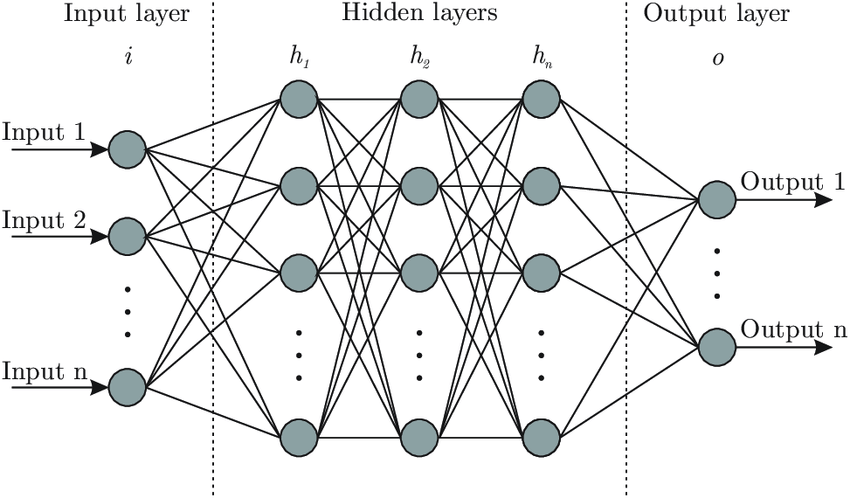
\includegraphics[scale=0.50]{nns}
			\caption{Structura interna a unei retele neuronale dense. Fiecare nod este conectat la toate nodurile din nivelele adiacente, iar intre nivelul de intrare si iesire exista un numar arbitrar de nivele "ascunse". Figura apartine articolului Facundo et al. (2017) \cite{nnspic}}
			\label{fig:nns}
			\end{figure}	

			Neuronii unei retele neuronale artificale generice sunt alcatuiti dintr-un set de ponderi care odata inmultite cu fiecare intrare si adunate cu un coeficent, numit "bias", genereaza la randul lor o intrare pentru neuronii umratori. 
			\noindent Iesirea fiecarui neuron este determinata dupa formula urmatoare:
			\begin{equation}
					a_j^{(i)} = \sum_{k=1}^{M} w_{jk}^{(i)} + w_{j0}^{(i)}
			\end{equation}
			
			unde $a_j^{(i)}$ reprezinta activarea neuronului $j$ din nivelul $i$, iar $w_{jk}^{(i)}$ si $w_{j0}^{(i)}$ reprezinta ponderile respective coeficientul "bias" al acelui neuron. \par
			
			Desi prin conectarea unor astfel de neuroni se pot obtine arhitecturi complicate, pentru ca o retea neuronala sa se poata sa aproximeze functii complexe fiecare din iesirile acestor neuroni trebuie sa fie urmate de o asa numita \textit{functie de activare}. Aceasta functie de activare are rolul de a elimina liniaritatea din interiorul retelei neuronale si sa mareasca astfel numarul gradelor de libertate. Fiecare nivel poate fi reprezentat printr-o matrice iar fiecare trecere prin acel nivel poate fi exprimata printr-o inmultire matriciala. Fara existenta acestor functii de activare reteaua neruonala ar fi doar un set de inmultiri matriciale, care la randul lui paote fi reprezentat ca o matrice unica, eliminand in sine sensul retelelor adanci. Din acest motiv activarea unui neuron devine $h_j^{(i)} = z(a_j^{(i)})$, unde $z$ este functia de activare aleasa. \par
			\noindent Unele dintre cele mai populare functii de activare sunt:
			\begin{itemize}
				\item \textit{Sigmoid},  $f(x) = \frac{1}{1+e^{-x}}$, care aduce valoarea lui $x$ in intervalul (0, 1)
				\begin{figure}[h]
					\centering
					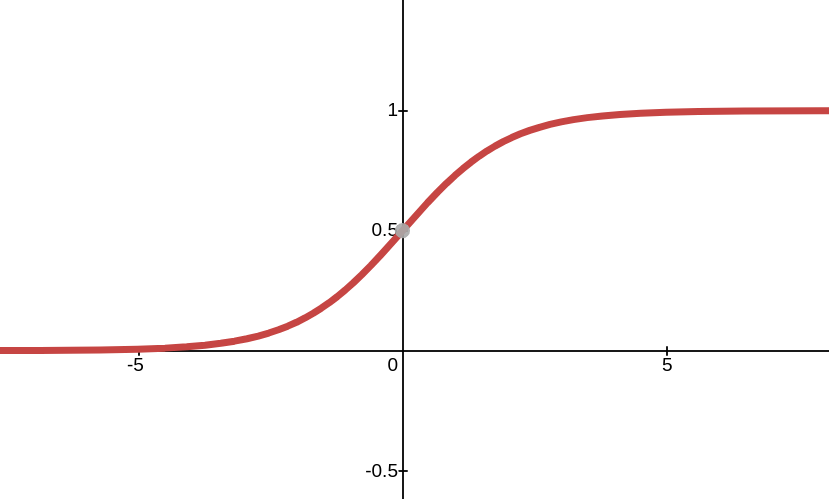
\includegraphics[scale=0.20]{sigmoid}
					\label{fig:nns}
				\end{figure}
				\newline	
				\item \textit{Tangenta hiperbolica},  $f(x) = \frac{(e^x-e^{-x})}{(e^x+e^{-x})}$, care aduce valoarea lui $x$ in intervalul (-1, 1)
				\begin{figure}[!h]
					\centering
					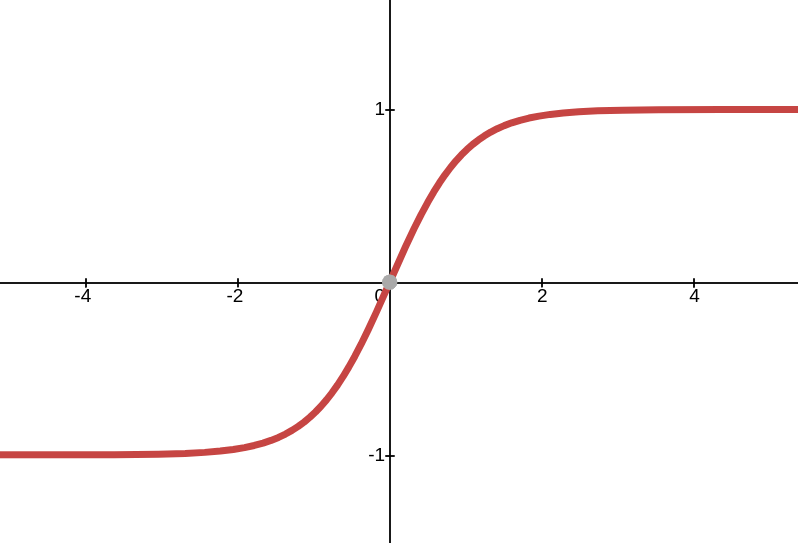
\includegraphics[scale=0.20]{tanh}
					\label{fig:nns}
				\end{figure}	
				\item \textit{ReLu}, $f(x) = \max(0, x)$, care aduce valoarea lui $x$ in intervalul  [0, $\inf$)
				\begin{figure}[!h]
					\centering
					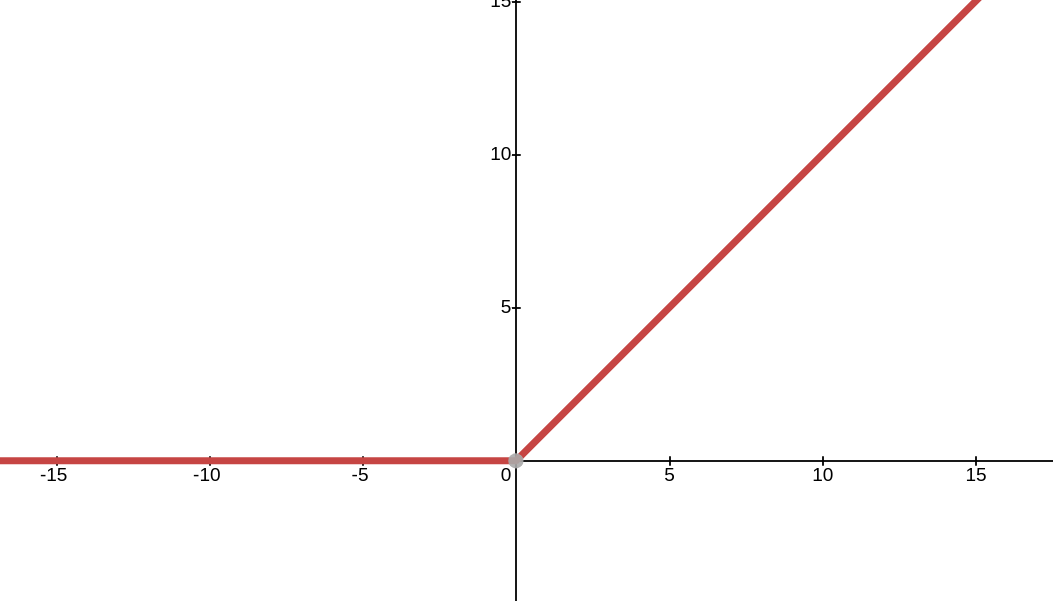
\includegraphics[scale=0.16]{relu}
					\label{fig:nns}
				\end{figure}	
				\item \textit{Leaky ReLu}, $f(x) = \max(0.01x, x)$, care aduce valoarea lui $x$ in intervalul  ($-\inf$, $\inf$)
				\begin{figure}[!h]
					\centering
					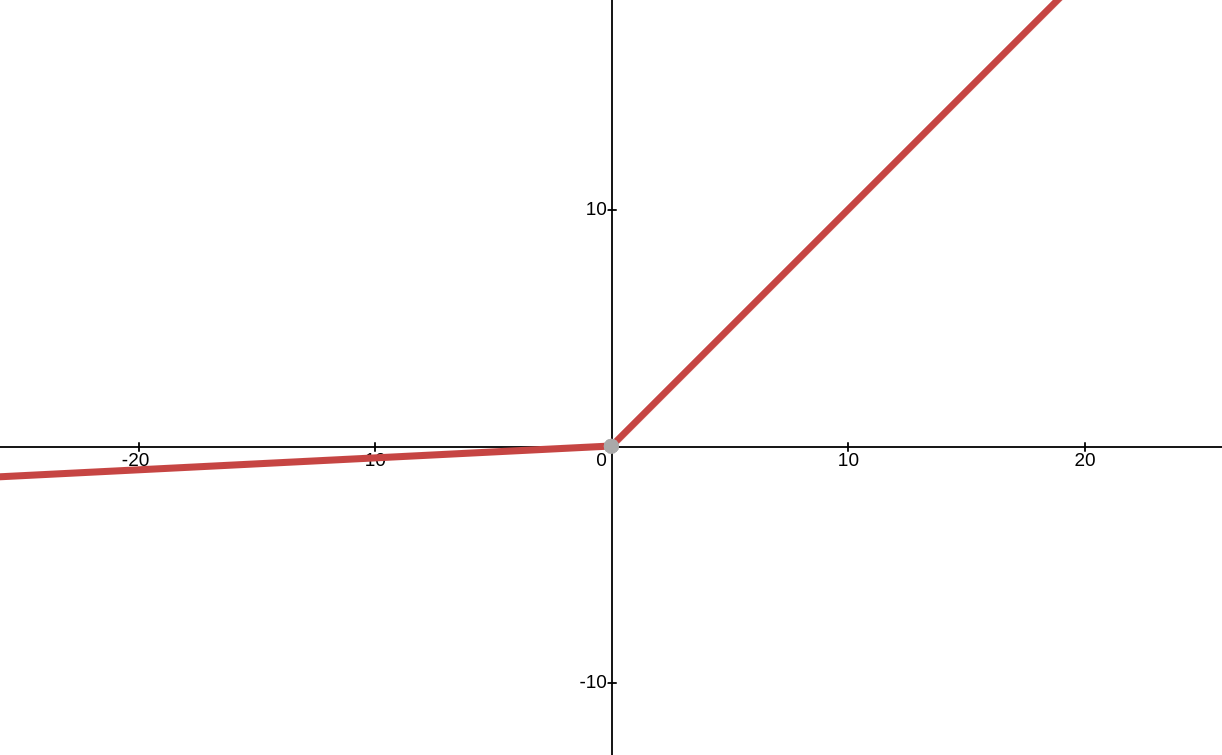
\includegraphics[scale=0.14]{lrelu}
					\label{fig:nns}
				\end{figure}
			\newpage
				\item \textit{ELu}, $f(x) = \max(\alpha (e^x -1), x)$, care aduce valoarea lui $x$ in intervalul ($-\inf$, $\inf$)
				\begin{figure}[!h]
					\centering
					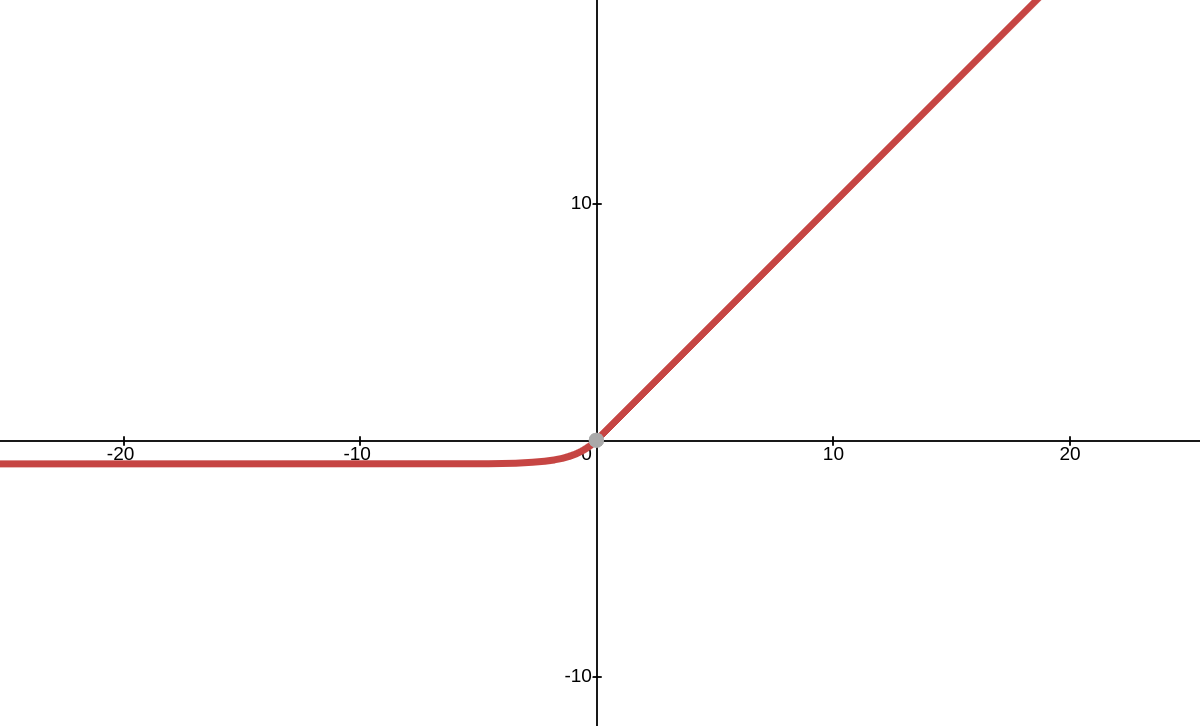
\includegraphics[scale=0.14]{elu}
					\label{fig:nns}
				\end{figure}	
			\end{itemize}
			\iffalse
			\begin{figure}[h]
				\begin{center}$
					\begin{array}{rr}
					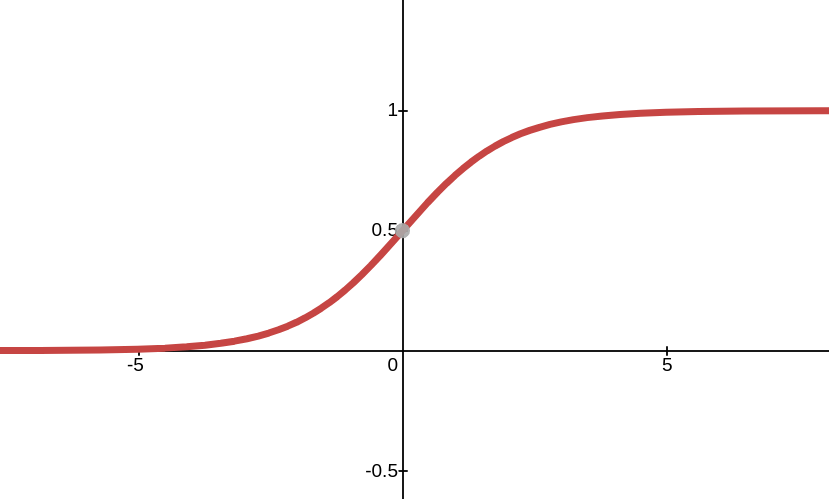
\includegraphics[scale=0.20]{sigmoid}&
					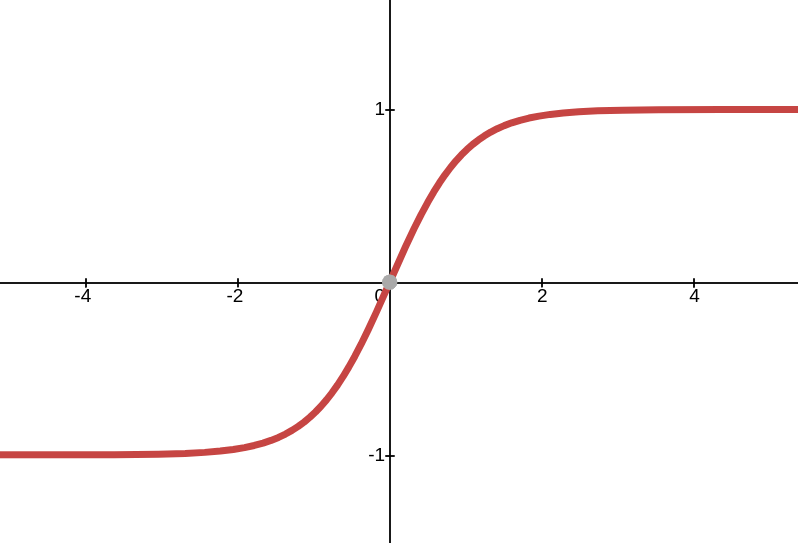
\includegraphics[scale=0.20]{tanh}
					\end{array}$
				\end{center}
				
				\begin{center}$
					\begin{array}{rr}
					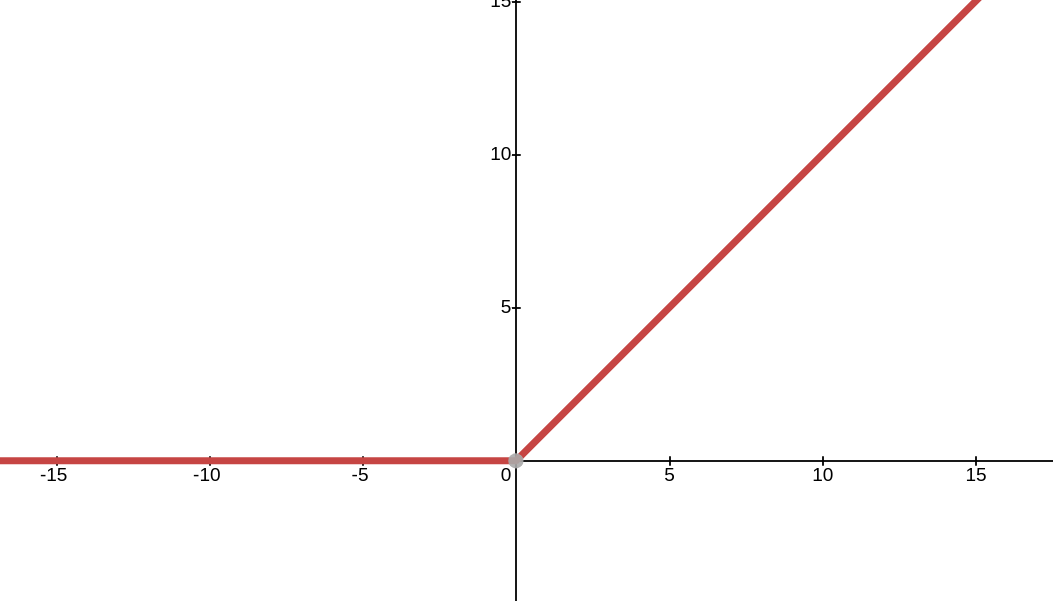
\includegraphics[scale=0.16]{relu}&
					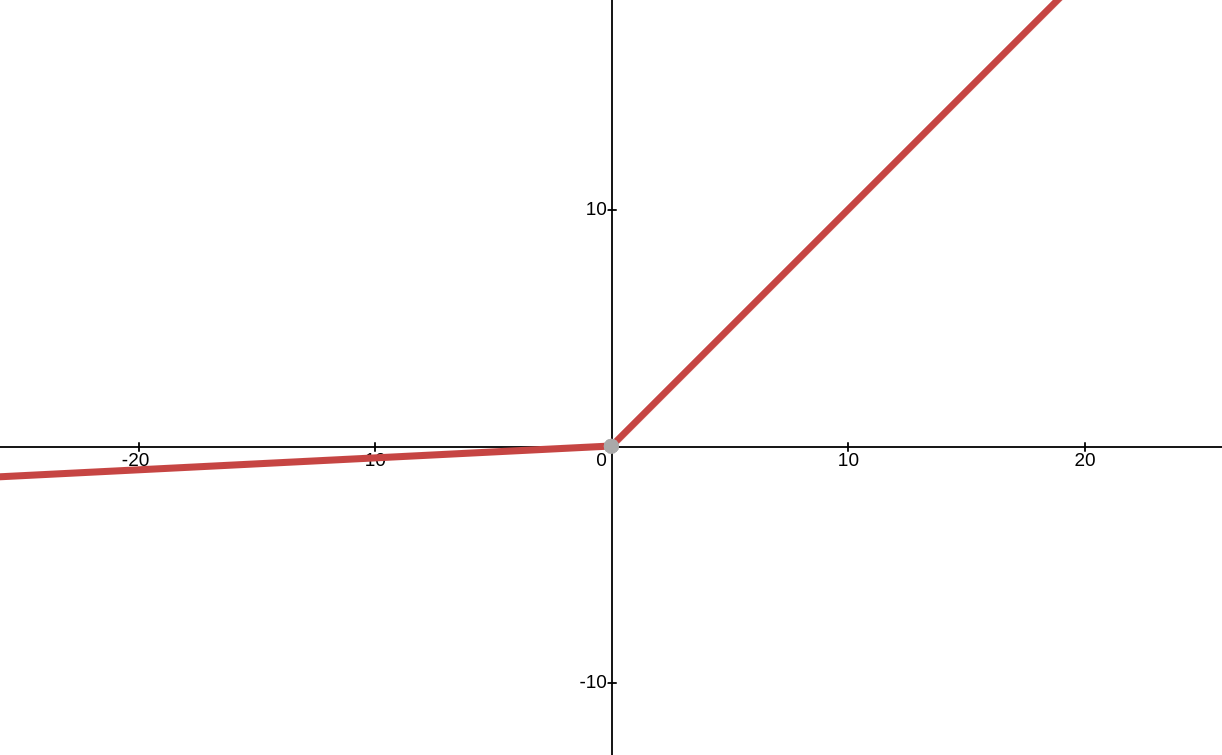
\includegraphics[scale=0.14]{lrelu}
					\end{array}$
					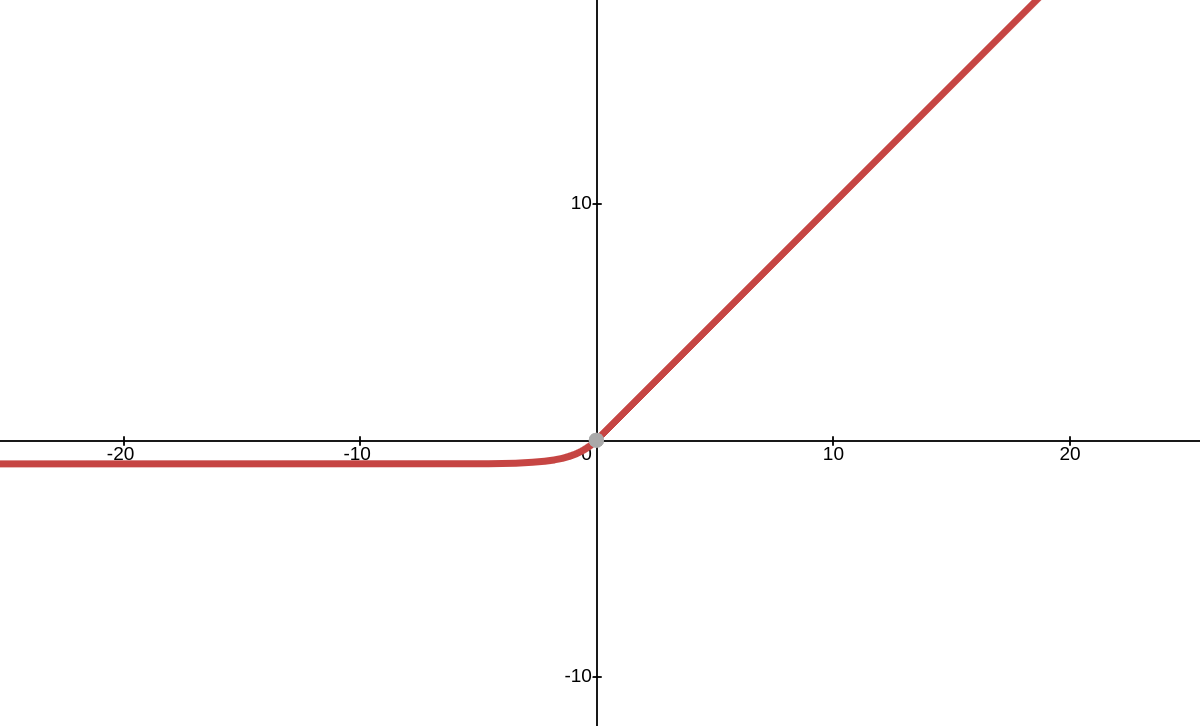
\includegraphics[scale=0.14]{elu}
				\end{center}
				\caption{Figure caption}
				\label{pics:blablabla}
			\end{figure}
			\fi
			In functie de problem pe care dorim sa o rezolvam, nivelul de iesire poate sa contina la randul lui o astfel de functie de activare. In cazul clasificarii binare este folosita functia sigmoid iar in cazul clasifiarii unui numar mai mare de clase de obicei se foloseste functia "cross-entropy". Pentru regresie, sau alte probleme care nu clasifica datele de intrare, nivelul final nu este urmat de o astfel de functie. \par
			
			Antrenarea retelelor neuronale se realizaza prin folosirea unor algoritmi numiti optimizatori. Acestia determina influenta pe care fiecare pondere din retea a avut-o asupra rezultatului final extragand derivata ponderii in raport cu eroare totala a retelei. Daca acea influenta a fost mare ponderea este modificata puternic, in caz contrar aceasta este modificat putin. Prin folosirea unui numar mare de astfel de exemple ponderile ajunga sa convearga la un set de valori care permit aproximarea unei multitudini de functii complexe. \par
			
			Functia de calcul a erorii poate avea forme diferite, dar una din cele mai folosite este eroarea patratica medie \ref{rms}.
			\begin{equation} \label{rms}
				E(W) = \frac{1}{2} \sum_{n=1}^{N} (y(x_n, W) - t_n)^2
			\end{equation}
			unde $E(W)$ este eroarea calculata, $N$ reprezinta numarul total de exemple de antrenare, $y(x_n, W)$ este predicia pentru exemplul cu numarul $n$ iar $t_n$ este valoarea adevarata. \par
			
			Recunoasterea emotiei in vorbire este o problema de clasificare. In acest caz, $y(x_n, W)$ reprezinta o distributie de probabilitate asupra emotiilor estimata de model iar $t_n$ este un vector de forma $[0,1,0,0]$, in care valoarea $1$ este pe pozitia emotiei aferente acelui exemplu. \par
			
			In arhitectura acestui proiect am folosita mai multe tipuri de retele neruonale pentru indeplinirea mai multor functionalitati. Aceste tipologii si modul lor de utilizare urmeaza sa fie descrise in detaliu in sub-capitolele urmatoare.
			\section{Transformata Fourier discreta pe timp scurt} 
			
			Orice forma de unda, indiferent daca e observata in univers sau mazgalita de noi pe foaie, reprezinta de fapt doar o suma de functii sinusoidale de diferite frecvente.\par
			
			Un semnal audio este un semnal complex alcatuit din mai multe unde de diferite frecvente care circula sub forma unor perturbatii prin mediu. Atunci cand inregistram un semnal audio capturam doar amplitudinile rezultate in urma combinarii acestor unde. Transformata Fourier este un concept matematic care ne permite sa descompunem un semnal in frecventele care il compun si magnitudinile acestora.\par 
			
			Motivul folosirii transformatei Fourier vine de la studiul seriilor Fourier. Prin studiul acestor serii, funcții periodice complicate sunt scrise ca simple sume de unde reprezentate matematic prin funcțiile sinus și cosinus.\par
			
			Fie o functie periodica $f(t)$, cu o perioada fundamentala $T$, aceasta are aferenta seria Fourier urmatoare:
			\begin{equation}
				g(t) = a_0 + \sum_{m=1}^{\infty} a_m \cos(\frac{2\pi m t}{T}) + \sum_{n=1}^{\infty} b_n \sin(\frac{2\pi n t}{T})
			\end{equation}			
			unde $a_0$, $a_m$ si $b_n$ sunt coeficientii Fourier calculati sub forma			 
			\begin{align}
			\nonumber 	a_0 &= \frac{1}{T} \int_{0}^{T} f(t) dt\\
			\nonumber 	a_m &= \frac{2}{T} \int_{0}^{T} f(t) \cos(\frac{2 \pi m t}{T}) dt \\ 
						b_n &= \frac{2}{T} \int_{0}^{T} f(t) \sin(\frac{2 \pi n t}{T}) dt \label{coef_fr}
			\end{align}
			Aceste relatii pot fi scrise intr-o forma mai eleganta din punct de vedere matematic prin folosirea numerelor complexe, si mai exact a formulei lui Euler,  \(\mathrm{e}^{2\pi i\theta} = \cos (2\pi \theta) + i \sin (2\pi \theta)\).			
			\begin{equation} \label{cmpl_frs}
				g(t) = \sum_{n=-\infty}^{\infty} c_n  \mathrm{e}^{i \frac{2\pi n t}{T}} 
			\end{equation}
			unde $c_n$ reprezinta echivalentul coeficientiilor Fourier $a_m$ si $b_n$ din \ref{coef_fr}			
			\begin{equation*}
			 	c_n = \frac{1}{T} \int_{0}^{T} f(t) \mathrm{e}^{-i \frac{2\pi n t}{T}} dt
			\end{equation*}
			
			Transformata Fourier este o operație care se aplică unei funcții complexe și produce o altă funcție complexă care conține aceeași informație ca funcția originală, dar reorganizată după frecvențele componente. Transforamta Fourier este o generalizare a seriilor Fourier complexe prezentate in \ref{cmpl_frs}, putand fi vazuta ca limita seriei Fourier cand perioada tinde la infinit.
				
			Fie $f : R \to C$ absolut integrabila. Functia complexa de variabila reala	$F : R \to C$,
			\begin{equation*}
						F(\omega) = \int_{-\infty}^{\infty}  \mathrm{e}^{-2\pi i\omega t} f(t) dt
			\end{equation*}
				se numeste transformata Fourier a functiei f, iar
			
			\begin{equation*}
				f(t) = \int_{-\infty}^{\infty}  \mathrm{e}^{2\pi i\omega t} F(\omega) d\alpha
			\end{equation*}
				se nu meste inversa tranformatei Fourier. \par
			Astfel transformata Fourier reprezina o unealta care ne permite sa schimbam unghiul din care privim diferitele semnale de tip unda, facand posibila trecerea din domeniul temporal in domeniul frecventa Fig.\ref{fig:tf}. Acest domeniu ne permite sa diferentiem intre semnalele de diferite frecvente care alcatuiesc unda. Prin folosirea inversei transformatei Fourier, putem chiar sa eliminam anumite semnale prin modificarea coeficientiilor aferenti frecventelor acestora. Acest concept a deschis granitile unei arii uriase de aplicatii ale acestei teoreme, fiind revolutionara pentru domeniul procesarii semnalelor.  	
				\begin{figure}[h]
					\centering
					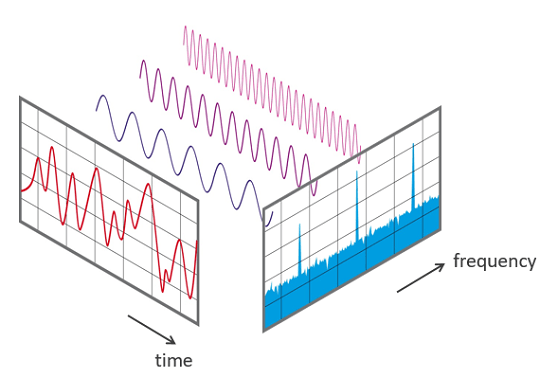
\includegraphics[scale=0.50]{ft}
					\caption{Ilustrare grafica a translatarii semnalului audio in domeniul frecventa dupa aplicarea transformatei Fourier. Figura apartine paginii web din Trekhleb, 2018 \cite{stft6}.}
					\label{fig:tf}
				\end{figure}		
				
			"Short-time Fourier transform", sau STFT, este o varianta a transformatei Fourier prezentata mai sus, folosita pentru a determina frecventele sinusoidale si magnitudinile unor sectiuni locale dintr-un semnal. In practica, procedura prin care se calculeaza functiile STFT este de a impartii semnalul temporal in segmente mai mici de dimensiuni egale si apoi de a calcula transformata Fourier pe fiecare din aceste segmente separat. 
			\begin{equation*}
			STFT(r , \omega) = \int_{-\infty}^{\infty}  f(t) w(t-r)\mathrm{e}^{- i 2\pi \omega t}  dt
			\end{equation*}
			unde w(r) este o functie fereastra. \par
			STFT ofera informatii asupra frecventei pe un anumit interval temporal local, fiind folosita in situatii in care frecventele componente ale unui semnal variaza puternic in timp. Transformata Fourier in schimb ofera doar media informatiilor frecventelor pe intregul interval de timp al semnalului \cite{stft2}.
			
			Deoarece semnalul audio este discretizat si segmentat, in procesarea acestuia se foloseste varianta discreta a STFT.
			
			\begin{equation}
			STFT(m ,\omega) = \sum_{n=-\infty}^{\infty}  f[n] w[n-m]\mathrm{e}^{- i 2\pi \omega n}  \label{stft}
			\end{equation}
			
			
			\section{Hand-crafted features} \label{hand-crafted}
			
			Metoda "hand-crafted" de extrage a caracteristicilor de intrare din semnalul audio este bazata pe diferite formule matematice. Dupa cum am spus si in sub-capitolul 1.3, momentan nu exista un set de caracteristici reprezentative pentru informatia emotionala, iar majoritatea implementarilor aleg aceste caracteristici printr-o selectie empirica. Majoriatea caracteristicilor fiind importate din problema recunoasterii informatiei lingivstice din vorbire, "Speech Recognition". \par
			
			Chiar daca alegerea setului de caracteristici este subiectiva fiecarei implementari, majoritatea impartasesc un set restrans care se considera ca surprinde anumite informatii din discursul uman. Coeficientii Mel cepstrali si functile delta si delta-delta ale acestora fac de obicei parte din datele de intrare a sistemelor SER "hand-crafted" si din cauza populariatii acestora urmeaza sa le descriu in continuare. \par
			
			\subsection{Coeficientii Mel cepstrali}
				Coeficientii Mel cepstrali, sau MFCC, sunt cea mai folosita reprezentare a prorietatiilor spectrale ale semnalelor vocale. Acestia functioneaza cel mai bine in cazul domeniului "Speech Recognition" deoarece iau in calcul senzitivitatea perceptiei umane in interpretarea frecventelor prezente in semnalul audio. Pentru calcularea acestor coeficienti, trebuie sa urmam o serie de pasi \cite{mcs}.
					\begin{enumerate}
						\item 
							In primul rand se calculeaza o estimare a denistatii spectrale a semnalului, asa numite "Periodogram estimate of the power spectrum". Pentru calcularea acesteia se aplica transformata Fourier pe termen scurt \ref{stft} pe fiecare segment din semnalul audio. Odata obtinut echivaletul semnalului audio in domeniul frecventa , numit "complex spectrum", se ridica la patrat valoarea absoluta a acesteia pentru obtinerea "Periodogram"-ei.
							\begin{equation*}
								P_i(k) =\frac{1}{N}\mid STFT(i, k)\mid^2 \quad\quad,1\leq k\leq K
							\end{equation*}
							unde $i$ este numarul segmentului actual, $N$ este numarul total de segmente audio si $K$ este frecventa maxima, sau "lungimea transformatei Fourier discrete".
						\item Urmatorul pas este aplicarea asa-ziselor "Mel filerbanks". "Mel filerbanks" sunt filtre triunghiulare care au valori nule pe majoritatea lungimii spectrum-ului. Aceste filtre se calculeaza prin scalarea unor frecvente alese la distante egale dintr-un interval, de obicei $[300Hz, 8000Hz]$, in scara Mel. Aceasta scara reprezinta limitele capacitatii umane de percepere a diferitelor frecvente sonore. Scalarea frecventelor se realizeaza prin formula $M(f) = 1125 \ln(1+ f/700)$. Oamenii sunt mult mai buni in a diferentia schimbari la frecvente mici fata de frecvente inalte, iar prin incorporarea aceste scalari caracteristicile obtinute vor fi mult mai apropiate de ce ar auzi defapt un om. \newline
						Dupa ce s-a aplicat complet scalare Mel se creaza filtrele triunghiulare folosint urmatoarea formula
						\begin{equation*}
							H_m(k) = 
							\begin{cases}
							\quad \quad 0&\quad k<f(m-1) \\[3pt]
							\frac{k-f(m-1)}{f(m) - f(m-1)}&\quad f(m-1)\leq k\leq f(m) \\[5pt]
							\frac{f(m+1)-k}{f(m+1) - f(m)}&\quad f(m)\leq k\leq f(m+1) \\[3pt]
							\quad \quad 0&\quad k>f(m+1)
							\end{cases}
						\end{equation*}
						unde $m$ este numarul frecventei scalate, iar $k$ este frecventa curenta din spectrum. \newline
						Filtrele triunghiulare sunt inmultite apoi cu "power spectrum"-ul obtinut la pasul anterior si se obtin astfel energiile din fiecare filtru Mel.
						\item Urmatorul pas reprezinta logaritmarea acestor energi.
						\item Ultimul pas fiind aplicarea transforamtei cosinus discreta (DCT). Motivatia acestui pas este ca energiile obtinute anterior au un grad ridicat de corelatie iar aplicarea DCT realizeaza decorelara lor si ofera reprezentarea compresata a acestora.
						Formula pentru DCT fiind,
						\begin{equation*}
							X_k = \frac{1}{2}(x_0 + (-1)^k x_{N-1}) + \sum_{n=1}^{N-2} x_n cos[\frac{\pi}{N-1}nk]
						\end{equation*}
						Amplitudinile spectrum-ului rezultat reprezinta coeficientii Mel cepstrali.
				\end{enumerate} \par
				\subsection{Deltas si delta-deltas}
					Totusi, coeficientii Mel descriu doar coperta puterii spectrale a fiecarui segment din semnalul audio, dar s-a demonstrat empiric ca o parte importanta din informatia vocala se afla si in spatele dinamicii acestor coeficienti. Acest lucru se calculeaza folosind caracteristicile delta si delta-deltas. \par
					Coeficientii deltas sunt calculati din MFCC prin urmatoarea formula:
					\begin{equation*}
						d_t = \frac{\sum_{n=1}^{N} n(c_{t+n}-c{t-n})}{2\sum_{n=1}^{N}n^2}
					\end{equation*}
					unde $d_t$ reprezinta coeficientul delta, din segmentul $t$  in functie de coeficientii statici $c_{t+n}$ si $c_{t-n}$. 
					Coeficientii delta-delta sunt calculati prin aceeasi formula, inlocuindu-se doar coeficentii MFCC cu cei delta. \par
				
				Pe langa acesti coeficienti, caracteristicile "hand-crafted" pot contine si urmatoarele: tonalitate, probabilitate vocala, energie,  radicalul mediei amplitudinii la patrat, rata zero-crossing, chroma, coeficientul rollof, ratia harmonics-to-noise, bruiajul, media, variatia, minimul si maximul semnalului audio etc. Toate acestea se calculeaza cu functii matematice predefinite asemanatoare cu procesul de obtinere a coeficentiilor MFCC.			
				
				In implementarea extragerii caracteristicilor "hand-crafted" folosita de mine am folosit: MFCC, delta, delta-deltas, radicalul mediei la patrat a amplitudinii fiecarui segment, rata zero-crossing, chroma si coeficientul rollof.
				
			\section{End-to-end feature extraction}	\label{end-to-end}
			
			Avansarile recente ale algoritmilor si a hardware-ului calculatoarelor au facut posibila antrenarea retelelor neuronale intr-o maniera end-to-end pentru sarcini care necesitau in trecut expertiza umana. Pe langa ca aceste arhitecturi de retele solicita mai putin efortul uman decat abordarile traditionale, in general acestea obtin si performante superioare. Acest aspect este in mod particular adevarat atunci cand cantitatea de date pentru antrenare disponibila este mare, deoarece beneficiile optimizarii holistice tinde sa depaseasca acelea a cunostintelor anterioare  \cite{graves}. \par
			
			Arhitectura "end-to-end" este preazentata in Fig. \ref{fig:model}. Dupa cum poate fi observat, extragerea caracteristicilor in aceaast arhitectura este realizata prin atasarea unei retele convolutionale  combinata cu o tehnica de normalizare intre fiecare nivel. Aceste retele convolutionale sunt celebre pentru procesarea imaginilor pentru ca, spre deosebire de retelele neuroanle artificiale normale, se folosesc de relatiile spatiale bidimensionale dintre pixeli. Astfel pentru a ne folosi de acest avantaj se extrage spectograma Mel a semnalului audio, care va fi folosita ca date de intrare pentru aceste retele. Un exemplu al unei astfel de spectograme se poate observa in Fig. \ref{fig:melspec}. \par
						
			\begin{figure}[h]
				\centering
				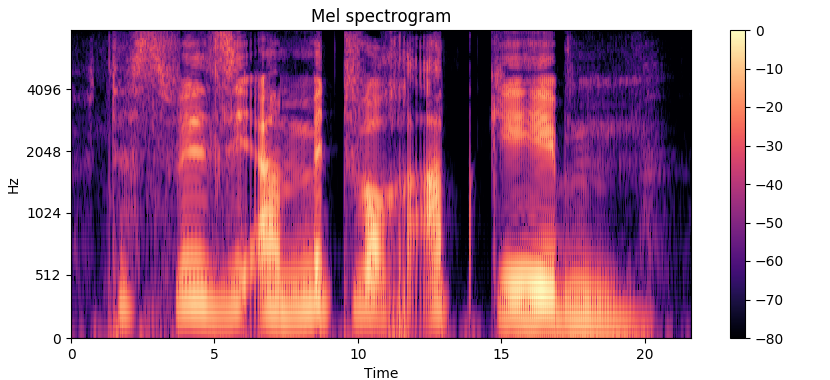
\includegraphics[scale=0.67]{melspectogram}
				\caption{Spectograma Mel a unui semnal audio extras cu ajutor librarie librosa \cite{librosa}. Spectograma ilustreaza valoarea amplitudinilor frecventelor din fiecare moment al semnalului audio.}
				\label{fig:melspec}
			\end{figure}
			
			\subsection{Spectograma Mel} \label{mel}
				Prin spectograma se intelege reprezentarea vizuala a unui spectrum de frecvente a unui semnal in raport cu timpul. Astfel intr-o spectograma, o axa reprezinta , alta reprezinta timpul iar intensitatea culorii reprezitna magnitudinrea(amplitudinea) frecventei observate la acel moment din timp. Calcularea spectogrameleor Mel este extrem de asemanatoare cu calcularea coeficientilor de corelati Mel prezentati in sub-sub-capitolul 3.1.2. Astfel pasii 1, 2, si 3, prezentati anterior, se reproduc. Singura diferenta este in loc de calcularea transformatei cosinus discreta si extragerea coeficientilor ca la pasul 4, evoulutia valorile amplitudinii frecventelor in functie de timp sunt translatate intr-o matrice care va alcatuii spectograma. \par
			\subsection{Batch normalization} \label{batch-norn}
				Unul din motivele pentru care antrenarea retelelor neuronale profunde, cu mai multe nivele, devine dificila este faptul ca distributia intrarilor fiecarui nivel se schimba in timpul antrenarii, prin modificarea parametrilor nivelului anterior care le genereaza. Acest lucru incetineste drastic procesul de invatare al modelului deoarece alegerea modului de initializare a parametrilor capata un impact mult mai ridica si face necesara alegerea unor rate de antrenare mai mici. Acest fenomen se numeste "internal covariate shift", iar o solutie propusa de Ioffe \& Szegedy et al., 2015 \cite{batch_norm}, este normalizarea intrarilor fiecarui nivel. \par
				Formula pentru normalizare este cea generica:
				\begin{equation*}
					x'_i = \frac{x_i - \mu_B}{\sqrt{\sigma^2_B +  \varepsilon}}
				\end{equation*}
				
				\quad unde $x_i$ reprezinta intrarea cu numarul i, $\mu$ este media setului de intrari al nivelului curent, $\sigma$ este deviata standard a acestor intrari iar $\epsilon$ reprezinta doar o constanta pentru a evita impartirea la 0.
				
				Pe langa reducerea fenomenului prezentat anterior, "internal covaraite shift", aceast mecanism de normalizare aduce alte doua mari beneficii. In timpul antrenarii gradienti circula de la nivelul final al retelei spre inceput modificand parametrii modelului pentru a reduce eroarea inregistrata.
				Prin folosirea noramizarii inainte de fiecare nivel se reduce dependenta acestor gradienti de scala ponderilor nivelelor si de valoarea lor initiala. Acest lucru ne permite sa folosim rate de antrenare mai mari fara a pune in pericol convergenta modelului. \par
				Cel de al doilea avantaj este ca s-a demonstrat empiric \cite{batch_norm} ca tehnica "batch normalization" imbunatateste regularizarea parametrilor si marirea generalitatii modelului. \par
				Modelel SER sunt succeptibile la un fenomen denumit "explozia gradientiilor", deoarece folsoesc arhitecturi complexe cu un numar mare de parametrii. Pe langa acest considerent, acuratetea acestor modele depinde puternic de variabile greu de controlat ca modul de inregistrare a bazelor de date, locatia unde s-a desfasurat inregistrarea, multitudiea de vorbitori, diferentele de exprimare si a limbilor. "Batch normalizaton", ofera beneficii in ambele privinte deoarce functioneaza ca un regularizator, incetinind "exploziile" din interiorul nivelelor, si normalizeaza datele de intrare reducand astfel influenta diferentelor de la o inregistrare la alta. \par
			\subsection{Retele neurononale convolutionale} \label{cnns}
				Retelele neuronale convolutionale, sau CNN, reprezitna o adaptare a retelelor neuronale artificiale generice pentru rezolvarea sarcinilor vizuale, sau in care datele de intrare sunt organizate in doua dimensiuni. Desi aceste tipuri de retele neuronale au fost introduse prima data in 1989 ((Le Cun et al., 1989 \cite{leCun}), au crescut in popularitate abia in ultimii ani, dominand astazi majoritatea solutiilor propuse pentru diferitele sarcini din domeniul vizual. \par 
				
				Conceptul principal din spatele acestor arhitecturi reprezinta operatia matematica numita \textit{convolutie}, dupa care a si fost numita aceasta tipologie de retea neronala. Convolutia reprezitna o operatie care primeste ca intrari doua functii si reprezinta modul in care una dintre fucntii isi modifica forma in functie de cea de a doua functie.
				Formula unei convolutii discrete este urmatoarea:
				\begin{equation*}
					s(t) = (f*g)(t) = \sum_{n=-\infty}^{\infty} f(n) \cdot g(t - n)
				\end{equation*}	\par
				\noindent sau in doua dimensiuni
				\begin{equation}\label{convo}				
					S(i, j) = (I*K)(i, j) = \sum_{m} \sum_{n} K(m, n) \cdot I(i - m, j - n)
				\end{equation}
				
				Bazata pe aceasta formula matematica relativ simpla retele neuronale convlutionale au reusit sa depaseasca unele dintre principalele piedici pe care retelele neuronale simple le intalneau in procesarea imaginilor. Retele neuronale traditionale creaza conexiuni intre fiecare unitate de intrare si fiecare neuron din nivelul aferent. Avand un numar satisfacator de date de intrare acestea pot sa invete sa rezolve diferite sarcini care par imposibile pentru alogiritmii generici din stinta calculatoarelor. Totusi, dimensiuniea acestor arhitecturi poate creste extrem de rapid, iar pentru probleme ca procesarea imaginilor, unde diferite imagin pot avea sute de mii de pixeli, depasesc rapid capacitatile de procesare disponibile. \par
				Pe langa acest dezavantaj, arhitecturile generice nu reusesc sa suprinda esenta procesararii de imagini, sau a mecanismului de vedere uman, care este bazat pe conceptul ca pixelii care se afla in vecinataea unui anumit pixel sunt mult mai puternic corelati cu acesta decat oricare alti pixeli. Astfel desi aceste nivele din retelele neuronale generice se folosesc de intreaga informatie de intrare raman inflexibile cand vine vorba de a determina anumite linii, curbe sau forme ale obiectelor observate, ele luand in considerare doar intensitatea culorii unui pixel dintr-o locatie data. \par
				
				Retelele neuronale convolutionale reusesc sa treaca peste aceste obstacole prin folosirea a trei idei care au adus multe beneficii si in alte tipologii de retele neuronale,\textit{ filtre de receptie locale}, \textit{refolosirea parametriilor} si \textit{subesantionare}. \par
			
				Metodele traditionale de antrenare folosesc inmultirea matriciala intre intregul set de date de intrare si intregul set de parametrii dintr-un nivel. In schimb, CNN se folsoesc de asa numite \textit{filtre}, sau \textit{"kernels"}, care reprezinta un set de paramterii de dimensiuni de cateva ori mai mici decat datele de intrare. Aceste filtre sunt apoi inmultite doar cu anumite pari echivalente dimensional din datele de intrare. Astfel, de exmplu avand o imagine in dimensiuni 28x28 si un filtru de dimensiuni 3x3, acest filtru este aplicat pe bucati de dimensiuni 3x3 din matricea intrarilor plimbandul pe intreaga suprafata a imaginii. Rezultatul obtinut devine una din intrarile unui filtru urmator. Acest mecanism poate fi observat in Fig. \ref{fig:cnns}.
					
				\begin{figure}[h]
					\centering
					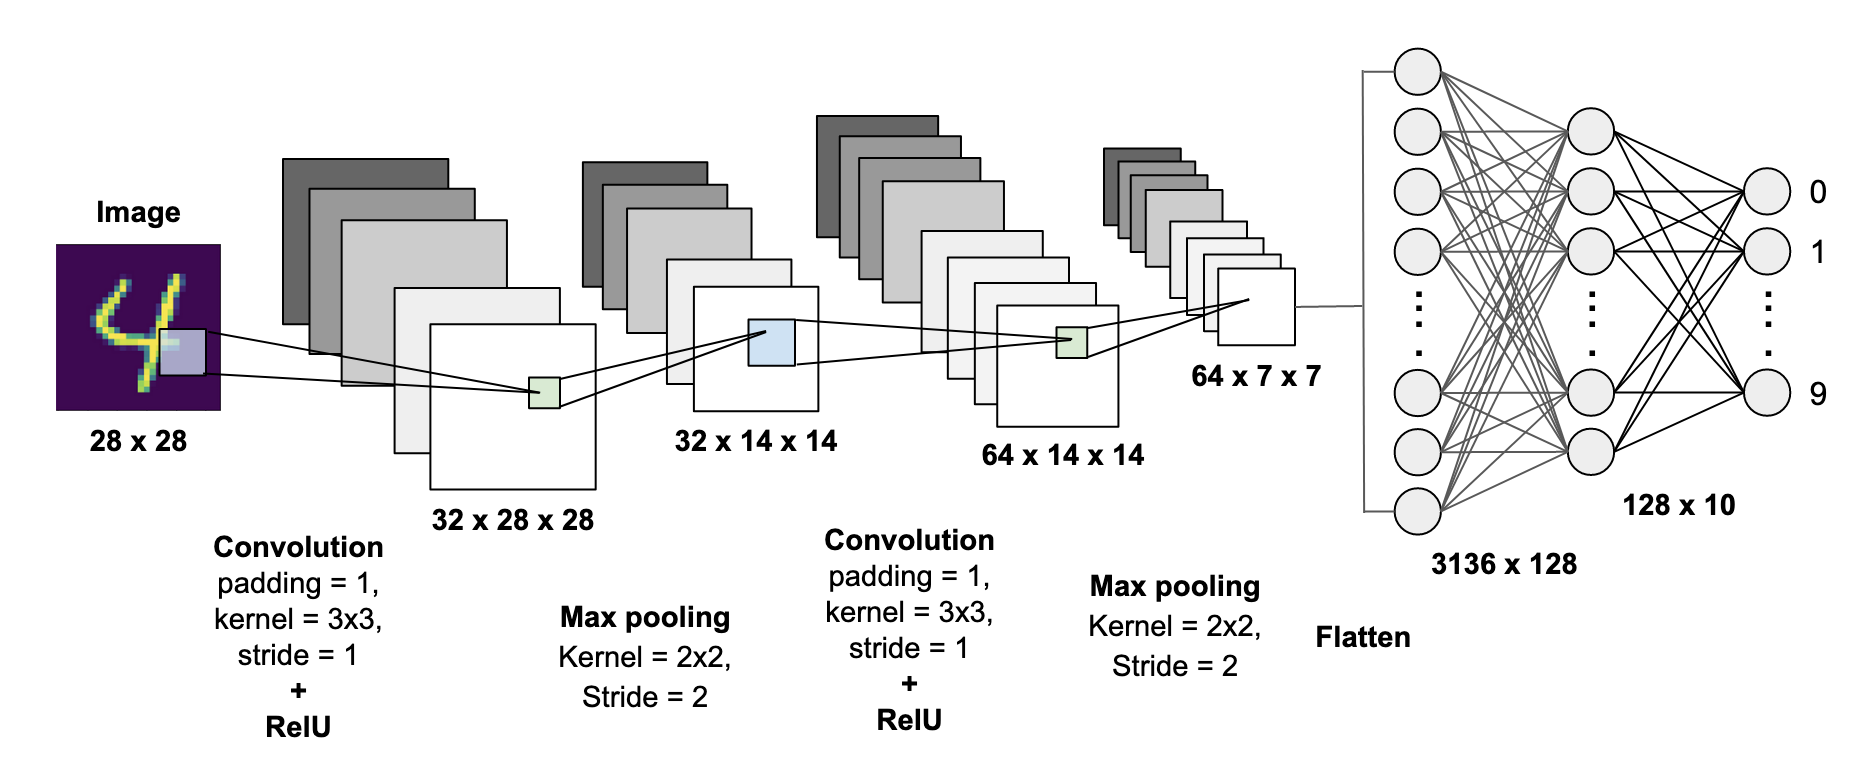
\includegraphics[scale=0.23]{cnns}
					\caption{Arhitectura unei retele neuronale convolutionale specialziata pe recunoasterea cifrelor scrise de mana. Figura apartine paginii din Patel, 2019 \cite{cnn_photo}}
					\label{fig:cnns}
				\end{figure}
				
				Simpla folosire a acestor filtre de dimensiuni reduse rezovla majoritatea problemlor impuse de arhitecturile traditionale. In primul rand prin acest mod reteaua neuronala primeste capacitatea de a determina caracteristici abstracte. Acest lucru este posibil prin faptul ca filtrele se focuseaza pe determinarea relatiilor din pixelii invecinati. In timpul antrenarii aceste filtre vor invata sa detemine anumite caracteristici din interiorul imaginilor. Deoarece acestia sunt aplicati succesiv pe intreaga imagine de intrare, ei o sa determine existenta si pozitia acelor caracteristici oriunde in matricea de intrare. Nivelele de la baza retelei invata sa determine caracteristici simple ca diferite puncte, linii sau curbe din diferite locatii ale imaginii, in timp ce nivelele de la capatul retelei prin combinarea informatiei de la filtrele anterioare ajung sa determine carcateristici complexe, ca diferite forme sau obiecte. Operatia de convoluie, \ref{convo}, prezinta perfect modul de aplicare al acestor filtre unde $I$ reprezinta imaginea iar $K$ filtrul aplicat pe fiecare portiune din acea imagine.\par
				
				Folisrea acestor filtre aduce si un mare avantaj din punct de vedere computational. Deoarece intre nivelele retelei si intrarile acestora nu mai exista conexiuni intre fiecare unitate si deoarece o pondere, "weight", nu este inmultita doar cu un singur element de intrare ci este refolosit de un filtru pentru intreaga imagine, numarul parametriilor folositi scade considerabil. Acest lucru reduce cerintele de memorie, creste eficienta statistica si ne permite sa folosim arhitecturi mai complexe in numarul de filtre aplicate. \par
				
				Odata ce aplicarea filtrelor s-a finalizat, rezultatul este de obicei transformat prin folosirea unuei functii de subesantionare. Cu ajutorul unor operatii matematice ca maximul, media, mediana etc., se realizeaza extragerea unui singur element dintr-un grup de pixeli invecinati, Fig \ref{fig:maxpool} . Daca este foloista functia de maxim acest mecanismt se numeste "Max-pooling".
								
				\begin{figure}[h]
					\centering
					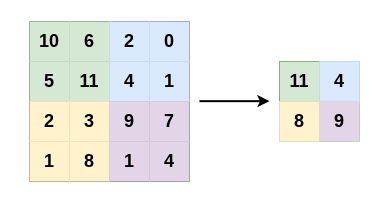
\includegraphics[scale=0.25]{maxpool}
					\caption{Exemplificare a mecanismului de subesantionare bazat pe functia maxim. Figura apartine notitelor din cursul CS231n Stanford \cite{standord_cnn}.}
					\label{fig:maxpool}
				\end{figure}
				
				 \noindent Unul dintre beneficiile acestei tehnici, pe langa reducerea resurselor de memori si de procesare necesare, este reducerea variatiei iesirilor la mici inflexiuni ale datelelor de intrare. Aceasta tehnica incearca sa asigure faptul ca modificari care nu ar trebui sa influenteze rezultatul nu o sa interfereze cu procesul de invatare. \par
				
				In crearea unei arhitecturi de retea neuronala convolutionala, principalii parametrii fixati, pe langa numarul de nivele, sunt dimensiunea filtrelor pentru fiecare nivel, dimensiunea pasului cu care aceste filtre strabat imaginea si dimensiunea si modul "padding"-ului de la marginea imaginii. "Padding"-ul reprezinta adaugarea unui numar de randuri sau coloane de diferite valori (de ex 0, sau copii ale anumitor randuri sau coloane) la marginea imaginii pentru a ne asigura ca rezolutia imaginii este divizibila cu lungimea si latimea filtrului aplicat.
				
			\section{Retele neuronale recurente} \label{RNN}
				
				Retelele neuronale recurente, ca si cele convolutionale, sunt specializate pe procearea informatiei bidimensionale, cu toate acestea diferenta apare in faptul ca pentru retele recurente a doua dimensiune nu mai este spatiala ci temporala. Aceste retele neuronale primesc datele de intrare intr-o maniera secventiala si reusesc sa depisteaze relatiile temporale dintre doua sau mai multe segmente de date aflate la momente de timp diferite. \par
				
				Arhitectura acestei tipologii de retele neuronale se bazeaza pe determinarea starii curente a sistemului si transmiterii acesteia celulei aflate la momentul de timp urmator. Secretul din spatele retelelor recurente sta in folosirea aceluiasi set de parametrii pentru celulele de la fiecare moment. Astfel avand date de intrare organizate secvential in functie de timp, $x^{(t)}$, celula unei retele neuronale recurente foloseste o asa zisa "celula de memorie" pentru a salva starea din momentul t, $h^{(t)}$, si a o transimte ca o a doua intrare momentului $t+1$. Folosirea unor parametrii comuni atat pentru procesarea intrarilor $x^{(t)}$ si $h^{(t-1)}$ la momentul $t$ cat si a intrarlor $x^{(t+1)}$ si $h^{(t)}$ la $t+1$ permite retelei neruonale sa determine relatiile temporale intre aceste doua momente diferite si astfel sa ia decizii in prezent bazate si pe informatiile din trecut, Fig. \ref{fig:unfolding}. 
				
				\begin{figure}[h]
					\centering
					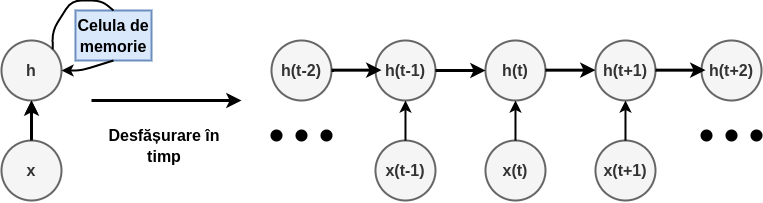
\includegraphics[scale=0.45]{unfolding}
					\caption{Derularea celulei recurente in timp. Figura apartine Goodfellow et al., 2016 \cite{dpb}.}
					\label{fig:unfolding}
				\end{figure}
				
				Celula de memorie este o denumire fictiva, ea referindu-se doar la mecanismul de prezervare a starii curente si transmiterii ei la celula recurenta dintr-un moment viitor. Acest lucru se realizeaza prin folosirea mai multor seturi de parametrii. Intr-o retea neuronala normala fiecare celula, neuron, este alcatuit dintr-un singur set de parametrii, ponderi, care se inmultesc matricial cu datele de intrare rezultand astfel gradul de activare al acelui neuron. Formula care sta la baza computatiilor din interiorul fiecarui neuron pentru o retea neuronala simpla  este $Y = W^T * X + b$, unde $Y$ este "activarea" neuronului iar $W$ si $b$  reprezinta parametrii antrenati. Daca un nivel dintr-o retea neuronala artificiala tradiionala contine mai multi neuroni, un nivel al unei retele recurente este alcatuita dintr-o singura celula distribuita pe mai multe puncte de timp. Spre deosibire de neuronul unei retele generice, celula RNN trebuie sa realizeze mai multe sarcini. Pe langa extragerea informatiilor din datele de intrade curente, de la momentul $t$, celula recurenta trebuie sa proceseze si starea de la momentul $t-1$ inanite de a determina iesire $y^{(t)}$ si starea curenta $h^{(t)}$. Din acest motiv pentru fiecare din aceste sarcini difeite se aloca un set de ponderii separat, de exemplu $U, W, V$ din Fig. \ref{fig:rnn_layer}.
				
				\begin{figure}[h]
					\centering
					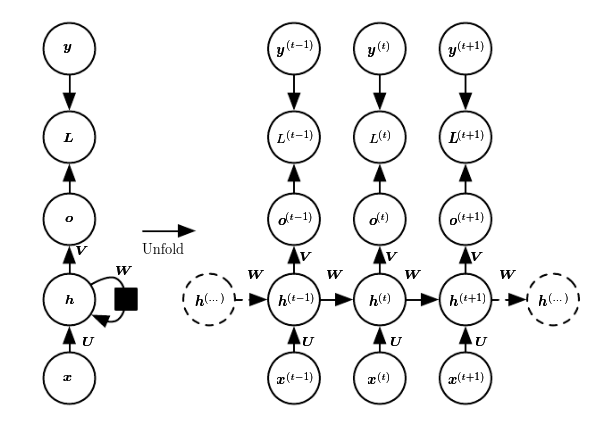
\includegraphics[scale=0.6]{rnn_layer}
					\caption{Desfasurarea procesului de antrenare pe intervalul de timp al datelor de intrare. La fiecare moement $t$ se calculeaza o eroare $L^{(t)}$ ca va genera modificarea tuturor ponderilor din $t$ si momentele predecesoare care au contribuit la aceasta. Figura apartine Goodfellow et al., 2016 \cite{dpb}.}
					\label{fig:rnn_layer}
				\end{figure} 
			Deoarece o celula recurenta foloseste un numar mai mare de parametrii, computatiile din interiorul acesteia devin mult mai complicate. Pentru o retea neruonala recurenta generica o celula poate fi descrisa prin urmatoarele ecuatii:
				
				\begin{align}
					a^{(t)} &= b + Wh^{(t-1)} + Ux^{(t)} \\ \label{rnn_states}
					h^{(t)} &= \tanh{(a^{(t)})}\\
					o^{(t)} &= c + Vh^{(t)}	
				\end{align}
				unde $a^{(t)}$ si $h^{(t)}$ reprezinta starea interna a celulei inainte si dupa aplicarea unei functii de activare, $o^{(t)}$ reprezinta valoarea la iesirea celulei, $U$ reprezinta ponderile datelor de intrare, $W$ reprezinta ponderile aferente starii precedente a retelei si $V$ ponderile de la iesirea celulei. \par
				
				Deoarece arhitectura unei celule recurente folosete seturi de parametrii diferite pentru cele doua intrari, stare precedenta si datele de intrare curente, aceasta poate controla atat impactul informatiilor acumulate din trecut cat si importanta datelor noi observate in prezent. Acesti parametrii, impreuna cu cei aferenti controlului iesirilor $V$,  sunt modificati in timpul antrenarii din doua perspective: reducerea erorii iesirii celulei de la timpul $t$, $L^{(t)}$,  si reducerea erorii adaugate de folosirea starii curente , $h^{(t)}$, in calculele iesiriilor celuleor de la momentele de timp viitoare, $L^{(t+1)}$, $L^{(t+2)}$, etc. \par
				
				Una din problemele depistate in cazul retelelor recurente este echilibrarea influentei introduse de starile de la momente de timp indepartate comparate cu cele de la momente de timp apropiate. Fiecare celula recurenta stabileste impactul stariilor precedente printr-o inmulitire matriciala cu un anumit set de parametrii, \ref{rnn_states}. Astfel, ponderea informatiilor unei stari dintr-un trecut indepartat poate scadea sau creste exponential. Daca neglijam functia de activare si "bias"-ul, pentru usurinta notatiei, sistemul de tranzitie a informatiilor recurente, starilor, in timp devine:
				\begin{align*}
				h^{(t)} &=  W^Th^{(t-1)} + U^Tx^{(t)}\\				
				h^{(t)} &=  W^T(W^Th^{(t-2)} + U^Tx^{(t-1)}) + U^Tx^{(t)}\\	
				h^{(t)} &= (W^2)^Th^{(t-2)} + W^TU^Tx^{(t-1)} + U^Tx^{(t)}\\	
				h^{(t)} &= (W^t)^Th^{(0)} + (W^{t-1})^TU^Tx^{(1)}+ ...+ W^TU^Tx^{(t-1)} + U^Tx^{(t)}
				\end{align*}
				Se poate astfel observa cum informatiile obtinute la starile anterioare sunt puternic influentate de distanta acestora fata de
				momentul prezent. Deoarece de obicei valorile ponderilor din $W$ sunt initializate cu valori mai mici decat 1, retelele neuronale recurente tind sa uite informatiile din starile incipiente dand o importanta mult mai mare celor din momentele de timp mai apropiate. In multe cazuri acest lucru nu este rezultatul dorit. Un exemplu ar fi crearea unui traducator dintr-o limba A intr-o limba B. Sensul unui cuvand aflat la capatul unei propozitsii poate depinde de unul din cuvintele de la inceputul propozitiei. Daca traducatorul uita de existenta acelui cuvand traducerea va fi in final una eronata.\par
				
				Pentru rezolvarea acestei probleme s-au propus noi arhitecturi ale celulelor care alcatuiesc retelele neuronale recurente. Una din aceste arhitecturi, si cea folosita de mine in acest proiect, este "Long Short-Term memory cell", sau LSTM. Diferenta dintr-o celula LSTM si una recurenta normala este folosirea unor asa numite porti care reusesc sa imbunatateasca capacitatea celulei de a controla informatiile pastrate sau uitate in procesul de antrenare recurenta.
				
				\begin{figure}[h]
					\centering
					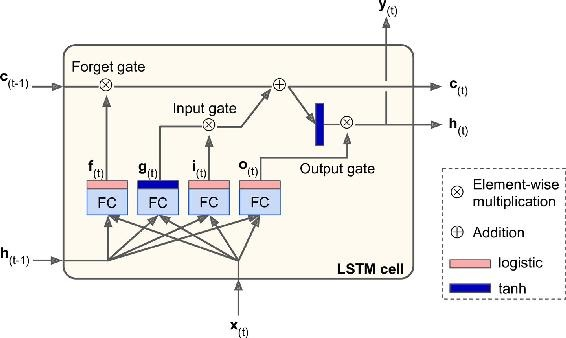
\includegraphics[scale=0.5]{lstm}
					\caption{Structura interna a unei celul recurente LSTM. Se pot observa conexiunile portilor care controleaza procesele din interiorul celulei: $f_{(t)}$, poarta de uitare, $g_{(t)}$ nivelul de procesare, $i{(t)}$ poarta de intrare si $o_{(t)}$ poarta de iesire. Figura apartine Gron, 2017 \cite{hands}}
					\label{fig:lstm}
				\end{figure} 
			
				Celulele LSTM folosesc doi vectori pentru memorarea starii celulei, unul pentru memorarea de lunga durata iar cel de al doilea pentru memorarea pe o durata scurta. In Fig.\ref{fig:lstm} putem obesrva arhitectura interna a unei astfel de celule si a portilor care determina transferul de informatie. \par
				 Fiecare din aceste porti sunt specializae in timpul antrenarii pentru rezolvarea anumitor sarcini specifice:
				\begin{enumerate}
					\item $g(t)$, reprezinta mecanismul principal de procesare de inforamtii din celula. Valorile obtinute la iesirea acestei parti din celula reprezinta valorile candidate care ar putea fi introduse in starea celuiei.  Intr-o celula normala, aceste valori ar trece direct in calcularea starii $h(t)$ si iesirii $y(t)$, fiind aferentul functiei $a(t)$ din \ref{rnn_states}. Intr-o celula LSTM insa, aceste valori sunt filtrate si abia apoi salvate in starea celulei prin folosirea portilor.
					\item $f(t)$, este denumita "forget gate", sau poarta de uitare, care controleaza care parti din memoria de lunga durata a celulei va fi uitata.
					\item $i(t)$, este denumita "input gate" sau "update gate", si decide ce valori din $g(t)$ ar trebui sa fie adaugate la memoria de lunga durata.
					\item $o(t)$, este denumita "output gate", si controleaza care parti din memoria de lunga durata ar trebui sa fie citite si folosite ca iesiri, atat pentru $h(t)$ cat si pentru $y(t)$. 
				\end{enumerate}
				Se poate observa cum in interiorul celulei LSTM se folosesc doua functii de activare diferite, functia sigmoid si tanh, prezentate in \ref{ml}. Functia sigmoid filtreaza cantitatea de informatie pe care fiecare poarta o cedeaza mai departe. Fiind urmata de o operatie de inmultire, daca o valoare din vectorul rezultat este 0 informatia aferenta acelei pozitii nu este transmisa in continuare. Cu cat acea valoare este mai apropiata de 1 cu atat informatia este transmisa mai complet. \par
				Transferul de informatie printr-o astfel de celula se face de la stanga la dreapta, Fig.\ref{fig:lstm}. In primul rand, poarta de uitare, $f(t)$, va filtra memoriile de lunga durata semnificative provenite din $c(t-1)$ luand in considerare memoria de scurta durata de la momentul anterior, $h(t-1)$, si datele de intrare curente, $x(t)$. Functia $g(t)$ produce noul set de informatii obtinute prin combinarea starii trecute cu datele de intrare. Aceste valori sunt apoi inmultite cu rezultatul portii de "update" care decide care din aceste informatii merita stocate in memoria "long-term", fiind adunate la aceasta. Dupa ce varianta reinointa a memoriei de lunga durata este obtinuta, $c(t)$, este conectata la o iesire a celulei si la o alta functie de activare tanh. Poarta de iesire, $o(t)$, transoformand aceste valori in iesire celulei, $y(t)$, cat si noua memorie de scurta-durata, $h(t)$. \par
				Astfel celula LSTM poate sa recunoasca care din datele de intrare sunt importante si sa le stocheze in starea de lunga durata, prin poarta de input, sa invete sa le pastreze pentru cat timp sunt relevante , prin poarta de uitare, si sa le extraga oricand le considera necesare, folosind poarta de iesire. Succesul obtinut de celulele LSTM in captarea relatiilor temporale de lunga durata poate fi explicat prin utlizarea acestor succesiuni de porti de control. Totusi, acest succes a fost demonstrat si intr-o maniera empirica prin folosirea unor baze de date special concepute pentru aceasta sarcina (Bengio et al., 1994; Hochreiterand Schmidhuber, 1997; Hochreiter et al., 2001) dar si prin aplicarea lor in diferite probleme din lumea inteligentei artificiale. \par
				
				Retelele neuronale recurente au avut mult succes in recunoasterea emotiei in vorbire. Motivul pentru care am ales sa folsoesc acest tip de retele a fost capacitatea acestora de a determina relatii temporale intre segmentele inregistrarilor audio. Deoarece emotia nu apare doar intr-un singur segment, fractiune de secunda, ci aceasta este prezenta pe intreaga durata a semnalului audio, obtinerea  conexiunilor temporale dintre informatiile emotiilor prezente in aceste segmente este cruciala. 
				
				\section{Mecanismul de atentie} \label{attention}
				 Mecanismului de atentie este bazat  pe principiul de functionare a perceptiei umane. Omenii  isi focuseaza atentia in mod selectiv, doar pe anumite parti din spatiul vizual sau auditoriu, pentru a extrage informatia necesara atunci cand este nevoie. Odata extarsa, aceasta informatie este combinata cu cea obtinuta din alte puncte de atentie pentru a crea o reprezentare interna a scenei \cite{zhang, attention1}. \par
				In SER, acest mecanism are ca scop identificare segmentelor inregistrarii audio cu o mare incarcatura emotionala si indreptarea atentiei modelului pe aceste segmente in timpul antrenarii. Din punct de vedere matematic, dorim sa obtinem un set de parametrii $\alpha_i$, unde $i$ ia valori intre 1 si numarul de segmente extrase, $L$, care sa functioneze ca ponderi reprezentative pentru importanta emotionala a fiecarui segment.
				\begin{equation}
					r = \sum_{i=1}^{L} \alpha_i s_i
				\end{equation}
				unde $\alpha_i$ reprezinta ponderea unui segment iar $s_i$ reprezinta datele aferente segmentului $i$. \par
				Mecanismul de atentie poate fi interpretat ca o medie ponderata a datelor din fiecare segment. Calcularea ponderilor folosite in aceasta medie se realizeaza prin adaugarea unui nou nivel de parametrii care vor fi antrenati sa depizeteze emotiile din fiecare segmente in forma uramtoare.
				\begin{equation} \label{softmax_form}
					\alpha_i = \frac{\exp(w^Th_i)}{\sum_{t=1}^{L} \exp(w^Th_t)}
				\end{equation}
				unde $w$ reprezinta ponderile antrenate.
				Aceasta functie se numeste "softmax" si are ca rezultat un vector egal cu numarul segmentelor extrase. Pentru fiecare segment se obtinute un numar intre (0,1), care poate fi interpretat ca probabilitatea ca acel segment sa fie bogat in informatie emotionala.  Parametrii $w$ sunt antrenati in timpul procesului de invatare impreuna cu restul modelului de clasificare.
		
		\chapter{Descrierea implementarii}
				Dupa cum am mentionat si in capitolele anterioare, proiectul meu este alcatuit din doua parti principale: modelul "Machine Learning" pentru recunoasterea emotiilor in semnale audio si interfata grafica pentru utilizator. Prima parte reprezinta solutia propusa pentru consturirea unui model SER iar cea de a doua face ca aceasta solutie sa poata fi antrenata, testata si utilizata intr-un mod accesibil, oferind o gama de functionalitati.\par 
				Diagrama din Fig. \ref{fig:uml}, ilustreaza distributia claselor folosite si relatiile dintre acestea. Se poate observa cum exista un numar mare de module de procesare de date, aferente diferitelor moduri de extragere a caractersiticitlor semnalului audio dar si a diferitelor functionalitati, ca antrenare si testare, inferenta si inferenta in timp real (online). Clasa care sustine interfata grafica (UI\_MainWindow) apeleaza aceste moduri de utilizare in functie de actiunile utilizatorului. \par
				
				Lucrarea de diploma a fost implementata in limbajul de programare Python, flolsind cadrul de programare specializat pentru dezvoltarea aplicatiilor Machine Learning, Tensorflow \cite{tensorflow}. Mai exact pentru a eficentiza inmultirile matriciale care stau la baza oricarei operatii din spatele modelelor ML, am folosit o versiune speciala numita \textit{tensorflow-gpu}, care realizeaza oricare astfel de operatie matematica folosind placa video. Aceste tipuri de procesare sunt specializate sa lucreze cu date din domeniul video, devenind mult mai eficiente cand vine vorba de inmultiri matriciale de dimensiuni mari. Avantajul obtinut prin folsoirea acestei versiuni de Tensorflow este marirea  vitezei de antrenare a modelelor. Pentru extragerea semnalului din fiserele audio, realizarea interfetei grafice si a functionalitatii de inregistrarea online am folosit diferite librarii specifice prezentate in urmatoarele subcapitole. \par
				\begin{figure}[p]
					\hspace*{-1,5cm}
					\centering
					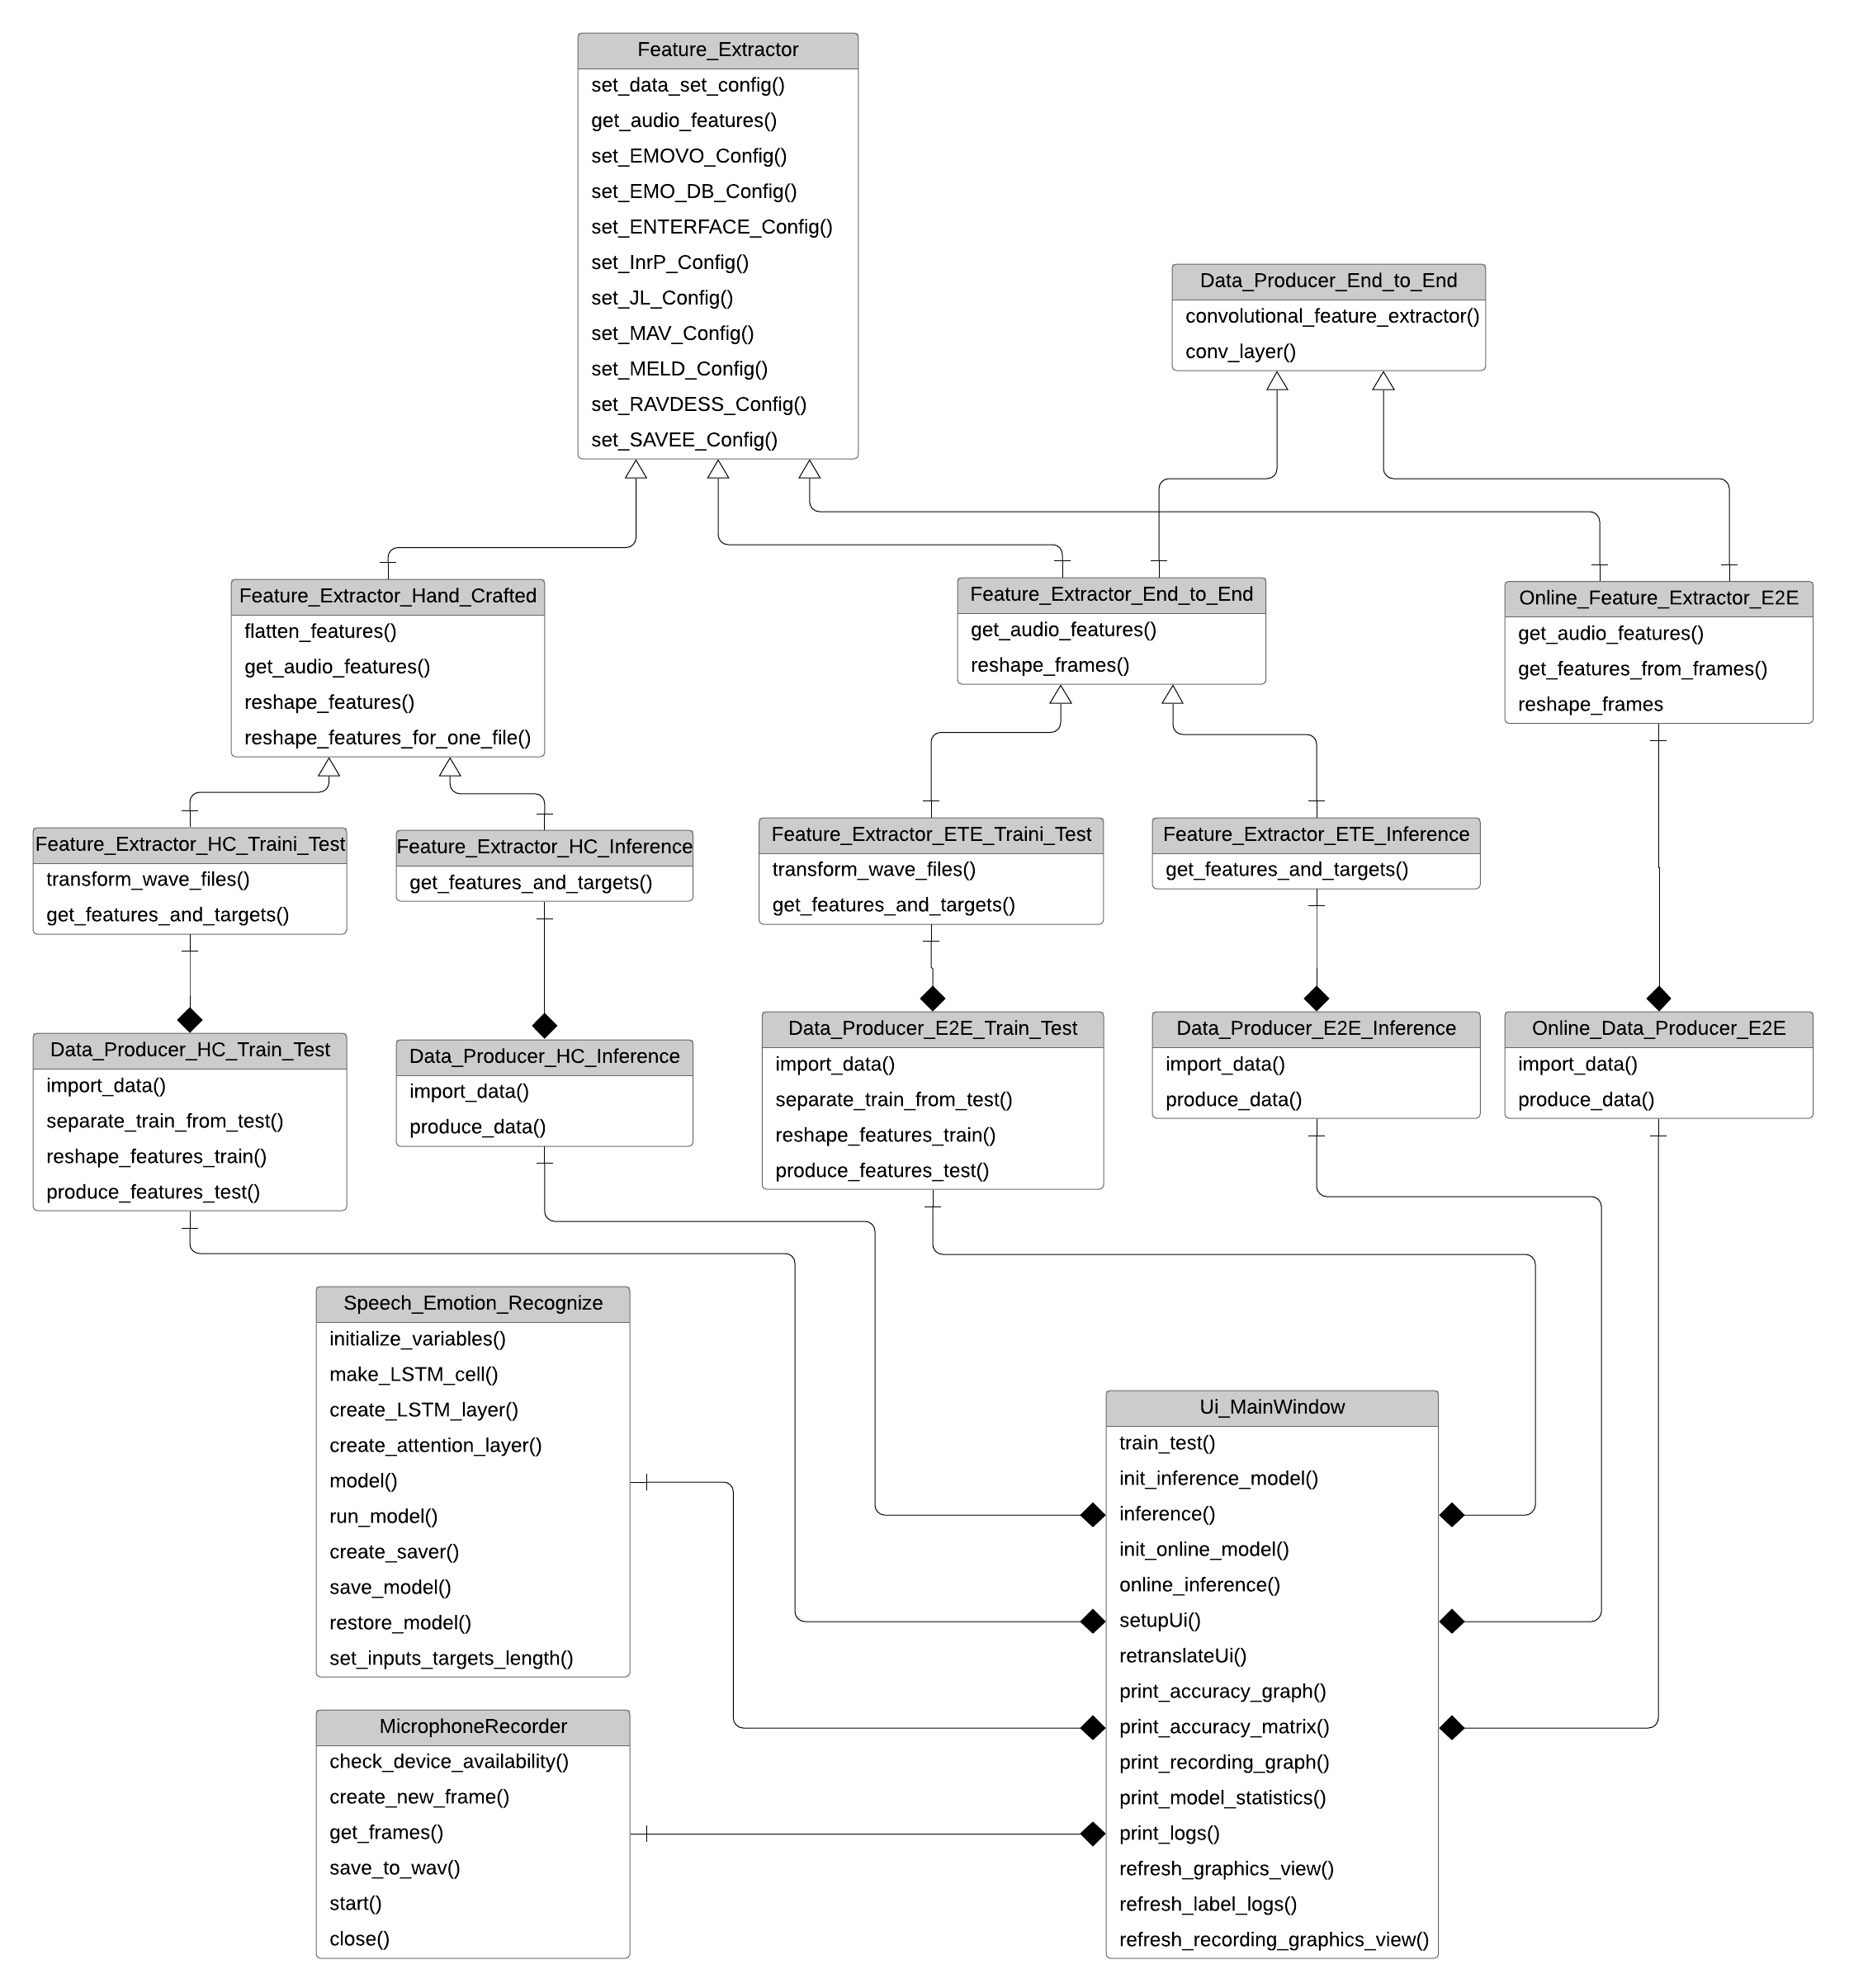
\includegraphics[scale=0.56]{uml}
					\caption{Diagrama UML ilustrativa a distributiei claselor proiectului. Utilizatorul are acces la intregul set de functionalitati al aplicatiei prin interfata grafica implementata in clasa \textit{UI\_MainWindow}.}
					\label{fig:uml}
				\end{figure} 
			
				\section{Modului de implementare a sistemului de recunoastere a emotiilor}
				
				Dupa cum am mentionat si in capitolul \ref{introdP}, un model "Machine Learning" de clasificare tipic trebuie sa realizeze trei sarcini: preprocesarea datelor, extragerea caracteristicilor de intrare si clasificarea propriu-zisa. Arhitectura propusa de mine pentru realizarea unei solutii pentru problema recunoasterii emotiei este ilustrata in Fig. \ref{fig:model}. In capitolul precedent am prezentat o descriere teoretica a algoritmilor folositi pentru construirea unui astfel de model, urmand ca in acest capitol sa prezint modul in care aceste concepte teoretice au fost implementate.
				
					\subsection {Bazele de date folosite} \label{datasets}
					In conextul domeniului SER una din principalele probleme este numarul redus de exemple din majoritatea bazelor de date existente. Cu toate ca in ultimii ani au aparut baze de date noi, care folosesc un numar mai mare de exemple, acestea nu sunt publice si necesita sume destul de mari de bani pentru accesul la date. Din aceste motive am decis sa folosesc mai multe baze de date publice in limbi si configuratii de inregistrare diferite. Pe langa aceste baze de date profesioniste, am decis sa adaug si un set de inregistrari proprii pentru a familiariza modelul cu configuratiile microfonului meu si pentru a contribui la majorarea numarului de exemple pentru antrenare.\par
					
					\newpage
					Bazele de date pe care le-am folosit sunt urmatoarele: EMO-DB, RAVDESS, SAVEE, EMOVO, MAV, ENTERFACE, JL si InrP.
					
					\begin{itemize}
						\item EMO-DB \cite{emodb} este o baza de date in limba germana, continand aproximativ 500 de inregistrari jucate de 10 actori in contextul a 6 emotii: fericire, enervare, anxietate, frica, plictisire, dezgust si neutru. 
						
						\item RAVDESS \cite{ravdess} contine 1440 de fisiere audio care reprezinta inregistrari jucate de 24 de actori profesionisti aferente a 7 emotii: neutru, fericire, tristete, enervare, frica, surpindere si dezgust. Limba in care au fost inregistrate aceste emotii jucate a fost engleza, cu un accent nord-american.
						
						\item SAVEE	
										
						\item EMOVO \cite{emovo} este o baza de date care contine 588 de inregistrari audio a 7 emotii dezgust, frica, enervare, fericire, surpiza, tristete si neutru. Inregistrarile au fost obtinute prin angajarea a 6 actori.
						
						\item MAV \cite{mav} sau "Montreal Affective Voices" este alcatuita din 90 de inregistrari nonverbale corespunzand unui set de 8 emotii: enervare, dezgust, frica, durere, tristete, surprindere, fericire ,placere si neutru, inregistrate de 10 actori.
						
						\item ENTERFACE \cite{enterface} contine 1320 de inregistrari audio, care surpind 6 emotii: enervare, dezgust, frica, fericire, tristete si surpindere in 14 limbi diferite.
						
						\item JL \cite{JL} este alcatuita din 2400 inregistrari din 240 de propozitii jucate de 4 actori in contextul a 5 emotii: enervare, tristete, neutru, fericire, entuziasm.
						
						\item InrP reprezitna setul de inregistrari personale.							
					\end{itemize}
				
				\subsection{Preprocesarea datelor}
					Tipul datelor de intrare folosite de modelul propus de mine sunt fisierele audio, mai exact fisierele cu extensia .wav care este cea mai folosita extensie pentru stocarea inregistrarilor audio in bazele de date SER existente. Incarcarea valorilor amplitudinilor semnalului audio intr-o matrice de stocare se realizeaza folosind o librarie specifica pentru porcesarea semnalului audio in Python, numita \textit{librosa} \cite{librosa}. Aceasta librarie ofera o gama larga de functii pentru procesarea semnalelor audio,  urmand sa fie prezentate in subcapitolul explicativ pentru extragerea caracteristicilor de intrare \ref{fex}.
					
					Pentru alcatuira setului de date am folosit inregistrari din diferitele baze de date prezentate mai sus. Inregistrarile fiecarei baze de date au fost realizate folosind diferite frecvente, variind intre 16KHz si 48KHz. Pentru a reduce memoria folosita cat si a  timpului necesar pentru antrenare (de la 12h la aproximativ 4h) am decis sa re-esantionez fisierele audio cu o frecventa de 16KHz folosind libraria librosa. Teorema lui Nyquist ne spune ca folosind o rata de esantionare de 16KHz putem surpinde fara pierderi orice semnal cu frecvente mai mici sau egale cu 8KHz. Aceast frecvente este mai mult decat necesara pentru captarea vocii umane care nu depaseste in contexte normale mai mult de 4KHz. Din punct de vedere empiric nu am gaist nici un dezavantaj in a folosit mecanismul de re-esantionare, sistemul SER obtinand aceasi acuratete in acelasi numar de epoci cu sau fara aceasta tehnica. \par
					
					Inainte ca semnalul audio sa poata fi folosit pentru extragerea informatiilor emotionale, acesta trece printr-un proces de partitionare in segmente de lungime fixa. Acest lucru ne permite sa aplicam transformatele fourier, sau alte functii asemanatoare, pe portiuni mai mici din semnalulu initial, obtinand o descriere mai detaliata a acestioa. Pentru a reduce datele pierdute intre segmente, de obicei se alege un pas de lungime mai mica decat dimensiunea segmentelor. Astfel o parte din informatia segmentului actual va fi prezenta si in cel viitor. \par 
					Urmatoarea etapa a procesului de preprocesare este aplicarea unor functii fereastara pe fiecare "frame". Acest lucru este realizat pentru a reduce pierderea de informatii la aplicarea transformarilor Fourier din cauza discontinuitatii de la marginea segmentelor. Functiile fereastra sunt functii care converg la zero in afara unui anumit interval. Inmultind un segment cu o astfel de functie are ca rezultat disparitia discontinuitatiilor de la marginea segmentului, similar cu privitul printr-o fereastra normala. Functia fereastra folosita se numeste "Hann-window", numita dupa Julius von Hann, si are formula urmatoare. \par
					\begin{equation}
					w[n]=\sin^2(\frac{\pi n}{N})
					\end{equation}.
					
				\subsection{Extragerea caracteristicilor de intrare} \label{fex}
				Semnalul audio nemodificat nu este cea mai eficienta modalitate de reprezentare a informatiei emotionale dintr-un discurs. Din acest motiv exista modalitati, functii matematice, care sa puna in lumina caracteristicile semnalului audio pentru a putea fi interpretat de sistemele SER in detectarea emotiilor. Aceste formule aplicate direct pe semnalul audio au fost prezentate in subcapitolul \ref{hand-crafted} pentru caracteristicile de intrare "hand-crafted" si \ref{end-to-end} pentru extragerea caracteristicilor antrenabila. \par
				
				In primul caz, extragerea caracteristilor de intrare ca coeficientii cepstrali mel (MFCC) sau delas si delta-deltas s-a relizeazat prin folosirea functiilor aferente prezente in libraria \textit{librosa}. Pentru ca extragerea acestor date sa fie corecta si pentru ca rezultatele obtinute sa aibe dimensionalitatea dorita a fost nevoie sa caluclez lungimea potrivita a segmentelor, marimea pasului de la un segment la altul, marimea functiei fereastra etc. \par
				
				\begin{lstlisting}[language=Python, caption={Extragerea caracteristicilor hand-crafted, 3.3, folosind libraria librosa.}, xleftmargin=0cm]
 def _get_audio_features(self, wav_file):
		signal, rate = librosa.load(wav_file,  self.hz)
		mfcc = librosa.feature.mfcc(y=signal, sr=rate, hop_length=260, 
									n_mfcc=20)
		delta = librosa.feature.delta(mfcc)
		delta_deltas = librosa.feature.delta(delta)
		rms = librosa.feature.rms(y=signal, frame_length=640, 
								hop_length=260)
		zcr = librosa.feature.zero_crossing_rate(y=signal, 
								frame_length=640, hop_length=260)
		chroma = librosa.feature.chroma_stft(y=signal, sr=rate, n_fft=820, 
								win_length=640,	hop_length=260)
		rolloff = librosa.feature.spectral_rolloff(y=signal, sr=rate, 
								n_fft=820, win_length=640, hop_length=260)
		features = [mfcc, delta, delta_deltas, rms, zcr, chroma, rolloff]
		return features	\end{lstlisting}
				
				In cel de al doilea caz am folosit libraria librosa doar pentru a aduce semnalul audio la o forma care eficientizeaza procesul de antrenare al retelelor neuronale convloutionale. Astfel am extras spectograma Mel, \ref{mel}, folosind functia corespunzatoare din libraria \textit{librosa}. Rezultatul obtinut este o imagine de dimensiuni 128x128 pentru fiecare din segmentele semnalului audio. Aceasta imagine este apoi normalizata si transmisa retelei convolutionale care se ocupa cu extragerea automata a informatiei emotionale. Deoarece reteaua convolutionala este la randul ei antrenata in timpul procesului de invatare, caracteristicile extrase de aceasta vor fi mai specifice sarcinii de recunoasterea a emotiei decat cele folosite in metoda "hand-crafted". \par
				
				\begin{lstlisting}[language=Python, caption={Extragerea spectogramei Mel, 3.4.1, folosind libraria librosa.}, xleftmargin=0cm]
  def _get_audio_features(self, wav_file):
		signal, _ = librosa.load(wav_file, self.hz)
		librosa.core.time_to_frames
		stft = librosa.feature.melspectrogram(signal, n_fft=512, 
							   win_length=128, hop_length=32, center=False)
		return stft	\end{lstlisting} \par
				Arhitectura reteli convolutionale folosite este prezentata in \ref{end-to-end}, iar secventa de cod care realizeaza aceasta functionalitate este ilustrata in Alg. \ref{cnn_code}. \par 
				Functia \_convolutional\_feature\_extractor exte responsabila pentru a crea modelului retelei convolutionale. Parametrul de intrare \textit{stft} reprezinta vectorul de spectograme Mel aferente segmentelor unei anumite inregistrari si este transmis primului nivel al retelei convolutionale. \par
				Fiecare nivel al retelei convolutionale este constiuit folosind metoda \textit{conv\_layer}. In aceasta metoda se creaza parametrii antrenabili din fiecare nivel, Alg.\ref{cnn_code} linia 5, in functie de dimensiunea filtrelor si a datelor de intrare. Parametrii obtinuti sunt transmisi functiei \textit{tf.nn.conv2d} a librariei Tensorflow care va crea nivelul convolutional specializat pe date in doua dimensiuni. \par
				Pentru primul nivel dimensiunea filtrelor a fost aleasa de \textit{8x8x1} pixeli iar numarul acestor filtrii este de 32, \textit{channels\_out}. Intre nivele retelei am folosit functia de activare $tanh$, urmata de functia de subesantionare maxim din libraria Tensorflow, \textit{tf.nn.max\_pool}. Motivatia folosirii acestor functii fiind descrise in sectiunile \ref{ml} respectiv \ref{cnns}.
				
				Tehnica numita "batch normalization", \ref{batch-norn}, este implementata prin normalizarea  valorilor rezultate in urma functiei  "max\_pooling" dupa fiecare nivel al acestei retele. \par 
				Cel de al doilea nivel este construit in aceasi modalitate ca si primul doar ca contine 16 filtre de dimensiunea \textit{4x4x32}. La final rezultatul care ajunge sa aibe dimensiunea \textit{(4 * nr\_segmente)x16x16} este aplatizat si adus la forma \textit{(4*nr\_segmente)x256} pentru a deservi ca intrare pentru reteaua neuronala recurenta. 
				\begin{lstlisting}[language=Python, caption={Implementarea nivelelor convolutionale care realizeaza extragerea caracteristicilor in maniera end-to-end folosind procedurile librariei Tensorflow.}, xleftmargin=-1cm, label=cnn_code]
class Data_Producer_End_to_End(object):
	def conv_layer(self, input_data, filter_size, channels_in, channels_out, 
						strides, conv_layer_dropout, name="Conv"):
		W = tf.get_variable("Weights_"+name+"_Layer", dtype=tf.float32, 
				shape=[filter_size, filter_size, channels_in, channels_out])
		return tf.nn.tanh(tf.nn.dropout(tf.nn.conv2d(input=input_data, 
													filter=W, 
													strides=strides, 
													padding='SAME', 
													use_cudnn_on_gpu=True), 
													conv_layer_dropout))
					
	def _convolutional_feature_extractor(self, stft, conv_layer_dropout):
			self.init = tf.glorot_normal_initializer()
			with tf.variable_scope("Convbb", reuse=tf.AUTO_REUSE, 
									initializer=self.init):
				stft = batch_normalization(stft)
				conv1 = self.conv_layer(input_data=tf.expand_dims(stft,axis=3),
										filter_size=8, 
										channels_in=1, 
										channels_out=32, 
										strides=[1, 2, 2, 1], 
										conv_layer_dropout=conv_layer_dropout, 
										name="conv1")			
				conv2 = tf.nn.max_pool(conv1, [1,2,2,1], [1,2,2,1], 
										padding="SAME")
				conv2 = batch_normalization(conv2)
				conv3 = self.conv_layer(input_data=conv2, 
										filter_size=4, 
										channels_in=32,
										channels_out=16, 
										strides=[1, 2, 2, 1], 										conv_layer_dropout=conv_layer_dropout, 
										name="conv2")				
				conv3 = tf.nn.max_pool(conv3, [1,2,2,1], [1,2,2,1], 
										padding="SAME")
				conv3 = batch_normalization(conv3)
				conv_out = tf.reshape(conv3, (-1, 256))
				return conv_out	\end{lstlisting}		
			
			\subsection{Clasificatorul sistemului SER} \label{clasif_prac}
				In Fig.\ref{fig:model} se poate observa cum modulul clasificator este alcatuit din doua celule bidirectionale recurente pe doua nivele urmat de mecanismul de atentie si de un nivel neuronal "dens". Fiecare din aceste componente aduce un anumit avantaj arhitectural care urmeaza sa fie prezenat in continuare. \par
				
				Retelele recurente, \ref{RNN}, spre deosebire de alte tipuri de retele neruonale reusesc sa determine nu doar informatiile emotionale de la un anumit moment de timp, ci si relatiile temporale intre emotii din diferite momente. Astfel emotii prezente in inceputul inregistrarii o sa aibe o anumita influenta si asupra emotiilor recunoscute la finalul acesteia. In construirea modulului neuronal recurent am decis sa folosesc doua celule LSTM bidirectionale, \ref{fig:lstm}, pentru a marii acuratetea sistemului SER. Termenul bidirectional inseamna ca o celula va procesa inregistrarea de la inceput spre final in timp ce cea de a doua va procesa aceasi informatie in sens invers, de la final spre inceput. In mod normal retelele recurente se folsoesc de informatia actuala si cea din trecut pentru a lua decizia la momentul curent, totusi exista aplicatii, ca si SER, unde decizia la momentul t poate fi influentata si de date prezenta la t+1. Un exemplu ar fi "speech recognition", unde intonatia unei litere poate depinde de litera care o urmaza, "co-articulatie", sau chiar de cuvintele urmatoare ( e.g. cuvantul "the" in limba engleza se pronunta diferit dace e urmat de un cuvant care incepe cu o vocala sau consoana). In recunoasterea de emotii in vorbire emotia fluctueaza intr-o conversatie. Oamenii pot intuii anumite expresii de astfel emotii, de exemplu cand cineva spune o gluma si bufneste in ras la final. Algorimtii de detectie a emotiilor ar trebui sa reuseasca si ei sa se foloseasca de informatii viitoare, "intuiri", pentru a determina emotia din prezent. \par
				Pentru a marii numarul gradelor de libertate ale retelei recurente, si in final maririi acuratetii modelului, am folosit pentru ambele tipuri de traversari ale semnalului audio doua nivele neuronale. Codul aferente acestui modul este prezentat mai jos.\par

				\begin{lstlisting}[language=Python, caption={Implementarea celulelor LSTM bidirectionale pe doua nivele folosind procedurile specifice ale librariei Tensorflow.}, xleftmargin=0cm]
def make_lstm_cell(self, hidden_size):
	cell = tf.contrib.rnn.LSTMCell(num_units=hidden_size, 
							use_peepholes=True, 		
							initializer=tf.glorot_uniform_initializer())
	if self._is_training and self._keep_prob < 1:
		cell = tf.contrib.rnn.DropoutWrapper(cell, 
										input_keep_prob=self._keep_prob,
										output_keep_prob=self._keep_prob, 
										variational_recurrent=True, 
										dtype=tf.float32, 
										input_size=hidden_size)
	return cell

def create_LSTM_layer(self, inputs, hid_size, name=None):
	with tf.variable_scope(name):
		lstm_cells_fw = [self.make_lstm_cell(hid_size) for _ in range(2)]
		lstm_cells_bw = [self.make_lstm_cell(hid_size) for _ in range(2)]
		multi_cell_fw = tf.contrib.rnn.MultiRNNCell(lstm_cells_fw, 
												state_is_tuple=True)
		multi_cell_bw = tf.contrib.rnn.MultiRNNCell(lstm_cells_bw, 
												state_is_tuple=True)
		initial_zero_state_fw = multi_cell_fw.zero_state(1, tf.float32)
		initial_zero_state_bw = multi_cell_bw.zero_state(1, tf.float32)
		inputs = tf.expand_dims(inputs, axis=0)
		outputs, _ = tf.nn.bidirectional_dynamic_rnn(multi_cell_fw, 
									multi_cell_bw, inputs, 
									initial_state_fw=initial_zero_state_fw, 
									initial_state_bw=initial_zero_state_bw)
		return tf.concat(outputs, 2)[0]				\end{lstlisting}
		Prima functie, \textit{make\_lstm\_cell} va crea celula recurenta LSTM, primind ca parametrii numarul de "neuroni" interni, care este egal pentru fiecare poarta, \textit{hidden\_size}. Daca modelul se afla in timpul procesului de antrenare se poate folosii tehnica de regularizare numita \textit{dropout}. Aceasta tehnica va dezactiva o anumita parte (1 - \textit{keep\_prob}) din reteaua recurenta in mod aleator pentru fiecare tranzitie prin retea. Prn acest mecanism se elimina dependentele puternice intre neuroni, care poate duce la procesul de "overfitting". Fenomenul de "overfitting" apare atunci cand modelul deivne mult prea bine specializat pe datele de antrenare si ajunge sa nu generalizeze bine pe datele de test, avand rezultate slabe in acest caz. \par
		Functia \textit{create\_LSTM\_layer} este cea care creaza intreg modulul recurent prin concatenarea celulelor recurente generate de  \textit{make\_lstm\_cell}. In listele \textit{lstm\_cells\_fw} si \textit{lstm\_cells\_bw} sunt stocate cele doua nivele recurente, celule LSTM,  care sunt date apoi ca parametru tunctiei din libraria Tensorflow \cite{tensorflow}, \textit{tf.nn.bidirectional\_dynamic\_rnn}. Aceasta functie va crea reteaua neuronala, oferind celulelor din \textit{lstm\_cells\_fw} datele de intrare in de la inceput spre sfarsit si celor din \textit{lstm\_cells\_bw} in sens invers. Rezultatele celor doua seturi de nivele recurente este salvat in \textit{outputs}. Varianta concatenata este retrunata de aceasta functie, reprezentand iesirile acestui modul. \par
		
		Rezultatele care reies in urma procesarii recurente a datelor sunt transmise mecanismului de atentie prezentat in \ref{attention}. Cum am spus si mai sus aceasta parte a sistemului SER are rolul de accentua informatiile din segmentele bogate in emotii si de a le neglija pe cele care pot sa aduca o nota de ambiguitate in procesul de clasificare. \par
		
		\begin{lstlisting}[language=Python, caption={Metoda care implementeaza mecanismul de atentie, \ref{attention}.}]	
def create_attention_layer(self, frame_predictions, weigths_dim):
	W = tf.get_variable("Attention_Weights", dtype=tf.float32, 
					shape=[weigths_dim, 1])
	b = tf.get_variable("Attention_Bias", dtype=tf.float32, shape=[1])	
	alpha = tf.matmul(frame_predictions, W) + b
	alpha = tf.nn.softmax(alpha, axis=0)
	return tf.expand_dims(tf.reduce_sum(tf.multiply(frame_predictions, 
						alpha[: tf.newaxis]), axis=0), axis=0)		\end{lstlisting}
		Functia care implementeaza tehinca de atentie este destul de scurta. In prmul rand, se creaza ponderile $W$ si "bias"-ul $b$ cu dimenisunea rezultatelor modulului recurent aferente fiecarui segment. Aceste ponderi sunt inmultite matricial cu datele fiecarui segment urmate de aplicarea functiei \textit{softmax} \ref{softmax_form} pe rezultate. In acest moment fiecarui segment i s-a atribuit un coeficient de "importanta" \textit{alpha}, ramanand doar ca acesti coeficenti sa fie inmultiti cu valorile rezultate in urma modulului recurent si sa se adune valorile obtinute pentru a realiza suma ponderata descrisa si la  \ref{attention}. \par
		
		Odata ce mecanismul de atentie a fost folosit informatiile din diferitele semgente ale semanlului audio au fost comasate intr-un singur set obtinandu-se astfel rezumatul informatiei emotionale a intregii inregistrari audio. Aceste set este transmis unui nivel neuronal simplu care are rolul de a reduce dimensiunea acestui rezumat emotional si de a oferi la iesire probabilitatea ca inregistrarea curenta sa apartina uneia din cele 4 emotii clasificate: enervare, fericire, tristete si neutru. \par
		
		Functia care leaga toate aceste componente si creaza modelul propus in arhitectura din \ref{fig:model} este urmatoarea.
		
		\begin{lstlisting}[language=Python, caption={Functia care creaza graficul de executie Tensorflow, conectand toate componentele de procesare ale sistemului SER.}]	
def model(self):
	with tf.variable_scope("Speech_Emotion_Recognizer", reuse=tf.AUTO_REUSE
						,initializer=self.init):
		rnn_layer = self.create_LSTM_layer(self._inputs, 
										self._hidden_size, 
										"Reccurent_Module")		
		attention_layer_output = self.create_attention_layer(rnn_layer, 
												self._hidden_size*2)
		predictions_1 = tf.layers.dense(attention_layer_output, 
										self._emotion_number, 
										name="Output_Layer")
		predictions = tf.reduce_sum(predictions_1, axis=0)		
		targets_raw_ = tf.nn.softmax(predictions, axis=0)		
		targets_ = tf.cast(tf.equal(targets_raw_, 
									tf.reduce_max(targets_raw_)), 
									tf.float32)
		if self._is_inference:
			self.predictions_raw = targets_
			self.predictions = targets_raw_
				return					
		self.label_pred = tf.argmax(targets_raw_)
		self.label_true = tf.argmax(self._targets)		
		self.accuracy = tf.cast(tf.equal(self.label_pred, self.label_true),
								tf.float32)
		if not self._is_training:
			return
		cross_entropy = tf.nn.softmax_cross_entropy_with_logits_v2(
													labels=self._targets, 
													logits=predictions)	
		adam_opt = tf.train.AdamOptimizer(self._learning_rate)
		self.optimizer = adam_opt.minimize(cross_entropy)	\end{lstlisting}
		Functia \textit{model} foloseste caracteristicile extrase de reteaua convolutionala in cazul end-to-end sau de formulele matematice predefinite in cazul hand-crafted prin parametru \textit{self.\_inputs}. Aceste caracteristici sunt transmise modulului recurent care este apoit conectat la mecanismul de atentie si la nivelul reteli neuronale dense numit "Output\_Layer". Rezultatele acestui nivel au dimensiunea \textit{self.\_emotion\_number}, in cazul nostru 4, pe care se aplica functia \textit{softmax} pentru a fi reprezntative din punct de vedere probabilistic. Pentru a fi aduse intr-un format de genul [0,0,1,0], rezultatele sunt comparate cu probabilitatea maxima, memorand 1 daca sunt egale si 0 in caz contrar. \par
		
		Daca modelul este folosit in cazul de inferenta dupa linia 17 se returneaza predicia obtinuta, care este afisata in interfata UI. \par
		In schimb, daca se executa procesul de testare este salvata emotia clasificata si cea adevarata pentru crearea statisticilor ilustrate in interfata UI si se determina daca predictia a avut succes (daca emotia clasificata este egala cu cea adevarata) la linia 23. \par
		In cazul in care modelul se afla in timpul antrenarii se calculeaza eroarea, sau mai exact functia de "loss", care ne spune exact cat de departe a fost modelul de a prezice corect emotia. Functia folosita de obicei in cazul clasificarii de mai multe clase mutual exclusive se numeste "cross entropy", $L = -\sum_{i=1}^{K} y_i \log(P_i)$ unde $K$ este numarul de clase, $y_i$ este valoare adevarata a clasei i (0 sau 1) iar $P_i$ este probabilitatea clasei $i$. Daca $y_i$ are valoarea 1, cea corecta, iar probabilitatea este apropiata de 1 atunci eroarea, L, are o valoare foarte mica. In schimb daca probabilitatea este mica prin aplicarea logaritmului negativ se va obtine o valoare mare. \par
		Aceasta valoare a erorii, alaturi de rata de antrenare, sunt oferite ca parametru de intrare unui optimizator care are rolul de a realiza mecanismul numit "backtracking", prin care se vor actualiza valorile ponderilor din interiorul reteleor neuronale, convolutionale, recurente, mecanismul de atentie si cea densa, pentru a reduce eroarea deteminata la pasul curent. Optimizatorul folosit este numit Adam \cite{adam} ("Adaptive momement estimation") deoarece este mult mai rapid decat tipurile de optimizatori traditionali ca, "gradiend descent". Acest optimizator fiind o extensie a algoritmului "gradient descent"	care foloseste diferite rate de invatare pentru parametrii interni si asa numite "momente" care sunt functii matematice care determina cand invatarea poate fi accelerata fara pierderea acuratetii. Eficienta acestui algoritm a fost demonstrata in varioase implementari, fiind unul dintre cei mai folositi optimizatori in domeniul "Machine Learning".
	\section{Implementarea si utilizarea interfetei grafice}
		Interfata cu utilizatorul ofera doua moduri de utilizare, pentru antrenare si pentru inferenta. Primul mod permite utilizatorului sa aleaga diferite configuratii de parametrii pentru antrenarea modelului si sa observe statistici in timp real asupra evolutiei acestuia. Cel de al doilea mod este orientat pe partea aplicativa a sistemului SER, permitand utilizatorului sa determine emotia predominanta din diferite fiesre audio pre-inregistrate sau chiar sa isi inregistreaz propriul discurs pentru inferenta. Cele doua moduri de utilizare vor fi descrise in subcapitolele urmatoare, impreuna cu cateva imagini care sa prezint exact interfata grafica. \par 
		Utilizatorul poate alege pe care din cele doua moduri doreste sa le foloseasca prin doua butoane radio \textit{Train} si \textit{Inference}. Butonul \textit{Start} incepe sa execute actiunea aleasa anterior. \par
		
		Pentru realizarea acestei interfete am folosit libraria PyQt5, care este o varianta a celebrei librarii pentru realizarea elementelor grafice din limbajul de programare C++. Tema folosita pentru aplicatie a fost realizata in libraria qdarkgraystyle, oferind culoarea si textura entitatiilor grafice din interfata, ca butoane, comboBox-uri etc. 
		
		\subsection{Interfata grafica in modul de antrenare} \label{guiAntrenare}
		
		\begin{figure}[h]			
			\centering
			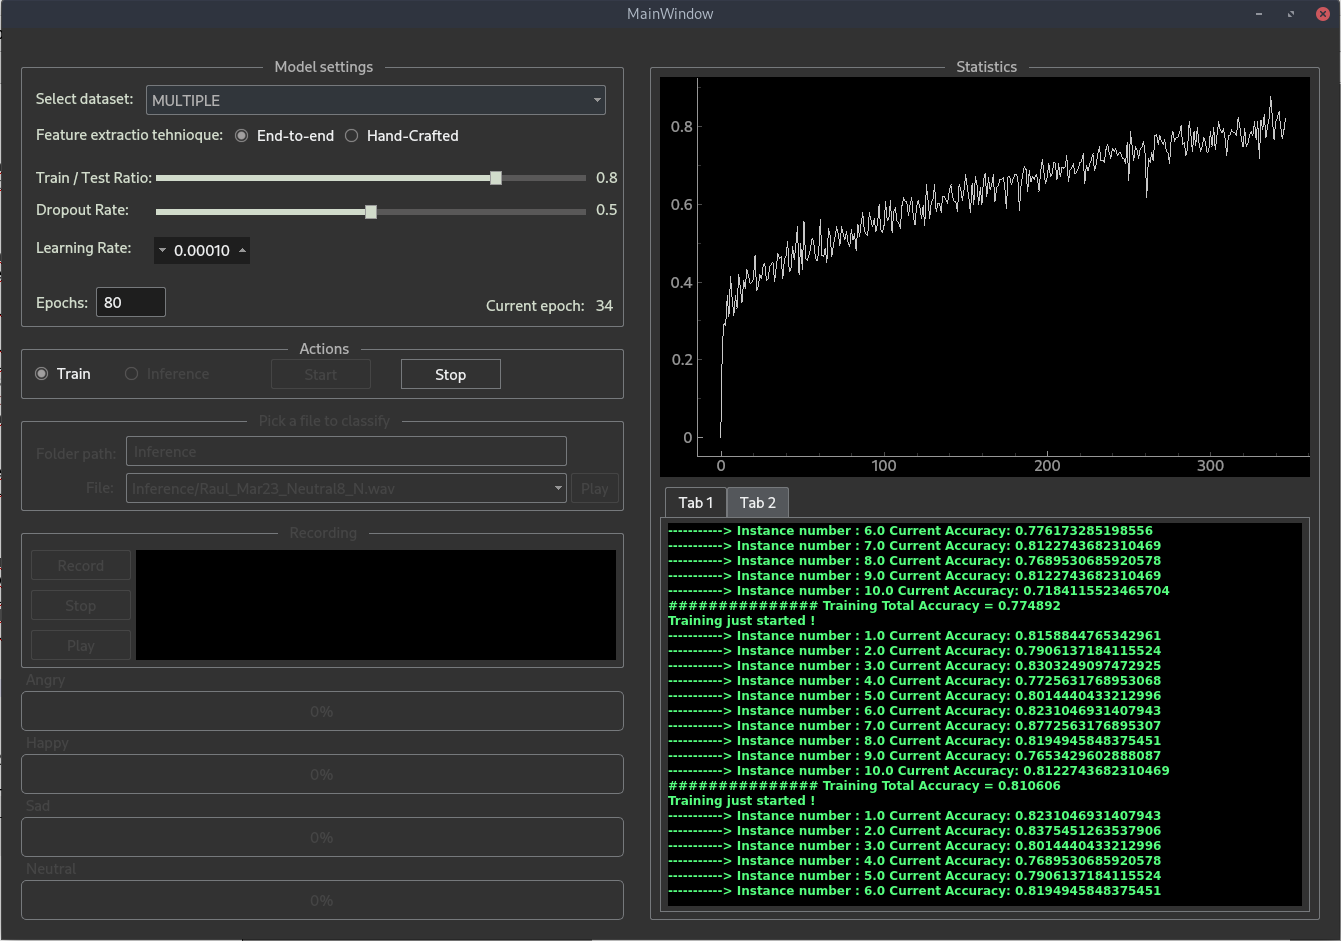
\includegraphics[scale=0.35]{gui_training}
			\caption{Interfata grafica in modul de antrenare}
			\label{fig:gui_train_1}
		\end{figure} 
		
		Interfata grafica in modul de antrenare, ilustrat in Fig. \ref{fig:gui_train_1}, ofera in partea stanga o serie de functionalitati de editare a parametriilor modelului in timp ce in partea dreapta se poate observa un grafic care prezinta evolutia modelului in timpul antrenarii si statisticile determinate in timppul procesului de invatare. \par
		In sectiunea "Model setttings" din interfata grafica utilizatorul poate sa controlzeze contextul in care se executa procesul de antrenare prin intermediul urmatorului set de parametrii:
		\begin{itemize}
			\setlength{\leftmargin}{-4cm}
			\item \textit{Select dataset}, este un comboBox care listeaza setul de baze de date care pot fi folosite pentru antrenare. Utilizatorul poate sa aleaga una dintre ele sau optiune Multiple, unde un numar din acestea au fost alese pentru a facilita optiunea folosirii unui numar mai mare de baze de date intr-o antrenare de tip "multi-domain".
			\item \textit{Feature extraction tehnique}, prezinta doua butoane tip radio prin care utilizatorul poate decide modul in care sunt extrase caracteristicile de intrare din semnalul audio.
			\item \textit{Train/Test Ratio} este un slider orizontal care permite utilizatorului sa decida ratia din setul de date utilizata pentru antrenare din baza de data aleasa la \textit{Select dataset}. Restul exemplelor vor fi folosite pentru testare.
			\item \textit{Dropout Rate}, este la fel un slider orizontal prin care utilizatorul decide probabilitatea ca un neuron sa fie activ in timpul antrenarii. Aceasta tehnica a fost prezentata si in \ref{clasif_prac}.
			\item \textit{Learning Rate}, este un text editabil prin care utilizatorul paote sa decida rata cu care se vor modifica ponderile in timpul antrenarii.
			\item \textit{Epochs}, este un text editabil in care utilizatorul mentioneaza numarul de epoci rulate in timpul antrenarii.
			\item \textit{Current epoch}, este un camp text needitabil care printeaza epoca in care se afla la acel moment procesul de invatare.			
		\end{itemize}
		Aplicatia seteaza o configuratie de parametrii recomandata la pornire dar utilizatorul poate sa faca diferite incercari modificand campurile sugerate mai sus. Dupa ce paramatrii au fost setati, prin apasarea butonului \textit{Start} se incepe antrenarea modelului. Deoarece am dorit sa prezint starea modelului in timp real pe parcursul invatarii, a fost nevoie sa creez un nou fir de executie pentru antrenare dupa apasarea butonului \textit{Start}. La anumite momente modelul va genera un set de informatii car vor fi transmise firului de executie principal pentru a le prezenta in zonele grafice aferente. Daca butonl care seteaza modul de executie este in starea \textit{Inference}, \textit{app.radioButton\_2}, apasarea butonului \textit{Start} va realiza clasificarea unuia din fiserele audio prezenta in directorul \textit{Inference}.
		
		\begin{lstlisting}[language=Python, caption={Metoda interfetei grafice apelata automat in urma apasarii butonului Start.}, label=on_click]	
def on_start_button_clicked(app):
	global thread_train
	if app.radioButton.isChecked():
		app.refresh_label_7()
		app.refresh_graphics_view()
		thread_train = Train_App(app)
		thread_train.print_accuracy_signal.connect(app.print_accuracy_graph)
		thread_train.print_stats.connect(app.print_stats_model)
		thread_train.print_matrix.connect(app.print_accuracy_matrix)
		thread_train.print_epoch.connect(app.print_label_19)
		thread_train.start()
	elif app.radioButton_2.isChecked():
		global ses, ser_inference_model, files
		vals = inference(ses, ser_inference_model, files ,
							app.comboBox_2.currentText()) * 100
	pass \end{lstlisting}
		\textit{Train\_App} reprezinta noul fir de executie cu ajutorul caruia se va antrena modelul. In secventa de cod de mai jos se poate obserca cum clasa \textit{Train\_App} mosteneste \textit{QtCore.QThread}. Odata instantiata aceasta clasa apeleaza functia \textit{run}, care contine apelul catre functia \textit{train}, care porneste procesul de invatare a modelului SER.
		\begin{lstlisting}[language=Python, caption={Clasa aferenta firului de executie pentru procesul de antrenare.}]	
class Train_App(QtCore.QThread):
	print_accuracy_signal = QtCore.pyqtSignal(float)
	print_stats = QtCore.pyqtSignal(str)
	print_matrix = QtCore.pyqtSignal(object)
	print_epoch = QtCore.pyqtSignal(str)
	stopFlag = False
	def __init__(self, app_rnning, parent=None):
		QtCore.QThread.__init__(self, parent)
		self.app_rnning = app_rnning
		
	def run(self):
		train(self, int(self.app_rnning.lineEdit.text()),
				float(self.app_rnning.horizontalSlider_2.value()) / 10,  
				float(self.app_rnning.horizontalSlider.value()) / 10, 
				float(self.app_rnning.doubleSpinBox.value()) ,
				map_config[self.app_rnning.comboBox.currentText()], 
				self.app_rnning.radioButton_3.isChecked()) \end{lstlisting}
		Functia train primeste parametrii care creaza contextul de executie al modelului, prezentati anterior, si incepe procesul de antrenare. In interiorul acestei functii se reseteaza graficul de executie \textit{Tensorflow} pentru procesul actual, se creaza noua sesiune \textit{Tensorflow}  pe care vom rula modelul, se creaza si apeleaza clasa care extrage caracteristicile de intrare din inregistrarile audio si incepe procesul de invatare. La finalul antrenarii este apelat modelul testor iar modelul antrenat este salvat pentru a putea fi folosit in modul de utilizare pentru inferenta. \par
		
		Statisticile sunt realizate in timp real prin intermediul informatiilor transmise din cadrul procesului de invatare. Libraria PyQt5 foloseste conceptul de semnale pentru actualizarea informatiilor din interfetele grafice. Astfel un semnal este emis din firul de executie pentru antrenare printr-o functie care este "conectata" la cea care modifica interfata grafica. Aceasta functie "conectoare" face parte din clasa firului de executie si modul de utilizare este ilustrat in 
		secventa de cod \ref{on_click}. \par
		Prima statistica ilustrata in interiorul apilcatieie este graficul care prezinta evolutia acuratetii modelului in timpul antrenarii. Acest grafic poate fi folosit pentru a determina anumite probleme care pot sa apara in timpul antrenarii sau pentru a determina cel mai favorabil numar de epoci. \par
		Cea de a doua statistica este una multipla, fiind alcatuita din doua pagini. Prima pagina are rolul de a instinta utilizatorul legat de procesele care i-au parte in interiorul modelului, de exemplu extragerea datelor dintr-un anumit set sau acuratetea atinsa pe datele de antrenare intr-o anumita epoca, si este ilustrata in Fig \ref{Fig:gui_train_logs}. Cea de a doua pagina, Fig \ref{Fig:gui_train_table}, reprezinta o matrice de confuzie care are pe coloane emotiile clasificate iar pe randuri emotiile adevarate. Astfel pe diagonala se vor afla numarul claselor identificate corect, iar in rest se va prezenta numarul de confuzii din fiecare caz.  
		\begin{figure}[h]
			\hspace{-1.2cm}
			\begin{minipage}{0.48\textwidth}
				\centering
				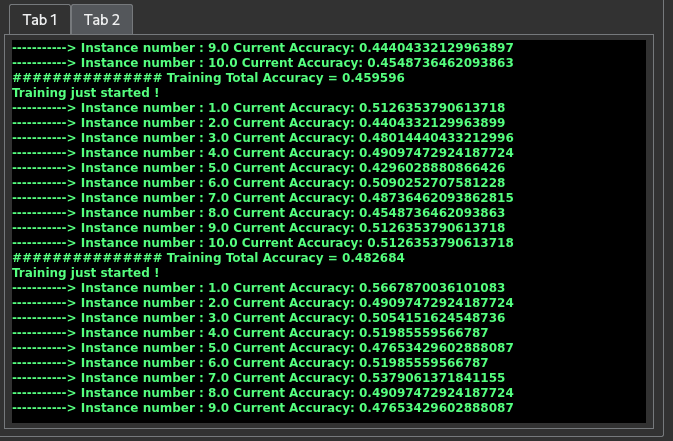
\includegraphics[scale=0.40]{gui_train_logs}
				\caption{Logarea progresului antrenarii.}\label{Fig:gui_train_logs}
			\end{minipage}\hfill
		\hspace{1.9cm}
			\begin{minipage}{0.60\textwidth}
				\centering
				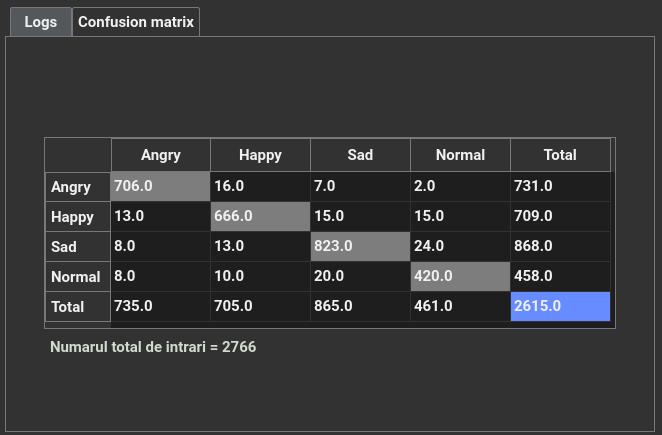
\includegraphics[scale=0.383]{gui_train_tabel}
				\caption{Matricea de confuzie a clasificatorului.}\label{Fig:gui_train_table}
			\end{minipage}
		\end{figure} 
		\subsection{Interfata grafica in modul de inferferenta}
		Modul de utilizare inferential este disponibil doar pentru extragerea datelor in varianta end-to-end. Din cauza limitarilor impuse de folosirea extragerii caracteristicilor in modul "hand-crafted", prezentate de-a lungul lucrarii, nu am putut garanta ca setul de caracteristici propus reuseste sa cuprinda in totalitate informatia emotionala. Astfel extragerea datelor in varianta "hand-crafted" este folosita doar pentru antrenare, ca un reper pentru varianta propusa, end-to-end. \par

		Interfata grafica este prezentata in Fig. \ref{fig:gui_inf}. Dupa cum se poate observa dupa apasarea butonului \textit{Inference}
		aplicatia dezactiveaza doate functionalitatile aferente modului de antrenare si le activeaza pe cele din modul inferenta. In acest mod utlizatorul are posibilitatea sa determine emotia din fisiere pre-inregistrate sau sa isi inregistreze pe loc propriile discursuri care vor fi clasificate automat dupa oprirea inregistrarii. \par
		
		In spatiul textului editabil \textit{Folder path} utilizatorul poate sa introduca calea pentru directorul in care se afla fisierele audio pre-inregistrate pe care doreste sa le clasifice. In mod implicit directorul folosit se numeste "Inference" si este inclus in directorul in care se afla proiectul. Combo box-ul \textit{File} enumera toate fisierele audio cu extensia .wav din acel director. Prin apasarea butonului \textit{Play} din dreapta acesteia utilizatorul poate auzi inregistrarea pe care doreste sa o clasifice. Pentru clasificare insa, este nevoie ca utilizatorul sa aleaga fisierul dorit si apoi sa apese pe butonul \textit{Start}. In urma acestui sir de comenzi probabilitatile aferente emotiilor clasificate vor fi ilustrate barele de progres \textit{Angry},  \textit{Happy}, \textit{Sad} si \textit{Neutral}. \par
		Recunoasterea emotiei in timp real este posibila prin apasarea butonului \textit{Record}. Odata apasat acest buton, aplicatia va incepe sa inregistreze prin microfonul implicit al calculatorului. Cand utilizatorul a terminat de inregistrat discursul pe care doreste sa il clasifice, pentru a determina emotia din acest discurs utilizatorul trebuie sa apese butonul \textit{Stop}. Butonul \textit{Stop} va opri firul de executie pentru inreigstrare, va salva discursul intr-un fisier audio si va oferi inregistrarea obtinuta modelului pentru clasificare. Ca si in cazul anterior, distributia de probabilitate a emotiilor va fi prezentata grafic in barele de progres aferente. \par
		\begin{figure}[h]
			\hspace{-0.7cm}
			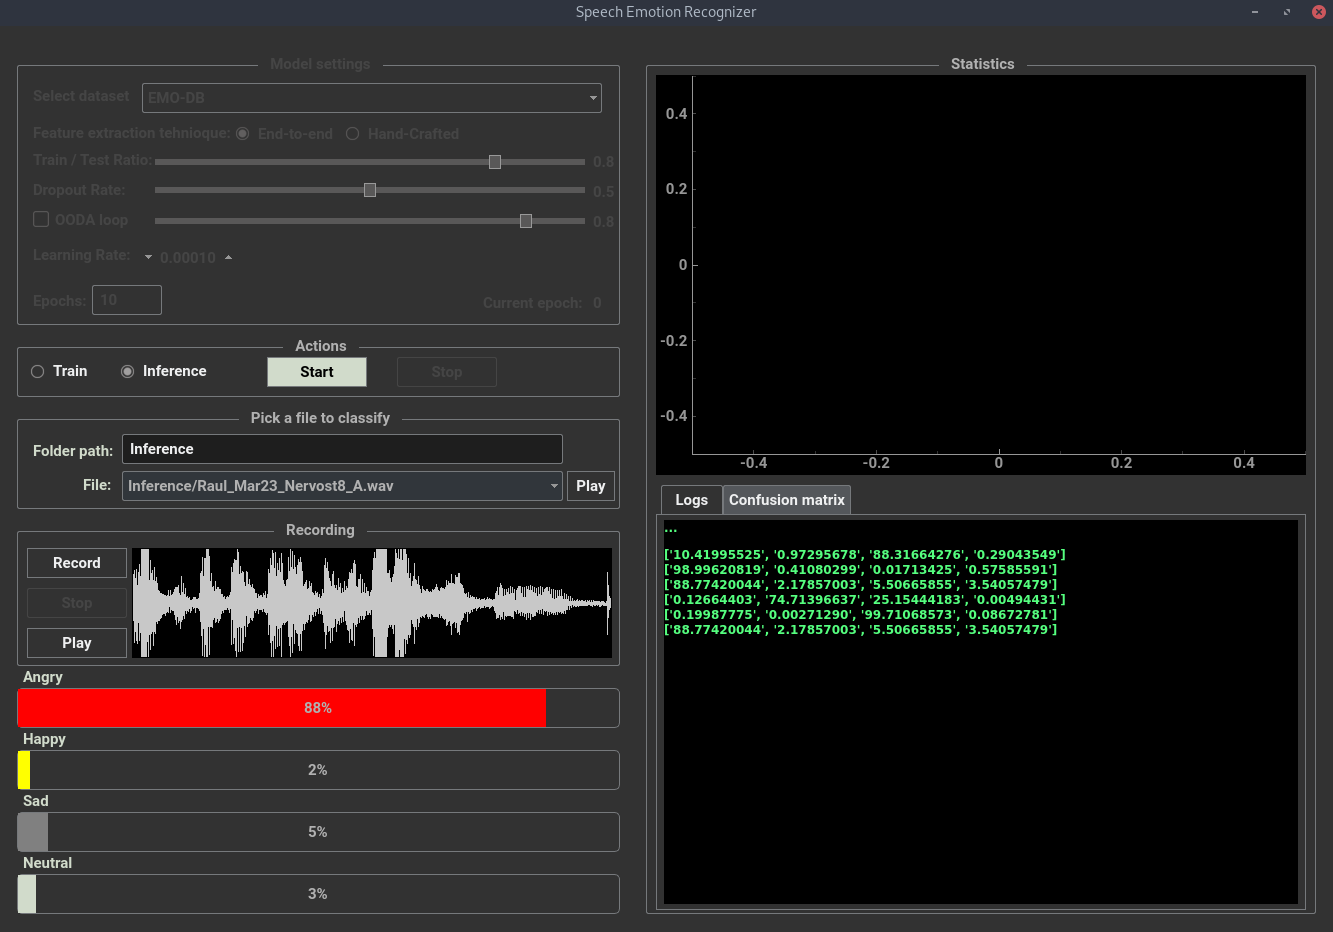
\includegraphics[scale=0.40]{gui_inf}
			\caption{Interfata grafica in modul de inferenta}
			\label{fig:gui_inf}
		\end{figure} 
		In timpul inregistrarii semnalul audio va fi proiectat in timp real in interfata grafica. Pentru a continua inregistrarea si a actualiza interfata grafica in acelasi timp, dupa apasarea butonului \textit{Record} se creaza un nou fir de executie special pentru procesul de inregistrare, asemanator cu crearea unui nou fir de executie pentru procesul de antrenare prezentat in sub-capitolul \ref{guiAntrenare}. Inregistrearea semnalului audio este realizata folosind libraria PyAudio iar proiectarea semnalului inregitrat este realizata prin memorarea unui set de amplitudini ale acestuia si proiectarea lor folosind libraria PyQt5 la o frecventa calculata in functie de rata de esantionare a semnalului. \par
		In timpul inregistrarii pot exista momente de liniste prelungite care daca persista pot influenta precizia clasificatorului. Pentru a reduce aceste momente la un minim s-a folosit libraria webrtcvad, care contine metode capabile sa determine existenta unui discrusi intr-un segment audio folosindu-se de anumite formule matematice asemanatoare cu cele prezentate in \ref{mel}. Secventa de cod care realizeaza inregistrarea si aceasta filtrare a vocii umane este ilustrat secventele de cod de mai jos.
		\begin{lstlisting}[language=Python, caption={Initializarea fluxului de transmitere a datelor pentru inregistrarea}]	
self.stream = pyaudio.PyAudio().open(format=self.sample_format,
									channels=self.channels,
									rate=self.rate,
									input=True,
									frames_per_buffer=self.chunk_size, 
									stream_callback=self.process_new_frame)

self.vad = webrtcvad.Vad()
self.vad.set_mode(1) \end{lstlisting}
		Functia \textit{open} a librariei PyAudio porneste un flux de date provenite de la microfon, care dupa ce atinge un numar de segmente egal cu valoarea \textit{self.chunk\_size} il transmite metodei \textit{self.process\_new\_frame}. Deoarece aceste linii de cod realizeaza functia de inregistrare valoarea parametrului \textit{input} este setata pe adevarat. Pentru a face functia opusa, ascultarea unui fisier audio, fluxul de date este creat aproximativ in aceasi metoda, modificandu-se valoarea parametrului input pe fals si setarea valoii parametrului output pe adevarat. \par
		
		In campul \textit{self.vad} se stocheaza o instanta a mecanismului de detectare a vocii si se seteaza drasticitatea filturlui pe valoarea 1, unde intervalul de agresivitate al acestuia este [0, 3]. \par

\begin{lstlisting}[language=Python, caption={Procesarea unui nou segmente al semnalului audio inregistrat. Daca segmentul nu contine discurs uman este exclus din inregistrarea finala.}]		
def process_new_frame(self, data, frame_count, time_info, status):
	data = np.frombuffer(data, dtype=np.int16)
	with self.lock:
		if self.vad.is_speech(data, self.rate):
			self.frames.append(data)
		if self._print_frames_count == self._print_chunk_size:
			self.thread.print_recording_signal.emit(self._print_frames)
			self._print_frames = np.array([])
			self._print_frames_count = 0
		else:
			self._print_frames = np.concatenate((self._print_frames,data), axis=0)
			self._print_frames_count+=1
		if self.stop:
			return None, pyaudio.paComplete
return None, pyaudio.paContinue	\end{lstlisting}
		Metoda \textit{process\_new\_frame} primeste in parametrul \textit{data} un set de segmente audio de lungime \textit{frame\_count}. Aceste segmente sunt verificate de mecanismult de detectie prin metoda \textit{self.vad.is\_speech} si in caz pozitiv sunt adaugate la setul de segmente care urmeaza sa fie clasificate de sistemul SER. \par
		Semnalul audio inregistrat este proiectat in interfata grafica prin folosirea metodei \textit{emit} a semnalului firului de executie de inregistrare \textit{self.thread.print\_recording\_signal}. In vectorul \textit{self.\_print\_frames} sunt salvate toate segmentele primite pentru a afisa intregul semnal in interfata audio. \par
		La apasarea butonului Stop din interfata grafica campul \textit{self.stop} va opri procesul de inregistrate generand salvarea semnalului intr-un fisier audio de tip .wav si pornirea clasificatorului.
		
		 
%---------------------------------------------------------------------------------------------------------------------------------------------		
		\chapter{Rezultate si experimente}
		 
		 In acest capitol vor fi prezentate rezultatele obtinute in urma executarii unui set de experminente prin care solutia propusa este testata in diferite configuratii. Rezultatele obtinute sunt apoi comparate cu cele ale altor arhitecturi din domeniu. Desi sistemul SER a fost implementat special pentru lucrul cu mai multe baze de date intr-o maniera "end-to-end", rezultatele obtinute atat in cazurile in care s-a folosit o singura baza de date cat si in cele in care extragerea datelor a fost de tip "hand-crafted" se mentin la nivelul celorlalte solutii SER.\par
			
		 Solutia propusa in aceasta lucrare de diploma este antrenata intr-o maniera "multi-domain", pe inregistrari care provin din baze de date diferite. Antrenarea "multi-domain" prezinta o serie de avantaje enumerate la \ref{datasets}, dar face ca compararea arhitecturii cu alte sisteme SER sa fie dificila. Din acest motiv, in continuare vor fi enumerate rezultatele obtinute de model in particular pentru unele din bazele de date care alcatuiesc setul descris la \ref{datasets}. \par
		 Antrenand modelul pe intreaga baza de date EMO-DB \cite{emodb}, cu inregistrari aferente a 7 emotii, acuratetea maxima inregistrata a fost de 77\%, in timp ce acuratetea medie a fost de aproximativ 75\%. Aceste rezultate sunt comparative cu cele obtinute de Kerkeni et al., 2018 \cite{comp1}, unde folosind un modul clasificator similar, doua celule recurente LSTM urmate de doua nivele dense, s-a obtinut o acuratete maxima de 73\% si una medie de 69.55\%. Una din cele mai de succes solutii SER antrenate pe aceasta baza de date este prezentata in Issa et al, 2020 \cite{comp2}, unde numarul inregistrarilor a fost marit prin folosirea unor tehnici de augmentare ca adaugarea unui nou set de exemple obtinut prin accelerarea la 1.23\% a inregistrarilor, incetinrea la 0.81\%, mutarea punctului de start, sau adaugarea unui zgomot la 25\% din lungimea inregistrarii. In urma acestei serii de augmentari, acuratetea modelului propus in Issa et al, 2020 \cite{comp2} a atins precizia de 82.86\%.\par
		 Baza de date RAVDESS \cite{ravdess} contine 1440 de inregistrari incorporand 8 emotii. Folosind inregistrari doar din acesata baze date pentru antrenare, modelul propus a obtinut o acuratete maxima de 71.08\% si una medie de 68\%. Acest rezultat este comparativ cu precizia inregistrata in Issa et al, 2020 \cite{comp2} de 71.61\%. Zeng et al., 2017 \cite{comp3} au obtinut o acuratete de 65.97\% folosind retele neuronale produnde si o antrenare tip "multi-task", antrenand modelul sa clasifice emotii atat in vorbire cat si in cantece. Folosind un model clasficator bazat pe retele neuronale convolutionale Popova et al., 2018 \cite{comp4} au inregistrat o acuratete de 71\% pe aceasta baze de date. \par
		 Realizand antrenarea calsificatorului pe 7 emotii folosind inregistrari din baza de date EMOVO \cite{emovo} s-a atins o acuratete maxima de 70\%. Rezultate similare au fost obtinute si in Latif et al., 2018 \cite{comp5}, acuratete de 76.22\%, unde clasificatorul sistemului SER a fost bazat pe o tipologie speciala de retele neuronale numite "Deep Belief Neural Networks". Latif et al., 2018 \cite{comp5} propun si folosirea tehnicii "transfer learning", prezentata la \ref{tehnici}, unde inaintea antrenarii pe baza de date EMOVO modelul este antrenat mai intai pe baze de date din alte limbi. Aceasta tehnica ii permite modelului sa depaseasca valoarea initiala a acuratetii atingand precizia de 80\%. \par 
		 Antrenand solutia propusa in aceasta lucrare pe baza de date ENTERFACE'05 \cite{enterface}, care contine inregistrari reprezentative pentru un set de 6 emotii, acuratetea maxima obtinuta a fost 83.26\%. Rezultate similare au fost obtinute in Schuller, 2011 \cite{comp6}, unde prin folosirea uni clasifiator traditional pentru probmela recunoasterii emotiei, "Support Vector Machine", s-a atins o precizie de 62.8\% pe aceasta baza de date. Rezultate mai promitatoare au fost obtinute in Ooi et al., 2014 \cite{comp7}, in care modelul propus inregistreaza precizia 75.89\%. \par
		 
		 Dupa cum se poate observa, chiar daca solutia propusa este de tip "multi-domain", rezultatele obtinute de sistemul SER implementat in aceasta lucrare se apropie considerabil de cele obtinute de implementari care sunt specializate pe cate una din acestea. Prin reducerea numarului de exemple pentru a cuprinde doar setul de emotii enumerat la \ref{solutie} (fericire, tristete, enervare si neutru), acuratetea pe fiecare din bazele de date depaseste rezultatele prezentate mai sus. In cazul bazei de date EMO-DB acuratetea maxima obtinuta pe cele 4 este de 91.04\%, in cazul RAVDESS 76.11\%, EMOVO 80.59\% si ENTERFACE'05 90.05\%.  
		 
		 \par		 
		 Un alt experiment a fost realizat prin modificare modului de extragere a caracteristicilor de intrare. Metoda "end-to-end", \ref{end-to-end}, este cea propusa pentru arhitectura finala a sistemului SER implementat in aceasta lucrare, totusi pentru a evidentia importanta acestei tehnici in continuare vor fi prezentate rezultatele inregistrate pentru clasificare bazata pe caracteristici "hand-crafted". Acuratetea maxima inregistrata in cadrul acestui experiment a fost de 68.56\%, iar acuratetea medie a fost de 67\%.
		 	
		 \par
		 Solutia propusa cuprinde atat o antrenare tip "multi-domain" cat si o extragere a caracteristicilor de intrare "end-to-end". Rezultatele obtinute folosind aceasta configuratie finala sunt incurajatoare fiind asemanatoare cu cele obtinute de o alta arhitectura SER antrenata intr-o modalitate asemanatoare. Acuratetea ne-ponderata maxima obtinuta de modelul propus in aceasta lucrare a fost de 84.1\%, avand o valoare medie de aproximativ 82\%. Aceste rezultate le depasesc cu aproximativ 15\% pe cele obtinute folosind caracteristicile "hand-crafted", subliniind beneficiile extragerii "end-to-end". In acelasi timp, desi era de asteptat ca acuratetea modelului sa scada folosind mai multe baze de date, se poate observa cum aceasta se mentine, si chiar depaseste, unele din preciziile inregistrare folosind cate una din bazele de date. Sistemul SER prezentat in Milner et al., 2019 \cite{multi-domain} profita de generalitatea obtinuta prin antrenarea "multi-domain" intr-o arhitectura SER similara cu cea implementata in aceasta lucrare, \ref{prez_multi_domain}. Acurateta ne-ponderata obtinuta in acest studiu a fost de 82.26\% pe 6 emotii diferite, fiind apropiata de cea obtinuta de mine chiar daca setul de baze de date si numarul de emotii clasificate difera. \par		 
		 
		 Din punct de vedere arhitectural solutia propusa poate fi comparata cu alte cateva din domeniul SER. Folosind o singura baza de date, dar acelasi mod de extragere a caracteristicilor de intrare, solutia prezentata in Li, Yuanchao et al., 2019 \cite{yuan}, a atins o precizie de 82.8\%, fiind una dintre cele mai inalte masurate pe baza de date IEMOCAP \cite{iemocap}. Misramadi et al., 2017 \cite{misramadi}, au introdus un modul clasificator bazat pe retele neuronale recurente bidirectionale combinate cu un mecanism de atentie, similar cu cel din acest proiect, si au obtinut o acuratete cu 3.1\% mai mare decate cea inregistrata pana in acel moment pe baza de date folosita de acestia. Alte rezultate cu arhitecturi apropiate de cea propusa de mine au fost:  Kerkeni et al. (2018) \cite{compar1} unde s-a inregistrat o acuratete de 82.14\% pe baza de date EMO-DB \cite{emodb}, Fonnegra et al., 2018 \cite{compar2} au obtinut rezultate promitatoare folosind baza de date ENTERFACE'05 \cite{enterface} cu o acuratete 92\%, Lim et al., 2016 \cite{compar3} au executat mai multe experminete pe baza de date EMO-DB \cite{emodb} obtinand precizii de 87.74\% intr-o arhitectura cu retele convolutionale, 79.87\% intr-o arhitectura cu retele neuronale recurente si 88.01\% combinand cele doua tipologii de retele neuronale intr-o maniera asemanatoare cu arhitectura folosita in aceasta lucrare de diploma. \par
%---------------------------------------------------------------------------------------------------------------------------------------------		 
		\chapter{Concluzii}		
		Lucrarea de diploma contine atat o solutie pentru recunoasterea emotiei in vorbire cat si o interfata grafica care permite antrenarea, testarea si inferenta eficienta a sistemului SER. Domeniul recunoasterii emotiei in vorbire nu este pana in acest moment unul "cucerit", prezentand o gama larga de obstacole care nu au permis obtinerea unei acurateti destul de satisfacatoare pentru a permite acestor algoritmi sa fie introdusi pe piata. Solutia implementata de mine reuseste sa atinga o acuratete comparabila cu a unor arhitecturi de success din domeniu si chiar sa le depaseasca in anumite configuratii. Aceasta acuratete este pusa apoi in practica prin interfata grafica care permite utilizatorului sa clasifice emotiile din interiorul discursurilor provenite din mai multe surse. \par		
		
		Sistemul SER propus incearca sa determine o arhitectura eficenta pentru rezolvarea recunoasterii de emotii in vorbire intergrand diferite tehnici si concepte cu scopul de a cuprinde cat mai complet complexitatea problemei. Alegerea folosirii unui set de mai multe baze de date este justificata de imbunatatirea generalitatii modelului "Machine Learning". Extragerea datelor in maniera "end-to-end" este motivata de lipsa unui set de caracteristici audio de intrare specializat pe recunoasterea emotiilor in vorbire. Implementarea unui modul clasificator bazat pe retele neuronale recurente este aleasa pentru a profita de relatiile temporale intre emotiile din segmente audio aflate la momente diferite. Urmarea retelei recurente de un mecanism de atentie este bazata pe filtrarea segmentelor lipsite de emotie pentru a reduce inconsistentele introduse de acestea. \par
				
		In construirea acestui proiect am folosit multe din tehnici invatate in decursul facultatii de Automatica si Calculatoare ca programarea orientata pe obiecte, dezvoltarea interfetelor grafice, programarea concurenta si diferite concepte ale inteligentei artificiale. Totusi, pentru realizarea unui sistem SER am necesitat informatii specifice care au fost obtinute prin studiul unor arthicole stintifice din domeniu, enumerate si in decursul lucrarii. Tehnologiile folosite au crescut in numar cu multimea de functinalitati adaugate incluzand limbajul de programare Python, celebra libraria Tensorflow pentru dezvoltarea aplicatiilor "Machine Learning", Librosa pentru extragerea informatiilor auditive, webrtcvad pentru identificarea semgentelor care contin voce umana si pyaudio pentru inregistrarea si redarea fisierelor audio. \par
		
		Scopul final al unui sistem SER este acela de a fi introdus in interfetele de comunicare om-masina din viitor, pentru a oferii masinilor capacitatea de a intelege conversatiile la care iau parte si dintr-un context emotional. Integrarea acestor algoritmi va creste calitatea conversatiilor permitand ca interfetele de comunicare om-masina sa atinga o calitate asemanatoare cu cele de la om la om. Pana a ajunge in acel punct insa, algoritmii de recunoastere a emotiilor trebuie sa mai treaca printr-o serie de imbunatariri pentru a creste gradual acuratetea inregistrata. Solutia propusa de mine reprezinta o arhitectura intr-o stare incipienta, avand potentialul de a fi extinsa prin introducerea mai multor tehnici. \par
		Prima modalitate de imbunatatire a sistemului SER propus, si cea mai simpla, ar fi marirea numarului de baze de date folosite pentru a amplifica si mai mult generalitatea modelului, sa combata problema numarului redus de exemple si sa mareasca numarul de emotii clasificate. \par 
		O alta modificare ar putea fi constituita din introducerea unui modul care sa diminueze diferentele dintre inregistrarile provenite din baze de date diferite. Algoritmi care realizeaza aceasta sarcina au fost deja introdusi in alte solutii din domeniu. De exemplu Deng et al. , 2014 \cite{imbun1} au folosit cu succes o tehnica numita "adaptive denoising-autoencoders", care invata sa determine si sa elimine diferentele dintre mai multe baze de date prin aducerea inregistrarilor acestora la o forma asemanatoare cu cele dintr-o anumita baza de data tinta. Alte tehinici de reducere a discrepantelor bazelor de date sunt normalizarea per baza de date sau normalizare per vorbitor, Bjorn et al, 2010 \cite{spnorm}. \par
		Tehinca antrenarii pe mai multe sarcini, "multi-task", poate la randul ei sa aduca imbunatariri puternice modelului clasificator. Prin antrenarea modelului pe o serie de sarcini in acelasi timp sistemul poate sa devina inflexibil la variatii ale semnalului audio care nu ar trebui sa influenteze emotia clasificata. Li, Yuanchao et al., 2019 \cite{yuan} au antrenat arhitectura SER popusa atat pe recunoasterea emotiilor in vorbire cat si pe determinarea sexului vorbitorului, in timp ce Milner et al., 2019 \cite{multi-domain} au folosita ca sarcina secundara determinarea bazei de date din care face parte inregistrarea curenta. Aceste doua tehnici s-au dovedit a fi avantajoase in combatarea influentei sexului vorbitorului cat si a bazei de date de provenienta in decursul procesului de clasificare.\par 
		O alta extindere a proiectului curent ar putea fi combinarea solutiei propuse cu un algoritm de detectie a emotiei vizuale. Astfel produsul final va putea determina emotia umana folosindu-se de doua tipuri diferite de stimului. Aceasta metoda s-a demonstratat a fi avantajoasa in difeite articole ca Tzirakis et al., 2014 \cite{tzir} sau Sana et al., 2010 \cite{imbun3}, unde s-a depasit acuratetea sistemului SER initiala prin adaugarea informatiei vizuale in clasificarea emotiilor. \par
		
		
		Proiectul meu de diploma prezinta astfel o solutie incipienta pentru una din problemele care au ramas inca nerezolvate in domeniul inteligentei artificiale, recunoasterea emotiei in vorbire. Lucrarea de diploma include atat un model "Machine Learning" clasificator cat si o interfata grafica care permite utilizatorului sa incerce diferite configuratii de parametrii, sa observe statistici detaliate ale proceselor care i-au parte in timpul antrenarii si sa incerce modelul antrenat pe inregistrari din diferite surse. Chiar daca sistemul SER prezentat nu este momentan viabil pentru a fi introdus pe piata rezultatele obtinute sunt asemanatoare cu cele prezente in unele dintre implementariile profesioniste de succes din domeniul recunoasterii de emotii in vorbire din prezent. Rezultatele incurajatoare sustin astfel ca solutia "Machine Learning" propusa are un potential puternic de a fi extinsa pentru a imbunatatii precizia curenta prin aplciarea unei game largi de tehnici existente sau a unora noi, care tind sa apara anual in acest domeniu. 
		
		
		\renewcommand{\clearpage}{}
		\addcontentsline{toc}{chapter}{Bibliografie}
		\printbibliography[title={Bibliografie},notcategory=cited,resetnumbers=true]
		%\hfil \\
		%\hfil \\
		\addcontentsline{toc}{chapter}{Referinte}
		\printbibliography[title={Referinte},category=cited,resetnumbers=true]
		\newpage
\end{document}




























